\documentclass{scrartcl}
\usepackage[utf8]{inputenc}
\usepackage{physics}
\usepackage{graphicx}
\author{Jakob S. Kottmann }
\usepackage{booktabs}
\usepackage{algorithmic}
\usepackage{algorithm}
\usepackage{amsmath}
\usepackage{amsfonts}
\usepackage{amssymb}
\usepackage{xcolor}
\usepackage{xspace}
\usepackage[sort&compress,numbers,super]{natbib}
\usepackage{doi}
\bibliographystyle{apsrev4-1}
\bibliographystyle{numeric}
\usepackage{tikz}
\usetikzlibrary{quantikz}

% colored boxes
\usepackage{amsthm}
\theoremstyle{definition}
\newtheorem*{algo*}{Algorithm}
\newtheorem*{theorem*}{Property}
\newtheorem*{ex*}{Example}
\newtheorem*{def*}{Def}

\definecolor{unia}{HTML}{3C2673}
\definecolor{fai}{HTML}{009b5d}
\definecolor{fai2}{HTML}{66c39e}
\definecolor{fai3}{HTML}{b3e1ce}
\definecolor{unia2}{HTML}{8c358b}
\definecolor{unia3}{HTML}{dbbfdd}
\definecolor{unia4}{HTML}{eddeee}

\usepackage{sectsty}
\allsectionsfont{\color{unia}\selectfont}
\renewcommand{\contentsname}{}

\usepackage[
breakable,
]{tcolorbox}
\tcolorboxenvironment{theorem*}{
colframe=unia,
colback=blue!10!white,
breakable,before skip=10pt,after skip=10pt}
\tcolorboxenvironment{ex*}{
colframe=yellow!50!black,
colback=yellow!10!white,
breakable,before skip=10pt,after skip=10pt}
\tcolorboxenvironment{algo*}{
colframe=unia,
colback=blue!10!white,
breakable,before skip=10pt,after skip=10pt}
\tcolorboxenvironment{def*}{
colframe=fai,
colback=fai3,
breakable,before skip=10pt,after skip=10pt}

\def\highlight{}
\def\endhighlight{}
\tcolorboxenvironment{highlight}{
colframe=yellow!50!black,
colback=yellow!10!white,
breakable,before skip=10pt,after skip=10pt}

% for explicit examples
\newcommand{\0}[0]{\ensuremath \mathbf{0}}
\newcommand{\1}[0]{\ensuremath \mathbf{1}}
\newcommand{\2}[0]{\ensuremath \mathbf{2}}
\newcommand{\3}[0]{\ensuremath \mathbf{3}}
\newcommand{\4}[0]{\ensuremath \mathbf{4}}
\newcommand{\5}[0]{\ensuremath \mathbf{5}}
\newcommand{\6}[0]{\ensuremath \mathbf{6}}
\newcommand{\7}[0]{\ensuremath \mathbf{7}}
\newcommand{\8}[0]{\ensuremath \mathbf{8}}
\newcommand{\9}[0]{\ensuremath \mathbf{9}}
\newcommand{\kk}[0]{\ensuremath \mathbf{k}}
\newcommand{\m}[0]{\ensuremath \mathbf{m}}
\newcommand{\n}[0]{\ensuremath \mathbf{n}}

\newcommand{\hd}[0]{\ensuremath\operatorname{H}}

% colored boxes end

\usepackage{listings}

\definecolor{brightred}{rgb}{1.00,0.00,0.00}
\definecolor{mediumgray}{rgb}{0.70,0.70,0.70}
\definecolor{olivegreen}{rgb}{0.49,0.56,0.16}
\definecolor{purple}{rgb}{0.68,0.00,0.49}
\definecolor{darkgreen}{rgb}{0.00,0.50,0.00}
\definecolor{steelblue}{rgb}{0.25,0.44,0.63}
\definecolor{darkteal}{rgb}{0.00,0.40,0.38}
\definecolor{brown}{rgb}{0.56,0.13,0.00}
\definecolor{brickred}{rgb}{0.73,0.13,0.13}
\definecolor{orange}{rgb}{0.74,0.48,0.00}
\definecolor{slateblue}{rgb}{0.02,0.16,0.49}
\definecolor{midblue}{rgb}{0.08,0.33,0.51}

\lstset{
  language=python,
  keywordstyle=\color{darkteal},
  commentstyle=\color{mediumgray},
  stringstyle=\color{brickred},
  identifierstyle=\color{midblue},
  numberstyle=\tiny\color{mediumgray},
  rulecolor=\color{mediumgray},
  backgroundcolor=\color{white},
  emphstyle=\color{brightred},
  basicstyle=\ttfamily\small,
  breaklines=true,
  numbers=left,
  numbersep=8pt,
  tabsize=2,
  showstringspaces=false,
  emph={int,float,str,list,dict,set,tuple,bool},
  emphstyle=\color{olivegreen},
  emph={[2]print,len,range,open,enumerate,zip,map,filter,sorted,sum,min,max,any,all},
  emphstyle={[2]\color{purple}},
  literate=
    {+}{{{\color{steelblue}+}}}1
    {-}{{{\color{steelblue}-}}}1
    {*}{{{\color{steelblue}*}}}1
    {/}{{{\color{steelblue}/}}}1
    {=}{{{\color{steelblue}=}}}1
    {==}{{{\color{steelblue}==}}}2
    {!=}{{{\color{steelblue}!=}}}2
    {<=}{{{\color{steelblue}<=}}}2
    {>=}{{{\color{steelblue}>=}}}2
    {@}{{{\color{steelblue}@}}}1,
  literate=*%
    {0}{{{\color{darkgreen}0}}}1
    {1}{{{\color{darkgreen}1}}}1
    {2}{{{\color{darkgreen}2}}}1
    {3}{{{\color{darkgreen}3}}}1
    {4}{{{\color{darkgreen}4}}}1
    {5}{{{\color{darkgreen}5}}}1
    {6}{{{\color{darkgreen}6}}}1
    {7}{{{\color{darkgreen}7}}}1
    {8}{{{\color{darkgreen}8}}}1
    {9}{{{\color{darkgreen}9}}}1
}

\usepackage{hyperref} 
\hypersetup{
    colorlinks,
    linkcolor={unia},
    citecolor={fai},
    urlcolor={fai}
}

\newcommand{\mathsc}[1]{\text{\normalfont\scshape #1}} % Proves small caps in math mode

\setlength{\parindent}{0cm}
\setlength{\parskip}{1em}

\usepackage{fancyhdr}
\pagestyle{fancy}
\lhead{Lecture notes SS26}
\rhead{JSK, Augsburg University}
\setcounter{section}{0}
\usepackage{comment}
\usepackage{schemata}
\excludecomment{forme}

\begin{document}
    
\thispagestyle{empty}
\begin{tikzpicture}[remember picture,overlay]
   \node[anchor=north east,inner sep=20pt] at (current page.north east)
              {
\includegraphics[height=3cm]{logo-fai.png}};
\end{tikzpicture}

\begin{tikzpicture}[remember picture,overlay]
   \node[anchor=north west,inner sep=10pt, align=left] at (current page.north west)
              {
\includegraphics[height=3cm]{UniA_Logo_RGB_InstInformatik_DE.png}};
\end{tikzpicture}

\begin{tikzpicture}[remember picture,overlay]
   \node[anchor=north,inner sep=120pt, align=center] at (current page.north)
              {
                \Large
                \textbf{Quantum Algorithms (SS 26)}\\
                \phantom{x}\\
                \large J.S. Kottmann\\
                \normalsize with contributions from A. Bärligea \& O. Hüttenhofer
                
              };
\end{tikzpicture}
\vspace{2cm}
\hrule

\tableofcontents
\clearpage
\section{Motivation and first Examples}
Quantum mechanics is the physical theory that describes elementary processes on the microscopic level. In this chapter we will touch the essential aspects of the theory from a quantum algorithmic perspective. At the end we will construct a small, but famous, quantum algorithm -- the \texttt{Deutsch} algorithm. Although it isn't very useful in practice, it is an excellent example that illustrates many important aspects of quantum mechanics in general, and quantum algorithmics especially.\\

Imagine an experiment with an elementary particle (e.g. an Electron or a Photon) which we can observe in two states labeled as $\ket{0}$ and $\ket{1}$. This could be the magnetic moment (``spin'') of the electron or the polarization of the photon. In the first case, you can imagine the observation of the spins allignment to be performed by switching on an external magnetic field, the field will then either increase or decrease a tiny bit (depending if the magnetic moment of the electron points in the same direction of the external or opposite). You can also imagine something more illustrative, like a coin that can be either heads or tails, or a marble in a double half-pipe or ``double-well''
\begin{align*}
    \ket{0}\equiv\raisebox{-0.9cm}{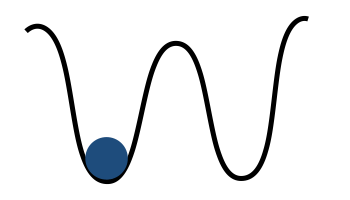
\includegraphics[width=0.25\textwidth]{src/doublewell-left.png}},\quad
    \lvert 1 \rangle \equiv \raisebox{-0.9cm}{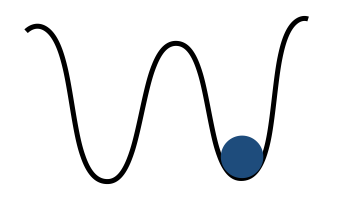
\includegraphics[width=0.25\textwidth]{src/doublewell-right.png}}
\end{align*}
that has two localized states: ``left'' and ``right'', which we just call the state $\lvert 0\rangle$ and $\lvert 1\rangle$.
For all examples given, we can just label the two states as 0 and 1 -- the $\ket{}$ notation is used to denote that $\ket{a}$ is the state that we labelled with the symbol $a$ (it is just more convenient than subscripts).\\
Classical realization of such binary systems are called \textit{bits}, while we call the quantum versions \textit{qubits}. A qubit, an idealized quantum two-state system, is therefore the quantum version of a bit, an idealized classical two-state system. \\

Now consider a ``coin-flip'' process $U$ that \textit{acts} on the \textit{state} of our particle.  If we observe the particle afterwards we can either find it in state $\ket{0}$ with probabilty $p_0 = \frac{1}{2}$ and in state $\ket{1}$ with probability $p_1 = \frac{1}{2}$ -- for both possible input states.\\

For the examples with elementary particles, you can imagine it like a black-box which the particle ``flies'' through and some physical interactions happen inside the box.
For our ``double-well'' example above, this process is basically placing the marble at the center where it will eventually fall down the right or left side (with a sufficient symmetric double-well potential, the probabilities will be fifty-fifty)

\begin{align*}
    \raisebox{-0.9cm}{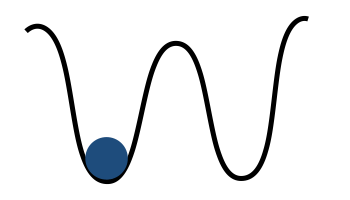
\includegraphics[width=0.25\textwidth]{src/doublewell-left.png}} \leftarrow \raisebox{-0.9cm}{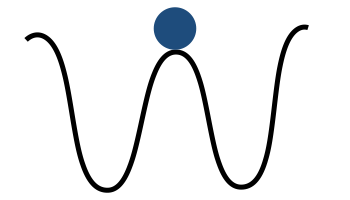
\includegraphics[width=0.25\textwidth]{src/doublewell-center.png}} \rightarrow \raisebox{-0.9cm}{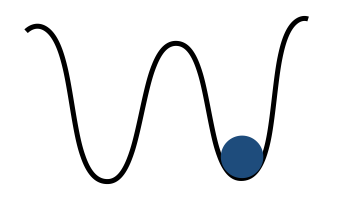
\includegraphics[width=0.25\textwidth]{src/doublewell-right.png}}.
\end{align*}
However, we are not aiming to find an exact mechanical description (how to realize the process for an explicit physical system), but rather a general description about the outcome of the process (ignoring the mechanical realization).


\subsection*{A Classical Probabilistic Process (Coin Flips)}
Let's describe the process $U$ as a classical process. To emphasize it, we will label it as $U_\text{C}$.
An obvious candidate that comes to mind is the description of $U_\text{C}$ as a probabilistic process that ``flips'' the particle with 50\% probability. The process takes the state $\ket{k}$ with $k \in [0,1]$ as an input and outputs $\ket{k\oplus 1}$\footnote{$\oplus$ denotes logical addition $k\oplus l = \left(k+l\right)\mod2$. Explicitly: $0\oplus0=0, 0\oplus1=1\oplus0=1, 1\oplus1=0$. The function $f(x) = x \oplus 1$ on bit value $x$ is for example the same as a logical \textsc{not} operation.} with 50\% probability. We could write it as
\begin{align}
    \ket{i} \xrightarrow{U_\text{C}}  \begin{cases} \ket{i} \text{ with } p=1/2 \\ \ket{i\oplus 1} \text{ with } \tilde{p}=1-p \end{cases}.
\end{align}
Now suppose a new process $U_\text{C}^2$ that executes the original process $U_\text{C}$ twice
\begin{align}
    \ket{k} \xrightarrow{U_\text{C}}  \xrightarrow{U_\text{C}} \ket{l}.
\end{align}

The end result $\ket{l}$ will either be $l=0$ or $l=1$ with probabilities of 50\%. We can see this by looking at the probabilities of all individual outcomes of the $U^2_\text{C}$ process
\begin{align}
      \ket{i} \xrightarrow{U_\text{C}} \begin{cases} \ket{i}\phantom{\oplus 0}
      \xrightarrow{U_\text{C}}
      \begin{cases} \ket{i}\phantom{\oplus 0}  \\ \ket{i \oplus 1} \end{cases} \\ \ket{i \oplus 1} \xrightarrow{U_\text{C}} \begin{cases} \ket{i\oplus 1} \\ \ket{i \oplus 1 \oplus 1} =\ket{i} \end{cases}  \end{cases}.  
\end{align}
The probabilitiy for each individual outcome is the product of the probabilities of the two individual processes $0.5\cdot 0.5 = 0.25$ and as $1\oplus 1 = 0$ we have only two different outputs of $U^2_\text{C}$, the two bit values $\ket{0}$ and $\ket{1}$ each with accumulated probability $0.5$. Our description of the given process as a probabilistic bit-flip with $p=0.5$ in series is therefore \textit{idempotent} which means $U_\text{C}^2 = U_\text{C}$.

\subsection{Quantum Process}

Another way that seems more complicated on first glance, is to allow \textit{superpositions}~\footnote{basically another word for \textit{linear combination}} of the states $\ket{0}$ and $\ket{1}$
\begin{align}
    \ket{\psi} = c_0\ket{0} + c_1\ket{1},\quad c_0,c_1\in \mathbb{C},
\end{align}
with the interpretation that the probability to observe the particle in $\ket{i}$ is given by $p_i = |c_i|^2$ for $i\in\left\{0,1\right\}$. We call the coefficients $c_i$ the \textit{probability amplitutes} for the \textit{basis state} $\ket{i}$. 
To ensure consistency with this probability interpretation, we need to enforce a normalization condition on the amplitudes
\begin{align}
    |c_0 |^2 + | c_1 |^2 = 1. 
\end{align}
The action of our process, in the quantum version denoted as $\hd$, is assumed to act \textit{linear} on such a superposition
\begin{align}
    \hd\ket{\psi} = c_0 \hd\ket{0} + c_1 \hd\ket{1}.
\end{align}

In order to describe our process, we can now define the action of $\hd$ on the two basis states as
\begin{align}
    \hd\ket{0} &= \frac{1}{\sqrt{2}}\left( \ket{0} + \ket{1} \right) \equiv \ket{+}, \\
    \hd\ket{1} &= \frac{1}{\sqrt{2}}\left( \ket{0} - \ket{1} \right) \equiv \ket{-}.\label{eq:U|1>}
\end{align}
At this point one might ask why the minus sign and the $\frac{1}{\sqrt{2}}$ factor enter the equations. Both have to do with the interpretability of the coefficients in the linear combinations as probability amplitudes. We have abbreviated the positive and negative superposition of the two basis states as $\ket{\pm}$, as we will encounter them again in later chapters. \\

At this point, the observable outcome of the process $\hd$ on the states $\ket{0}$ and $\ket{1}$ is the same as before: 50\% observed in the unchanged input state $\ket{k}$, and 50\% observed in the flipped state $\ket{k\oplus 1}$. 
If we however investigate the outcomes of $U^2$ the results change with respect to our classical description
\begin{align}
    \hd^2\ket{k} &= \frac{1}{\sqrt{2}} \hd \left( \ket{0} + (-1)^k \ket{1} \right),\\
    &= \frac{1}{2} \left( \ket{0} + \ket{1} + (-1)^k \ket{0} - (-1)^k \ket{1} \right),\\
    &= \frac{1}{2} \left( (1+(-1)^k)\ket{0} + (1 + (-1)^{k+1})\ket{1} \right)\label{eq:U2|k>}
\end{align}
or, with explicit values for the two choices of the input state $\ket{k}$:
\begin{align}
    \hd^2\ket{k} = \begin{cases}
        \ket{0} \text{ if } k=0 \\
        \ket{1} \text{ if } k=1
    \end{cases}
\end{align}
so that we can write
\begin{align}
    \hd^2\ket{k} = \ket{k}
\end{align}
meaning we will always observe the unchanged input state after the process $\hd^2$ -- the process $\hd$ is \textit{self-inverse} (or \textit{involutory)}. This differs from our classical process $U_\text{C}^2$! The reason for this is the negative probability amplitude introduced in Eq.~\eqref{eq:U|1>} that leads to \textit{destructive interference} of the amplitudes in Eq.~\eqref{eq:U2|k>}. Although this is fundamentally different behaviour compared to our classical probabilistic description before, such interference phenomena are also common in ``classical'' macroscopic systems. The typical example are waves (e.g. water-waves, sonic-waves). The states $\ket{\psi}$ are therefore often called \textit{wavefunctions}.\\

The $\hd$ operation is called Hadamard operation -- it's origin is not in quantum mechanics. 

\subsection*{Path Sum Representation}
We can represent the quantum process above as so-called path-sums~\footnote{the more widespread term is path integral, but here we are discrete so we have a path sum}.
To illustrate the concept, let us first start with the classical probabilistic process, where Eq.~\eqref{eq:probabilistic-path-sum-1} is already given as a path sum. We start with our initial classical state (e.g. $\ket{0}$) as a node, a deterministic step will be represented by an arrow to the next state (e.g. a classical \texttt{not} would be $\ket{i} \rightarrow \ket{i\oplus 1}$), which a probabilistic step will be reprented by multiple arrows pointing to different new states. The arrows are then labelled with the corresponding probability.
For the process $\mathcal{P}^{1/2}_{\oplus}\mathcal{P}^{1/2}_{\oplus}$ this would look like
\begin{align}
    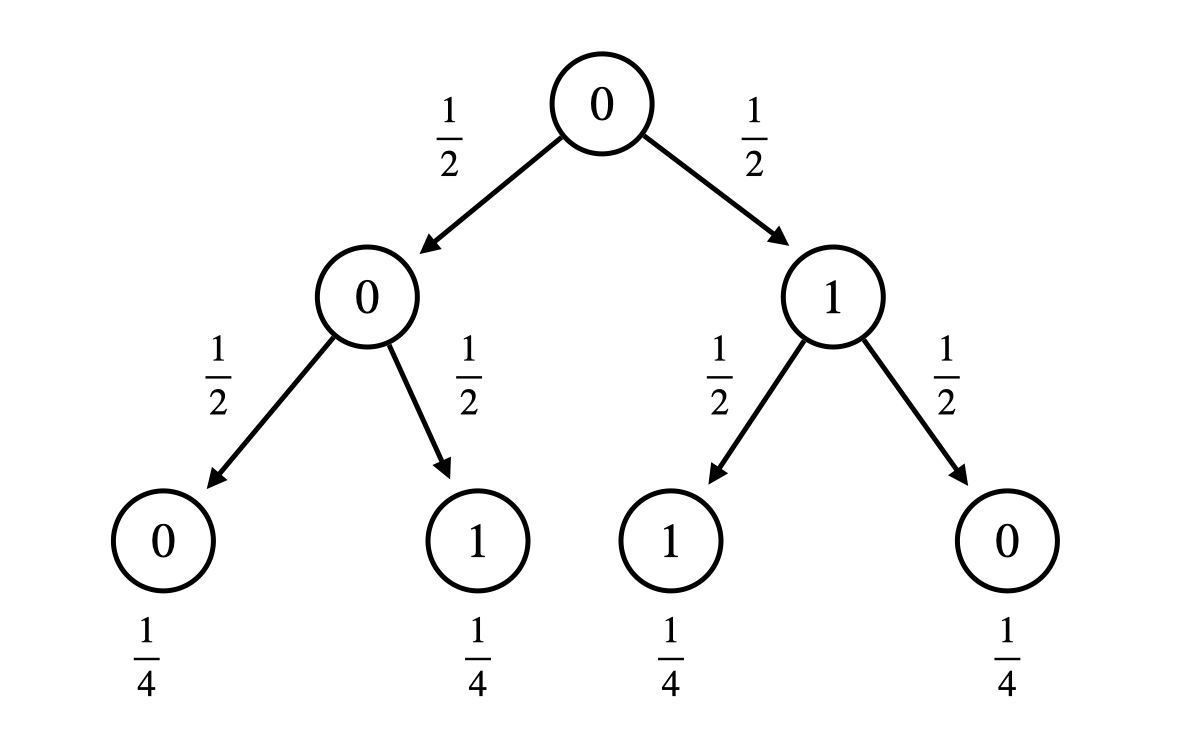
\includegraphics[width=0.5\textwidth]{src/ps_classical.jpeg}
\end{align}
where the numbers on the bottom line denote the total probability to end up in one of the four possible paths. The total probability assigned to each of the leaves in this binary tree is simply computed by walking the path from the root to the leaf and multiplying all probabilities on the way. To calculate the total probability to end up in one of the possible states (i.e. the bit is in 0 or 1) we just sum up the path probabilities that end up in the corresponding states -- therefore the name ``path sum''.\\
For the quantum process we can essentially create the sam path sum representation with just a slight change: now we use probability amplitudes instead of probabilities
\begin{align}
    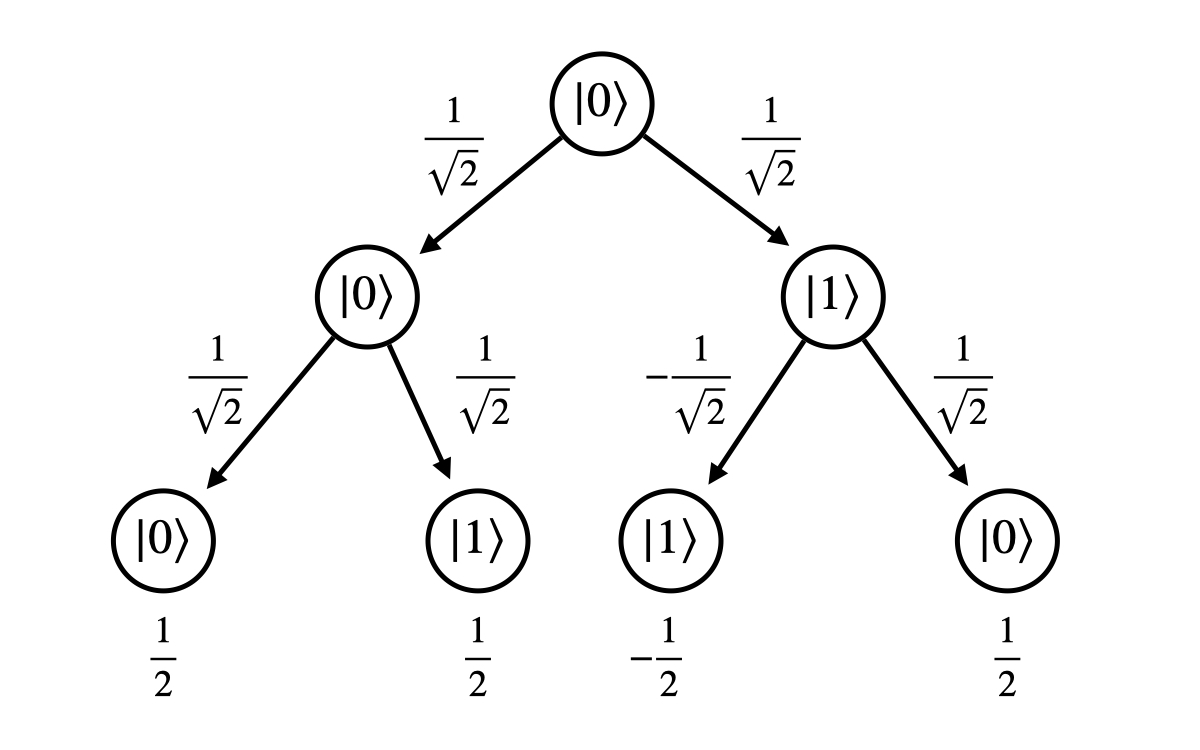
\includegraphics[width=0.5\textwidth]{src/ps_quantum.jpeg}
\end{align}
Now the numbers denoted under the leaves are the accumulated probability amplitudes (or short: path amplitudes) for the corresponding paths which are computed in the same manner, but simply multiplying all probability amplitudes on the corresponding path. 
The total probability amplitude for each of the states $\ket
{0}$ and $\ket{1}$ is then given by the sum of all path amplitudes with paths leading to the corresponding state. In this case, the total amplitude for $\ket{1}$ is $1/2 - 1/2 = 0$ so the state $\ket{1}$ will never be observed after the process.

\subsection{A First Quantum Algorithm}

\begin{def*}
\noindent\textbf{Deutsch Problem:} Take a Boolean function $f$ acting on a single bit. Determine if $f$ is constant, \textit{i.e.} if $f(0)=f(1)$.
\end{def*}

\begin{algo*}
\noindent\textbf{Classical Algorithm:} The algorithm is simple. We evaluate $f(0)$ and $f(1)$ and compare the results. In terms of oracle-complexity or ``query-complexity'' (``how often do we need to query the function $f$'') this needs two calls to $f$ (in all cases).
\end{algo*}

\paragraph{Quantum Algorithm:} 
The quantum algorithm is a bit more complex, but it manages to get away with a \textit{single call} to a quantum operation that contains the function $f$.\\
First, we need to define this quantum operation which shall act on the ``(computational) basis states'' (the quantum states that correspond to the classical bit states) as
\begin{def*}[Deutsch oracle]
\begin{align}
    U_f \ket{k} = (-1)^{f(k)} \ket{k}, \quad k \in \left\{0,1\right\}.
\end{align}
\end{def*}
This is a so-called ``phase-encoding'' which encodes the Boolean function $f$ that maps to $\left\{0,1\right\}$ into the values $\left\{+1,-1\right\}$ called``phases''.~\footnote{``phases'' can be general complex numbers on the unit circle, \textit{i.e.} all numbers $e^{-i\varphi }$ with $\varphi \in \mathbb{R}$. Of course the numbers $\pm 1$ are included. Sometimes the number $\varphi$ is also called phase.} 
Having defined the Deutsch oracle, the actual algorithm is almost complete
\begin{algo*}[\texttt{Deutsch} algorithm]
The Deutsch algorithm solves the Deutsch problem with a single query to the oracle $U_f$. The algorithm is the sequence of operations $\hd U_f \hd$ applied to a qubit in state $\ket{0}$.
\begin{align}
    U_D \ket{0} = \hd U_f \hd \ket{0} = \begin{cases}
        \pm\ket{0}, & f\text{ is constant}\\
        \pm\ket{1}, & \text{else}.
    \end{cases}
\end{align}
If $f$ is constant we have 100\% chance of reading out $\ket{0}$ while otherwise we will always read out $\ket{1}$.
\end{algo*}
Let's see how the algorithm works, by walking through the individual steps
\begin{align}
    U_D \ket{0} &= \hd U_f \hd \ket{0} = \hd U_f \ket{+}\nonumber\\
    &= \hd \frac{1}{\sqrt{2}}\left(U_f\ket{0} + U_f\ket{1} \right) \nonumber\\
    &= \hd \frac{1}{\sqrt{2}} \left((-1)^{f(0)}\ket{0} + (-1)^{f(1)}\ket{1}\right).
\end{align}
At this point, it makes sense to inspect the four possible cases.\\

\textit{case 1: $f(0)=f(1)=0$ (constant 0)} 
\begin{align}
    \hd \frac{1}{\sqrt{2}} \left((-1)^{f(0)}\ket{0} + (-1)^{f(1)}\ket{1}\right) = \hd \ket{+} = \ket{0}
\end{align}
\textit{case 2: $f(0)=f(1)=0$ (constant 1)} 
\begin{align}
    \hd \frac{1}{\sqrt{2}} \left((-1)^{f(0)}\ket{0} + (-1)^{f(1)}\ket{1}\right) = -\hd \ket{+} = -\ket{0}
\end{align}
note that we can ``pull'' the ``global minus'' sign to the front (this is just basic arithmetics).\\
\textit{case 3: $f(k)=k$ ($f$ is unit operation)} 
\begin{align}
    \hd \frac{1}{\sqrt{2}} \left((-1)^{f(0)}\ket{0} + (-1)^{f(1)}\ket{1}\right) = \hd \ket{-} = \ket{1}
\end{align}
\textit{case 4: $f(k)=\neg k$ ($f$ is negation)} 
\begin{align}
    \hd \frac{1}{\sqrt{2}} \left((-1)^{f(0)}\ket{0} + (-1)^{f(1)}\ket{1}\right) = -\hd \ket{-} = -\ket{1}
\end{align}
Note that the signs do not change the probability of reading out $\ket{0}$ or $\ket{1}$. 

In the same way as before, we can construct a path-sum representation
\begin{align*}
   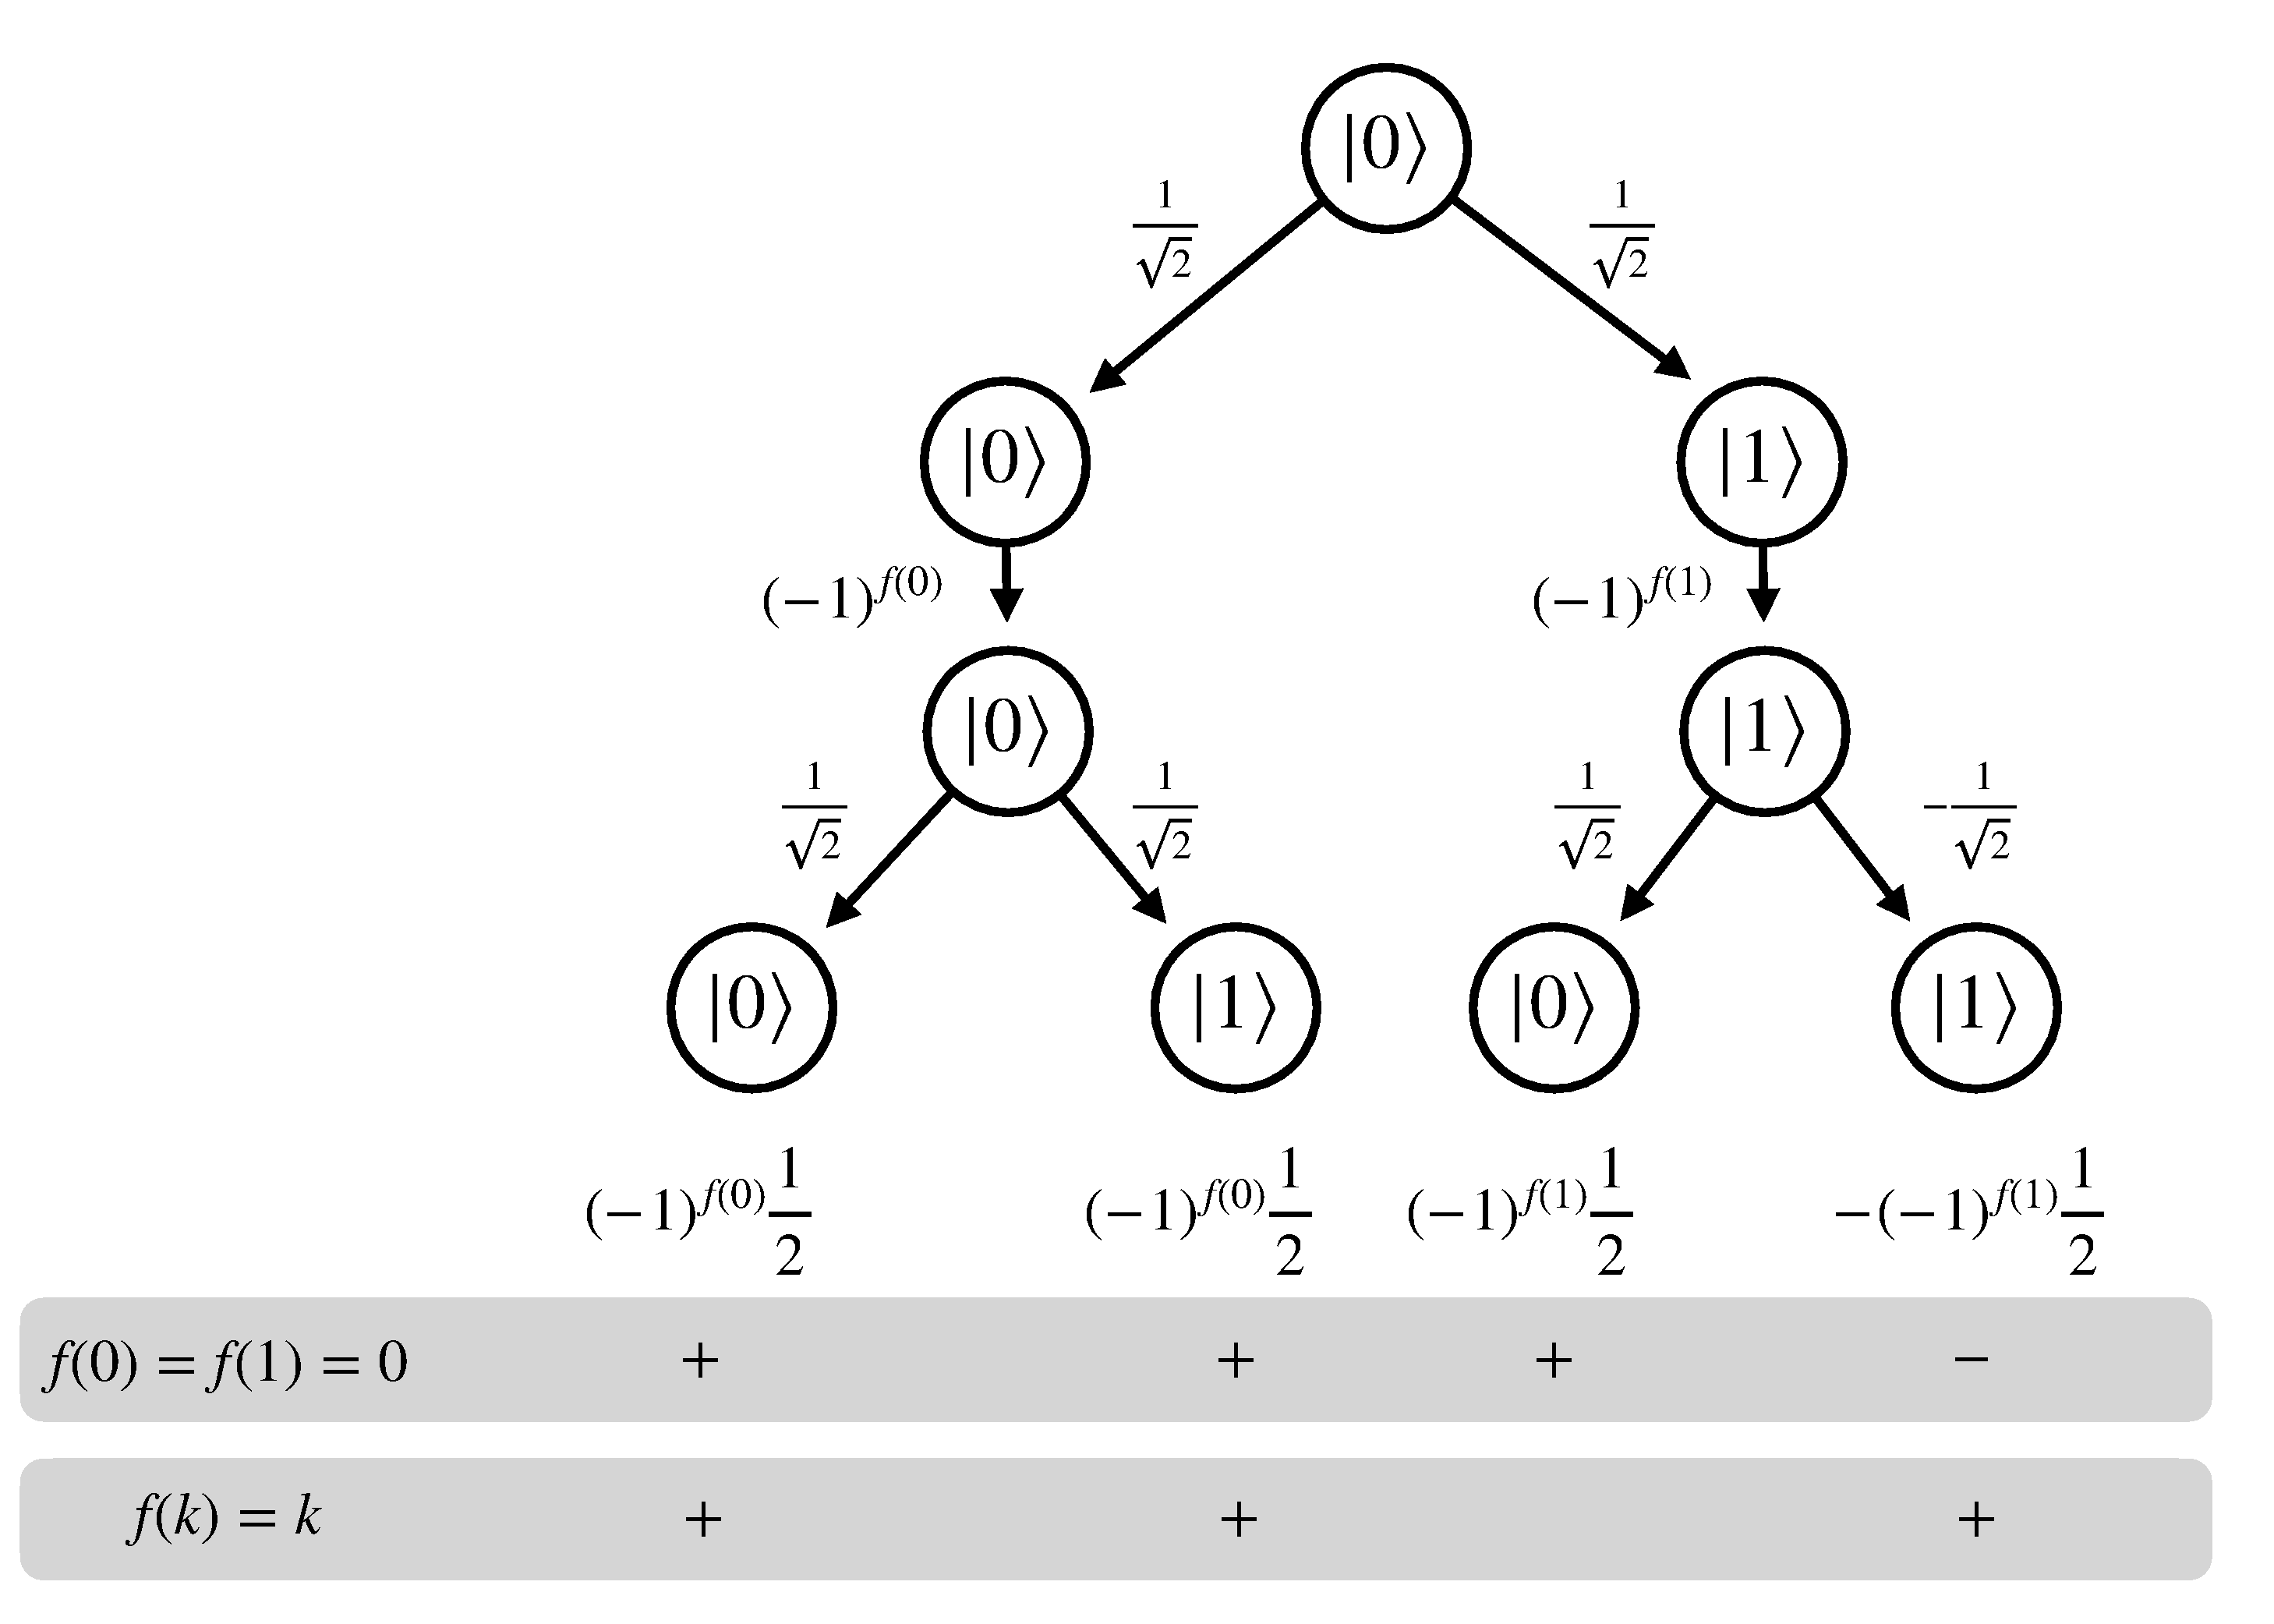
\includegraphics[width=0.75\textwidth]{src/deutsch-phase-oracle.pdf} 
\end{align*}
where we just indicate the signs of the amplitudes for two of the 4 possible $f$.



\subsection{Multi-Qubit Hadamard}
Before we start with the next example, it is useful to think about the action of Hadamard gates on multiple qubits.
A quantum state of multiple qubits can be written as a linear combination over all classical bit states (the ``computational basis states''). We can either label them as integers $\ket{\mathbf{k}}$ or by their explicit bit values $\ket{k_1k_2\dots k_N}$. Example for a 3 qubit basis states: $\mathbf{0}=000, \mathbf{1} = 001, \mathbf{2}=010, \dots ,\mathbf{5} = 101, \dots$. 
Often it can be useful to use the symbol $\otimes$ as a separator to indicate the individual qubits. Take for example
\begin{align}
    \ket{1011} = \ket{1}\otimes\ket{011} = \ket{10}\otimes\ket{11} = \ket{1}\otimes\ket{0}\otimes\ket{1}\otimes\ket{1}.
\end{align}
We can do this in the same way for operations. Take for example a 3 qubit system where we want to act with the Hadamard operation on the second qubit, we can denote this either by indicating the qubit onto which the operation acts in parentheses or explicitly using the $\otimes$ symbol
\begin{align}
    \hd(2) = 1 \otimes \hd \otimes 1.
\end{align}
If we are acting with $N$ Hadamard operations on $N$ qubits respectively, we can also use the short-notation
\begin{align}
    \hd^{\otimes N} = \hd(1) \hd(2) \dots \hd(N) = \bigotimes_{k=1}^{N} \hd =  \hd \otimes \hd \otimes \dots \otimes \hd.
\end{align}
A graphical notation -- a quantum circuit -- would be\\

\begin{center}
    $\hd^{\otimes 3}$ = \begin{quantikz}
& \gate{H} &[1cm]&\\
& \gate{H} &[1cm]&\\
& \gate{H} &[1cm]&\\
\end{quantikz}
\end{center}


where the wires represent the qubits and the boxes the operations. Note that quantum circuits are read from left to right.

In the same way, we can write for states
\begin{align}
    \ket{\mathbf{0}} = \ket{0}^{\otimes N} = \bigotimes_{k=1}^{N}\ket{0} = \ket{00\dots 0}
\end{align}
These are just different notations for the same thing. Depending on the context their usefulness will change.
Take for example $\hd \otimes \hd$, we know that this is a two-qubit operation, where a Hadamard operations will act on each qubit. In cases where we don't need explicit labels, this is convenient notation. If we need explicit labels, e.g. a Hadamard acting on qubit 3 and one on qubit 5 in a set of $N$ qubits, then $\hd(3) \hd(5)$ is more compact than $1\otimes 1 \otimes \hd \otimes 1 \otimes \hd \otimes 1 \otimes \dots \otimes 1 $
Now we can start to think about the action of such a collection of Hadmard gates on $N$ qubits.\\

Take $N$ qubits and let $N$ Hadamard gates act on each of them 
If acting on a $N$ bit basis state (a classical state corresponding to all $N$ bits being in either 0 or 1) we get
\begin{align}
    \hd^{\otimes N} \ket{k_1k_2\dots k_N} &=  \bigotimes_{i=1}^{N} \hd\ket{k_i} \nonumber\\ &= \bigotimes_{i=1}^{N} \frac{1}{\sqrt{2}}\left(\ket{0} + \left(-1\right)^{k_i} \ket{1} \right) \nonumber\\&=\frac{1}{\sqrt{2^N}} \sum_{l=0}^{2^N-1} \left(-1\right)^{\left(\sum_{i=1}^N k_il_i\right)} \ket{l_1 l_2\dots l_N}
\end{align}
If we introduce the shortcut 
\begin{def*}[bitwise dot-product]
\begin{align}
    \mathbf{l} \odot \mathbf{k} = l_1 k_1 \oplus l_2k_2 \oplus \dots \oplus l_N k_N
\end{align}
\end{def*}
for the bitwise dot-product between the $N$-bit binary representation of two integers $l$ and $k$, we can write
\begin{def*}[Hadamard basis]
\begin{align}
    H^{\otimes N} \ket{\mathbf{k}} = \frac{1}{\sqrt{2^N}} \sum_{\mathbf{l}=0}^{2^N-1} \left(-1\right)^{\mathbf{k}\odot \mathbf{l}} \ket{\mathbf{l}}.
\end{align}
\end{def*}
It is useful to verify this formula for yourself (ideally after you have gained some experience with these types of calculations), but for now, it is also fine to just use it.\\
Three important observations that we need later
\begin{highlight}
\begin{enumerate}
    \item if $\mathbf{k}=\mathbf{0}$ then all negative signs vanish from the right-hand-side.
    \item if $\mathbf{k}\neq\mathbf{0}$ then there will always be negative signs on the right-hand-side. On closer inspection: half of the $2^N$ basis states will get a negative sign.
    \item the states on the right-hand-side will be transformed into computational basis states when we act with a sequence of Hadamard operations on them (since Hadamards are self-inverse)
\end{enumerate}
\end{highlight}
\subsection{Deutsch-Jozsa}
A straightforward extension of the \texttt{Deutsch} algorithm is the algorithm by Deutsch and Jozsa. 
It has the same premise, but will lead to a (formal) exponential separation between classical and quantum realizations (again with respect to the number of queries to either the classical function $f$ or the quantum operation encoding $f$).\\
Starting from the Deutsch Problem that was asking if a Boolean function on a single bit is constant, we can go one step further and consider Boolean functions $f$ of $N$ bits. 
Here we will now ask if the function $f$ is constant ($\forall k: f(k) = x$ with constant $x\in\left\{0,1\right\}$ and $k$ being one of the $2^N$ possible assignments of the $N$ bits) or \textit{balanced}. The second states that for exactly half of the possible input bitstrings the function will evaluate to 0 and for the other half to 1. We can view this as a so-called ``promise Problem'', we ask if the function is constant, but we have the promise that the function is either constant of balanced.

\begin{def*}
\textbf{Deutsch-Jozsa Problem:} Given an $N$ bit Boolean function promised to be either constant or balanced, determine if its constant.
\end{def*}

\begin{algo*}
\textbf{Classical Algorithm:} We evaluate the function on $2^N/2+1$ different input states. If they all result in the same output, the function is constant, otherwise it's balanced (this is the promise). This has an exponential runtime in the number of calls to $f$.
\end{algo*}

\begin{algo*}[\texttt{Deutsch-Jozsa}]
As before, the algorithm is a bit more complicated, but a single call to $U_f$ will suffice!
The quantum operation is constructed similar to $U_\text{D}$ from \texttt{Deutsch}
\begin{align}
    U_\text{DJ} = \hd^{\otimes N} U_f \hd^{\otimes N} 
\end{align}
with the oracle $U_f$ acting as
\begin{align}
    U_f \ket{\mathbf{k}} = (-1)^{f(\mathbf{k})}\ket{\mathbf{k}}.
\end{align}
The algorithm applies $U_{\text{DJ}}$ on $N$ input qubits, all initialized to the $\ket{0}$ state
\begin{align}
         {U}_\text{DJ} \ket{\boldsymbol{0}} &= \begin{cases}
         \pm \ket{\mathbf{0}}, & f \text{ is constant}\\
         \pm \ket{\mathbf{k}}, \mathbf{k}\neq \mathbf{0} & f \text{ is balanced}
     \end{cases}
\end{align}
A single query to $U_f$ (contained in $U_\text{DJ})$ is sufficient to solve the problem.
\end{algo*}
As a quantum circuit, \texttt{Deutsch-Jozsa} (here for $N=3$) takes the form
\begin{center}
$ U_\text{DJ}$ = \begin{quantikz}
& \gate{H} & \gate[3]{U_f}& \gate{H} \\
& \gate{H} &[1cm] & \gate{H}\\
& \gate{H} &[1cm] & \gate{H}\\
\end{quantikz}
\end{center}
 Acting on $N$ qubits in the zero state we have
 \begin{align}
      {U}_\text{DJ} \ket{0}^{\otimes N} &= \frac{1}{\sqrt{2^N}} \hd^{\otimes N}\sum_{k=0}^{2^N-1} {U}_f \ket{\mathbf{k}}\nonumber \\
      &= \frac{1}{\sqrt{2^N}} \hd^{\otimes N}\sum_{k=0}^{2^N-1} (-1)^{f(\mathbf{k})}\ket{\mathbf{k}}.
 \end{align}
 If $f(\mathbf{k})$ is constant, either have $f\mathbf{(k)}=1$ or $f({\mathbf{k}})=0$ in all case this will, after application of the remaining Hadamard operation (see observation 1 above), lead to either $\pm\ket{0}^{\otimes N}$ where the choice of $\pm$ will depend on the value that $f=const$ takes. The sign has however no impact on the probability to read out the state $\ket{0}^{\otimes N}$ (all qubits in state $\ket{0}$) which is 100\% in this case.
 If $f$ is balanced on the other hand, then half of the signs will be negative, which will lead to a basis state $\ket{\mathbf{k}}$ with $\mathbf{k}\neq 0$ after the final Hadamard operations are applied (see observation 2 above).\\
 In summary we arrive at
 \begin{align}
     {U}_\text{DJ} \ket{0}^{\otimes N} &= \begin{cases}
         \pm \ket{\mathbf{0}}, & f \text{ is constant}\\
         \pm \ket{\mathbf{k}}, \mathbf{k}\neq \mathbf{0} & f \text{ is balanced}
     \end{cases}
 \end{align}

 \paragraph{Exponential Speedup:} \texttt{Deutsch-Jozsa}  has an exponential speedup when we compare the quantum algorithm: only a \textit{single} query to $U_f$ is necessary, while classically we require $2^N/2 + 1$ queries to $f$. These are exponentially more queries in the classical counterpart.\\
On a second look we do however realize that this exponential speedup only holds if we compare with a deterministic classical strategy with 100\% certainty. We can ask ourselves: What if, we only sample $M$ of the possible $2^N$ inputs to $f$. Assume for now that $f$ is not constant, we evaluate $f$ on one of the possible inputs (let's say $f(0000...0)=x$), you can call this a ``gauge query'' because now we need only ask for each new query if it will reach the same value $x$. With each sample of the possible inputs we have a 50\% chance to get an input $k$ that leads to $f(k)\neq x$, at this point, we know for sure that $f$ is not constant. The chances of sampling a $k$ with this property are always $1/2$, so on average we will arrive at $2$ queries~\footnote{details not important here; see info3 lecture on average case analysis. This example is basically the same} to $f$ in order to determine that $f$ is not constant (in total we have then 3 queries, counting the gauge query as well). In the case where $f$ is constant, the argument is the same, just with insecurity about the current assumption that $f$ is constant.
All in all, the speed-up shrinks basically down to the original Speedup of a factor of 2 (plus one gauge query). 

\subsection{Bernstein-Vazirani}
A slight modification of Deutsch-Jozsa leads to the \texttt{Bernstein-Vazirani} algorithm. Here we can show a polynomial improvement (from linear to constant) in the number of queries when comparing the quantum algorithm with the best possible classical algorithm. 

\begin{def*}[Bernstein-Vazirani problem]
    Given is a Boolean function $f$ acting on $N$ bits with the promise that $f(\mathbf{x}) = \mathbf{x}\odot \mathbf{y} =  x_1y_1 \oplus x_2y_2 \oplus \dots \oplus x_Ny_N$ (bit wise binary dot-product) with an unknown $N$-bit string $\mathbf{y}$. The task is to find $\mathbf{y}$.
\end{def*}

\begin{algo*}[Classical solution]
    Classically we can query $f$ with the $N$ ``unary'' bitstrings $\mathbf{x}_1 = 000\dots 01, \mathbf{x}_2 = 000\dots 10, \dots, \mathbf{x}_N = 100\dots 00$. Each query will reveal one bit of $\mathbf{y}$ via $f(\mathbf{x}_i) = \mathbf{x}_i \odot\mathbf{y} = y_i$. So we need exactly $N$ queries to determine $\mathbf{y}$ and we can not get away with less.
\end{algo*}

\begin{algo*}[\texttt{Bernstein-Vazirani}]
We perform the \texttt{Deutsch-Jozsa} operation where $U_f$ encodes the $f$ from the Bernstein-Vazirani problem to the all-zero state
    \begin{align}
         {U}_\text{DJ} \ket{\mathbf{0}} &= \ket{\mathbf{y}}
\end{align}
the resulting state is the sought bitstring $\mathbf{y}$ which can now just be read-out from the qubit register.  
We just need a single query to $U_f$ to get the answer with 100\%.
\end{algo*}
To see that this is actually true:
\begin{align}
U_\text{DJ}\ket{\mathbf{0}} &= \hd^{\otimes N} U_f \hd^{\otimes N}\ket{\mathbf{0}} \nonumber\\
&= \hd^{\otimes N} \frac{1}{\sqrt{2^N}} \sum_{k=0}^{2^N-1} U_f\ket{\mathbf{k}} \nonumber\\
&= \hd^{\otimes N} \frac{1}{\sqrt{2^N}} \sum_{k=0}^{2^N-1} (-1)^{\mathbf{k}\odot \mathbf{y}}\ket{\mathbf{k}}\nonumber\\
&= \ket{\mathbf{y}}
\end{align}
Where we have used observation 3 from above in the last step. Note that the only thing that changed w.r.t to \texttt{Deutsch-Jozsa}  is the promise on $f$.\\

The polynomial separation that we are seeing here between classical and quantum is not bad, but it can actually be improved to achieve an exponential separation w.r.t queries to $U_f$ and $f$ for specifically constructed decision problems within BQP (the quantum analog of P) and BPP (the probabilistic analog of P). We will skip the details here.
\clearpage

\subsection{Summary}
First encounters with key concepts in quantum information processing:
\begin{itemize}
    \item wavefunctions
    \item interference
    \item linear operators 
    \item probability amplitudes
    \item qubits
    \item the \textsc{hadamard} operation
    \item path sum representations
\end{itemize}


We have also seen examples of quantum Algorithms that have advantages over classical algorithms with respect to query complexity
\begin{enumerate}
    \item \texttt{Deutsch}: single query (quantum) vs two queries (classical)
    \item \texttt{Deutsch-Jozsa}: single query (quantum) vs $\Theta(2^N)$ queries (cassical) -- if we tolerate small errors we will however get away with $3$ queries on average.
    \item \texttt{Bernstein-Vazirani}: single query (quantum) vs $N$ queries (classical)
\end{enumerate}

We also observe here that the proven speedups are only with respect to query complexity. Meaning that the ``oracle'' $U_f$ is already given to you. With the exception of the plain \texttt{Deutsch} algorithm, the speedup also just works because we are given a promise (constant or balanced, or the promise that the Boolean function has a specific structure).\\



%\clearpage
% \section{The Hidden Subgroup Problem}

\subsection{Simon's Problem}
Simon's problem is on first glance similar to the problem of Bernstein and Vazirani. Again, we are dealing with an oracle in the form of a function on $N$ bits and a hidden $N$-bitstring $\mathbf{y}$. 
The first difference: the function $f$ is not mapping to a single bit, but can map to many
\begin{align}
    f: \left\{0,1\right\}^N \rightarrow \left\{0,1\right\}^M,\;\; M\leq N
\end{align}
The oracle $f$ promises
\begin{align}
    \forall \mathbf{x} \neq \mathbf{x}': f(\mathbf{x}) = f(\mathbf{x}') \Leftrightarrow \mathbf{x}' = \mathbf{x} \oplus \mathbf{y}
\end{align}
and the task is to find the \textit{hidden} bitstring $\mathbf{y}$.\\

A classical algorithm to the problem would be
\begin{enumerate}
    \item Select a pair $\mathbf{x},\mathbf{x'}$ (at random).
    \item evaluate $f(\mathbf{x})=f(\mathbf{x')}$, if true keep the pair.
    \item repeat until $M$ pairs are found.
    \item The $M$ pairs $\left(\mathbf{x}_k,\mathbf{x}'_k\right)$ provide enough information to solve the linear system $\mathbf{x}_k = \mathbf{x}'_k \oplus \mathbf{y}$ and determine $\mathbf{y}$.
\end{enumerate}
The problem with efficiency is, that, in the worst-case, we need to sample an exponential amount of pairs (leading to exponentially many queries to $f$). The quantum version allows us to find $M$ pairs with a linear amount of queries. An average case analysis improves things classically, but remains exponential, we will not bother with this here.\\

\begin{def*}[Simon's Problem]
We are given a function $f:\left\{0,1\right\}^N \rightarrow \left\{0,1\right\}^M$ with
$$ f(\mathbf{x}) = f(\mathbf{z}) \Leftrightarrow \mathbf{x} \oplus \mathbf{y} = \mathbf{z}$$
for all $\mathbf{x}\neq \mathbf{z}$ and unique hidden $N$-bitstring $\mathbf{y}\in\left\{0,1\right\}^N$ that has to be found.
\end{def*}

We can already recover a special case: If $\mathbf{y}=\mathbf{0}$ then $\mathbf{x} = \mathbf{x}' \oplus \mathbf{y}$ holds true for \textit{all} pairs $(\mathbf{x}, \mathbf{x}')$, therefore $f(\mathbf{x})=f(\mathbf{x}')$ has to hold for all pairs as well making $f$ constant.~\footnote{Note however, that we can not simply run \texttt{Deutsch-Josza} to identify this case, since after a single run that results in a positive answer, we can not be sure, if the probability was 100\%. The Algorithm needs to be adapted a little, and we will require multiple queries to it, in order to recover $\mathbf{y}$.}
On the other hand, if the hidden string is not the zero-string, $\mathbf{y}\neq 0$, then the function needs to have $2^N/2$ distinct values: one for each pair $\mathbf{x}, \mathbf{x}\oplus \mathbf{y}$.~\footnote{proof: for $\mathbf{a} \neq \mathbf{b} \oplus \mathbf{y}$ assume $f(\mathbf{a})=f(\mathbf{b})$ then it follows from the promised structure $\mathbf{a} = \mathbf{b} \oplus \mathbf
y$ which is a contradiction. At the same time, if we have $\mathbf{a} = \mathbf{a}' \oplus \mathbf{y}$ we can not have a second $\mathbf{a} = \mathbf{a}'' \oplus \mathbf{y}$ because  $\mathbf{a}  = \mathbf{a}' \oplus \mathbf{y}= \mathbf{a}'' \oplus \mathbf{y} \Rightarrow \mathbf{a}'=\mathbf{a}''$ }\\
We can summarize the promised properties of the function $f$ as
\begin{align}
&f(\mathbf{x}) = f(\mathbf{x} \oplus \mathbf{y})\\
&\mathbf{y}\neq\mathbf{0} \Rightarrow f(\mathbf{x}) \neq f(\mathbf{z})\; \; \forall \mathbf{z} \notin \left\{\mathbf{x}, \mathbf{x}\oplus \mathbf{y}\right\}\\
&\mathbf{y}=\mathbf{0} \Rightarrow f=\text{const}
\end{align}


The algorithm works with two registers, one carrying the input of $f$ and one the output. We assume that the operation $f$ is available as unitary operation $U_f$ acting on these registers as
\begin{align}
    U_f \left(\ket{\mathbf{x}}\otimes \ket{\mathbf{0}}\right) = \ket{\mathbf{x}}\otimes \ket{ f(\mathbf{x})}.
\end{align}
The full algorithm is
\begin{algo*}[\texttt{Simon}{'s Algorithm}]
Execute the circuit
\begin{center}
$ U_\text{S}$ = \begin{quantikz}
& \gate{\hd^{\otimes N}} & \gate[2]{U_f}& \gate{\hd^{\otimes N}} & \qw \\
& \qw  &[1cm] & \qw & \qw\\
\end{quantikz}
\end{center}
and keep the results on the first register. Repeat $O(N)$ times until enough bitstrings $\mathbf{k}$ are sampled to solve the linear system $\mathbf{y}\odot \mathbf{k}=0$.
\end{algo*}
We begin (at this point, almost traditionally) with a sequence of Hadamard gates on each qubit in the first register followed by the oracle $U_f$ acting on both
\begin{align}
    \ket{\mathbf{0}}\otimes \ket{\mathbf{0}} \xrightarrow[]{\hd^{\otimes N}} \ket{+}^{\otimes N} \otimes \ket{\mathbf{0}} = \frac{1}{\sqrt{2^N}}\left(\sum_{k=0}^{2^N-1}\ket{\mathbf{k}}\right) \otimes \ket{\mathbf{0}} \xrightarrow[]{U_f} \frac{1}{\sqrt{2^N}} \sum_{k=0}^{2^N-1} \left(\vphantom{\sum_{\suum}}\ket{\mathbf{k}}\otimes \ket{{f(\mathbf{k})}}\right).\nonumber
\end{align}
After the state is prepared, we read out the second qubit register -- that is, we will get one of the possible values of $f(\mathbf{k})$, let's call them $a = f(\mathbf{i})$, with $\mathbf{i}\in \left\{\mathbf{k}\right\}_{k=0}^{2^N-1}$ and probability of $1/2^N$ for each of them. As a result the remaining qubit register collapses to a linear combination of $\mathbf{i}$ and the partner $\mathbf{i}\oplus \mathbf{y}$ that lead to $f(\mathbf{i})=a$
\begin{align}
    \frac{1}{\sqrt{2}} \left( \ket{\mathbf{i}} + \ket{\mathbf{i\oplus y}}\right),
\end{align}
At this point we do not profit yet, from reading out the first register, we first need to transform again with a Hadamard operation on all qubits on the remaining register
\begin{align}
        \frac{1}{\sqrt{2}} \left( \ket{\mathbf{i}} + \ket{\mathbf{i \oplus y}}\right) \xrightarrow[]{\hd^{\otimes N}}& \frac{1}{\sqrt{2}}\left( \left(\frac{1}{\sqrt{2^N}}\sum_{k=0}^{2^N-1} (-1)^{\mathbf{k}\odot \mathbf{i}}\ket{\mathbf{k}}\right) +\left(\frac{1}{\sqrt{2^N}}\sum_{k=0}^{2^N-1} (-1)^{\mathbf{k}\odot( \mathbf{i}\oplus\mathbf{y})}\ket{\mathbf{k}}\right) \right)\nonumber\\
        &= \frac{1}{\sqrt{2^{N+1}}}\sum_{k=0}^{2^N-1} (-1)^{\mathbf{k\odot i}} \left(1+(-1)^{\mathbf{k}\oplus \mathbf{y}}\right) \ket{\mathbf{k}} \nonumber\\
        & = \frac{1}{\sqrt{|A|}} \sum_{k\in A^\perp} (-1)^{\mathbf{k\odot i}} \ket{\mathbf{k}}, \quad A^\perp = \left\{\mathbf{k} \;|\; \mathbf{k} \odot \mathbf{y} = 0\right\}.
\end{align}
This is where the magic happened. If we are now reading out the register, we will get a $\mathbf{k}$ such that $\mathbf{k\odot \mathbf{y}}=0$ (with uniform probability over all such candidates). This is completely independent from what value $a=f(\mathbf{i})$ we have read out before. To determine the $M$-bitstring $\mathbf{y}$ via the linear system $\mathbf{k\odot \mathbf{y}}=0$ it suffices to get $M$ candidates $\mathbf{k}$. So we need to repeat the algorithm $O(M)$ times to solve the problem. While doing this, we can also detect the special case $f=const$ with high probability (we would read out the same value in the first register on every trial and the second register would always give back $\mathbf{0}$).
To digest this information, it is beneficial to look at a concrete example.

\paragraph{Example: $N=2,M=1,\; f(\mathbf{x})=x_1\oplus x_2$}: In this example our function acts on two qubits with the concrete assignments $00\rightarrow 0, 01\rightarrow 1, 10 \rightarrow 1, 11 \rightarrow0$. So we have $f(\mathbf{0})=f(\mathbf{3})$ and $f(\mathbf{1})=f(\mathbf{2})$ and the hidden string is $\mathbf{y}=\mathbf{3}=11$. From all possible 4 combination of two bits, two (00 and 11) fulfill the equation $\mathbf{y} \odot \mathbf{k} = y_1k_1 \oplus y_2k_2 = k_1 \oplus k_2=0$. The quantum circuit prepares the states
\begin{align}
    \ket{0}^{\otimes}\otimes \ket{0} \xrightarrow[]{\hd^{\otimes N}}& \frac{1}{2}\left(\ket{00} + \ket{01} + \ket{10} + \ket{11}\right)\otimes \ket{0}\\
    \xrightarrow[]{U_f}& \frac{1}{2} \left(\ket{00}\otimes\ket{0} + \ket{01}\otimes\ket{1} + \ket{10}\otimes \ket{1} + \ket{11}\otimes \ket{0}\right)\nonumber\\
    \xrightarrow[]{\hd^{\otimes N}}& \frac{1}{2} \left(\ket{++}\otimes\ket{0} + \ket{+-}\otimes\ket{1} + \ket{-+}\otimes \ket{1} + \ket{--}\otimes \ket{0}\right)\nonumber\\
    &= \frac{1}{\sqrt{2}}\left(\left(\ket{00} + \ket{11}\right)\otimes\ket{0} + \left(\ket{00} + \ket{11}\right)\otimes\ket{1}\right)\nonumber\\
    & =\frac{1}{\sqrt{2}}\left(\ket{00} + \ket{11}\right)\otimes\ket{+}.
\end{align}
So by reading out the first two qubits we either get $00$ or $11$, the two candidates we need to determine $\mathbf{y}$ via the linear system $\mathbf{y}\odot \mathbf{k}=0$. Note again that the end result is independent of the third qubit.
At this point we also realize, that reading out the second register (that holds the value of $f$ after applying the oracle) is actually not necessary. 
\subsection{Groups and their Properties}

A group is an algebraic structure that obeys the axioms
\begin{def*}[(Abelian) Group $(G,\odot)$]\phantom{...}\\
A set of elements $G = \left\{e_k\right\}_{k=1}^N$ with group action $\odot: G\times G
\rightarrow G $ and axioms
\begin{align*}
    &a,b,c\in G: (a\odot b)\odot c = a\odot (b\odot c)& \text{associativity}\\
    &\exists e\in G, \forall g\in G:  e\odot g = g\odot e = g &\text{neutral element}\\
    &\forall g\in G, \exists g^{-1}\in G: g\odot g^{-1}= g^{-1}\odot g = e & \text{inverse element}
\end{align*}
If additionally the group action commutes
\begin{align}
    \forall a,b\in G: a \odot b = b\odot a
\end{align}
the group is called \textit{abelian}
\end{def*}
Note that we used $\odot$ as a group action and not as a binary inner product to follow standard notation. If we are dealing with a concrete realization or a \textit{representation} of a group, we replace $\odot$ with the corresponding symbol that is most suitable (e.g. $\odot \rightarrow +$ if we are using addition of numbers.\\
The usual examples are: 
\begin{itemize}
    \item $(\mathbb{Z},+)$ (integers under addition)
    \item $(\mathbb{C}^{N\times M}, +)$ (matrices under addition)
    \item $(\text{Herm}(N),+)$ (Hermitian $N\times N$ matrices under addition)
    \item $(U(N), \cdot )$ (Unitary $N\times N$ matrices under matrix-multiplication)
\end{itemize}
which are, except for the last one, all abelian.
To test your understanding of the notion of a group: show that $(\mathbb{Z},\cdot)$, $(\mathbb{R}, \cdot)$ and $(\mathbb{N}, +)$ are not groups and explain why general matrices under matrix multiplication do not form a group.\\

Prominent Abelian groups are the cyclic groups that can be represented by integers with modular addition or rotations in vector spaces.
\begin{def*}[Cyclic Group]
The cyclic group $C_n$ is an abelian group of $n$ elements $C_n = \left\{g_0,g_1,g_2,g_3,\dots g_{n-1}\right\}$ with
\begin{align}
    &g_0\odot g_k = g_k & \text{neutral element}\\
    &g_1 \odot g_k = g_{(k\oplus_n1) } & \text{cyclic property}
\end{align}
where $\oplus_n$ denotes addition modulo $n$.
The element $g_1$ is called the \textit{generator} of the cyclic group and a typical notation is $G=\left\{e,g,g^2,g^3,\dots, g^{n-1}\right\}$.
\end{def*}
This is indeed a group: the inverse element of $g^k$ is $g^{n-k}$, since the neutral element is $e=g^0=g^n$. The typical example of a representation of $C_n$ is $\mathbb{Z}/n\mathbb{Z}$ integers with addition modulo $n$. 
A single bit is a realization of the group $C_2$ with $(\left\{0,1\right\},\oplus)$, two bits form the group $\left(\left\{0,1,2,3\right\}, \oplus_3\right)$. 
If we use bitwise binary addition, denoted as a simple $\oplus$, we have further examples for groups: $(\left\{\mathbf{0},\mathbf{1},\mathbf{2},\mathbf{3}\right\}, \oplus)$~\footnote{e.g. $\mathbf{1}\oplus\mathbf{3} = (0,1)\oplus(1,1) = (0\oplus 1, 1\oplus 1) = (1,0) = \mathbf{2}$} or more general $(\left\{\mathbf{k}\right\}_{k=0}^{2^N-1}, \oplus)$ we have a group with neutral element $\mathbf{0}$ and self-inverse elements. On first glance this doesn't appear to be a cyclic group, and it isn't, but it is isomorphic to the direct product of $N$ cyclic $C_2$ groups: $C^N_2:=C_2\times C_2\times \dots \times C_2$.\\
To continue with the quantum algorithms we unfortunately still need some vocabulary.

\begin{def*}[Subgroup]\phantom{...}\\
A subgroup $A\leq G$ of a group $(G,\odot)$ is a subset $A\subseteq G$ of the group elements such that $(A,\odot)$ is a group. Trivial subgroups are $A=\left\{e\right\}$ and $A=G$. The 
\end{def*}
Examples: The groups $(\mathbb{Z}, +)$ has no non-trivial subgroups. The group $(\text{Herm}(N), +)$ is a subgroup of $(\mathbb{C}^{N\times M}, +)$. The group $SU(N): \left\{e\in U(N)\;|\; \det(e)=1\right\}$ is a subgroup of $U(N)$ and each set of bitstrings with $M\leq N$ set to $0$ is a subgroup of $C_2^N$.\
\begin{def*}[Generating Set]\phantom{...}\\
A generating set $S\subseteq G$ of a group $(G,\odot)$ has the property
\begin{align*}
    \forall g\in G:  g=s_1\odot s_2\odot \dots \odot s_M
\end{align*}
with finite $M$ and $s_k\in S$ or $s_k^{-1}\in S$.
Meaning every element of the group can be generated by a finite combination of generating elements under the group action. If $S$ generates $G$ we write $G = \langle S\rangle $.
\end{def*}
Example: The notion of a generating set gives us an alternative definition of cyclic groups: the groups that can be generated by a single element $C_n = \langle \left\{g\right\}\rangle $ but also $C_n = \langle g^2\rangle$ and so on. The group of integers under addition  $(\mathbb{Z}, +)=\langle \left\{1\right\}\rangle $ is generated by a single element.~\footnote{the neutral element is for example generated via $0=1-1$, since the inverse of the generating elements can be used as well. In the same way, we can generate the negative numbers.} A generating set for the group $(\mathbb{R}, +)$ is the set $S=(0,1)\subset \mathbb{R}$ since for any  $x\in \mathbb{R}$ we can chose a $n\in \mathbb{N}$ such that $x/n<1$ meaning that $s=x/n\in S$ if we add this number $n$ times, we get $x$ back: $x=nx/n=ns=s+s+s+\dots +s$. This construction works for every $x\in \mathbb{R}$ and there are always finitely many additions: so we have a generating set.
\begin{def*}[Annihilator]\phantom{...}\\
The annihilator of a subgroup $A\leq G$ of an abelian group $G$ is defined as
\begin{align}
    A^\perp := \left\{g\in G \mid \forall a\in A :\chi_g(a)=1\right\}.
\end{align}    
\end{def*}
The annihilator~\footnote{naming is horrible in this context ... sorry} collects all elements whose characters are 1 for the operations in the respective subgroup. The annihilator itself is also a subgroup $A\leq G \Rightarrow A^\perp \leq G$.~\footnote{this is \textit{not} the case for non-abelian groups which also is one of the reasons why we are restricting ourselves here to abelian groups.}

\subsection{Fourier Transforms on Groups}

\begin{def*}[Representation of a Group] \phantom{...}\\
A map $f: G \rightarrow GL(V)$ that maps elements of a group $(G,\odot)$ to linear operators on the vector space $V$ such that the group action is preserved under the linear operators
\begin{align*}
    &c=a\odot b \Rightarrow f(c)=f(a)f(b) 
\end{align*}
is called a representation of the group $G$ on $V$. 
\end{def*}
In other words, the representation is a homomorphism~\footnote{homo (same) morph (form): this essentially means structure preserving} of the group onto linear operators of a vector space. Note that the preservation of the group action also preserves neutral and inverse elements
\begin{align*}
f(a^{-1}) &= f(a)^{-1}\\
    f(e) &= 1.\\
\end{align*}
Some examples:
The cyclic group $C_4$ is fully characterized over the abstract elements $(\left\{e,g,g^2,g^3\right\}, \odot)$ where $g^3 = g\odot g \odot g$ and $g^3\odot g=e$. If we write $C_4=(\left\{0,1,2,3\right\},\oplus_4)$ its not a representation in the sense of the definition, but rather a realization of the group with numbers (we did not map it to linear operators). A one-dimensional representation $f:C_4 \rightarrow GL(\mathbb{C})$ can be realized as mapping to the one-dimensional matrices (which are just numbers) acting on the one-dimensional vector space of complex numbers
\begin{align}
    \left\{e,g,g^2,g^3\right\} \mapsto \left\{1,i,-1,-i\right\}
\end{align}
but also 
\begin{align}
    \left\{e,g,g^2,g^3\right\} \mapsto \left\{1,-1,1,-1\right\}
\end{align}
would be a valid representation. We can also map all elements to $f(e)=f(g)=f(g^2)=g(g^3)=1$ to the unit operation which gives us a trivial representation of the group. Another example that uses two dimensional complex matrices
\begin{align}
f(e) = \begin{pmatrix}
    1 & 0 \\ 0 & 1 \end{pmatrix}, \; f(g) = \begin{pmatrix}
    0 & 1 \\ 1 & 0 \end{pmatrix},\; f(g^2)=\begin{pmatrix}
    1 & 0 \\ 0 & 1 \end{pmatrix}, \; f(g^3)=\begin{pmatrix}
    0 & 1 \\ 1 & 0 \end{pmatrix}
\end{align}
that is also a valid representation, but seems a bit redundant. And indeed we can \textit{reduce} this representation to a direct sum of two one-dimensional representations. To see this, we apply the transformation $M_k = Uf(g^k)U^\dagger$ to all four matrices and we use the matrix~\footnote{You might have recognized that this is the Hadamard matrix, but this is a coincidence (or bias of the lecturer when thinking about examples)}
\begin{align}
    U = \frac{1}{\sqrt{2}}\begin{pmatrix}
        1 & 1\\1 & -1
    \end{pmatrix}.
\end{align}
The transformed matrices $A_g$ are a representation of the group as well
\begin{align}
    M_0 = \begin{pmatrix} 1 & 0 \\ 0 & 1 \end{pmatrix},\;
    M_1 = \begin{pmatrix} 1 & 0 \\ 0 & -1 \end{pmatrix},\;
    M_2 = \begin{pmatrix} 1 & 0 \\ 0 & 1 \end{pmatrix},\;
    M_3 = \begin{pmatrix} 1 & 0 \\ 0 & -1 \end{pmatrix},\;
\end{align}
since this is diagonal we can treat the first and second components individually, the first components are the trivial representation ($f_1(g^k)=1$) while the second components are the $f_2(g^k)=(-1)^k$ representation we saw above: mathematically this is a direct sum of two one dimensional representations, often written as $f_1 \oplus f_2$. 
For representations of Abelian groups a diagonalizing matrix like the one in the example above can always be found. The individual one-dimensional representations are called \textit{irreducible} representations or short ``irreps''. The individual numbers that make up the one-dimensional representations are called the characters,~\footnote{in general, the character of a representation of a group element is the trace of the corresponding matrix} The group $C_4$ has four irreducible representations
\begin{align}
    A_0=\left\{1,1,1,1\right\},\;
    A_1=\left\{1,-1,1,-1\right\},\; 
    A_2=\left\{1,i,-1,-i\right\},\;
    A_3=\left\{1,-i,-1,i\right\},\; 
\end{align}
three of them we have already encountered. We will denote the characters of them by $\chi_k(g)$ where $k$ enumerates the irreducible representations, e.g. $\chi_1(g)=1$, $\chi_k(e)=1$, $\chi_4(g^3)=-i$. 
\begin{theorem*}[irrep properties]
Irreducible representations of finite Abelian groups
\begin{itemize}
    \item one-dimensional representations (they are $|G|$ complex numbers $e^{i\varphi}$)
    \item there are $|G|$ distinct irresducible representations 
    \item if represented as $|G|$ dimensional vectors they span an orthogonal basis 
\end{itemize}
\end{theorem*}
We won't proof those properties here, but it is a good exercise to at least check if they hold for the examples we encountered.
The last property essentially states that characters of irreducible representation are orthogonal, meaning that we have something like an inner product
\begin{align}
    \sum_{g\in G} \chi_k^*(g) \chi_l(g) = |G|\delta_{kl}.
\end{align}
If we view the characters as normalized vectors, $$\ket{\chi_k} := 1/|G| \begin{pmatrix}\chi_k(e) & \chi_k(g) & \chi_k(g^2) & \dots &\chi_k({g^{|G|-1}}))\end{pmatrix}^T,$$ for example in the case of $C_4$
\begin{align}
    \ket{\chi_1} = \frac{1}{2} \begin{pmatrix}1\\1\\1\\1\end{pmatrix},\;
    \ket{\chi_2} = \frac{1}{2} \begin{pmatrix}1\\-1\\1\\-1\end{pmatrix},\;
    \ket{\chi_3} = \frac{1}{2} \begin{pmatrix}1\\i\\-1\\-i\end{pmatrix},\; 
    \ket{\chi_4} = \frac{1}{2} \begin{pmatrix}1\\-i\\-1\\i\end{pmatrix}, 
\end{align}
we note that they span a basis for $\mathbb{C}^{|G|}$ where $|G|$ denotes the number of elements in the group (e.g. $|C_4|=4$). If we want to transform from the standard basis to the basis spanned by the irreps of a group we can perform the following operation 
\begin{align*}
    U_G\ket{k} = \ket{\chi_k}
\end{align*}
that can be constructed as
\begin{align*}
    U_G = \sum_i \ket{\chi_i}\bra{i}
\end{align*}
with matrix elements
\begin{align}
    \bra{l}U_G\ket{k} = \sum_i \braket{l}{\chi_i}\braket{i}{k} = \chi_k(g_l),
\end{align}
which is also called the \textit{Fourier transform} under the group $G$.
For general cyclic groups $C_N$ the Fourier coefficients (the characters of the group) take a familiar form
\begin{align}
    G=C_N \;:\;\chi_k(g_l) = e^{2\pi i \frac{kl}{N}}
\end{align}
of the ``usual'' discrete Fourier transform. We can recover two other familiar cases
\begin{align}
    C_2 \;:\; \chi_k(g_l) = (-1)^{kl} 
\end{align}
which are the elements of the Hadamard matrix, and\footnote{here $\odot$ denotes the bitwise binary inner product: $\mathbf{k}\odot \mathbf{l} = \left( \sum_{i=1}^{N} k_i l_i \right)\mod 2$}
\begin{align}
    C_{2}^N \;:\;\chi_{k}(g_l) = (-1)^{\mathbf{k}\odot \mathbf{l}}
\end{align}
which are the matrix elements of $\hd\otimes\hd\otimes\dots\otimes\hd$.



\subsection{The Hidden Subgroup Problem}
The quantum algorithm for \texttt{Simon} can be generalized to the hidden subgroup problem (HSP) that aims to find a subgroup $A\leq G$ within a given abelian group $G$.
\begin{def*}[Hidden Subgroup (HSP)]\phantom{...}\\
Consider an abelian group $G$ and a integer valued function $f:G\rightarrow I\subset \mathbb{N}$ that \textit{hides} a subgroup $A\leq G$ through
\begin{align}
    f(x)=f(y) \Leftrightarrow Ax=Ay 
\end{align}
for $x,y\in G$ and with the \textit{cosets}
\begin{align}
    Ax = \left\{a\odot x \;|\; a\in A\right\}.
\end{align}
\end{def*}Now, what does this have to do with Simon's problem? Lets translate:
In Simon's problem, the group function is defined on $N$-bits. The corresponding bitstrings $\mathbf{x}\in\left\{0,1\right\}^N$ form a group -- there could be different group actions, but we can chose bitwise addition $\mathbf{a}\oplus\mathbf{b}:=(a_1,a_2\dots a_N)\oplus(b_1,b_2,\dots b_N)=(a_k\oplus b_k)_{k=1}^N = \mathbf{c}$. The abstract group for this is the direct product of cyclic groups we have encountered in the last section
\begin{align}
    C^N_{2} = C_2 \times C_2 \times C_2 \times \dots \times C_2.
\end{align}
The subgroup to Simon's problem hides the sought bitstring $\mathbf{y}$~\footnote{we need the neutral element $\mathbf{0}$ so that $A$ is a group. One could also rephrase Simon's problem as decision problem that asks if the hidden string is $\mathbf{0}$ or something else.} and is therefore 
\begin{align}
    A=\left\{\mathbf{0},\mathbf{y}\right\}.
\end{align}
Note that $1\leq |A| \leq 2$ since it can happen that $\mathbf{y}=\mathbf{0}$ (this is the special case, we discussed briefly above). 
The annihilator of this group are all elements of $C^N_2$ whose characters of the operations in $A$ are 1, the characters of $C^N_2$ are $\chi_\mathbf{k}(\mathbf{l})= (-1)^{\mathbf{k}\odot \mathbf{l}}$, so the annihilator of the hidden subgroup $A$ is 
\begin{align}
    A^\perp = \left\{\mathbf{k} \;|\; \mathbf{k}\odot \mathbf{y} = 0\right\}
\end{align}
with the bitwise inner product $\odot$.~\footnote{now, the naming of this specific set from before probably makes sense in hindsight, and the name ``annihilator'' as well: what gets annihilated is the generator of the character. }
% First, see that this is indeed a subgroup of $C^N_2$: the neutral element is $\mathbf{0}$ and since $\mathbf{0}\odot \mathbf{y}=0$ for any choice of $\mathbf{y}$ we have $\mathbf{0}\in A$. At the same time, since all members of $C_2^N$ are self inverse, all members of $A$ also are their own inverses. At last we need to verify closedness under the group action (which is bitwise binary addition), suppose we have two $\mathbf{i},\mathbf{j}\in A$, then we can build $\mathbf{k}=\mathbf{i}\oplus \mathbf{j}$ but then $\mathbf{k}\odot\mathbf{y} = \mathbf{i}\odot \mathbf{y} \oplus \mathbf{j}\odot \mathbf{y} = 0\oplus 0$ and therefore $\mathbf{k}\in A$. We have $A\leq C^N_2$, but is it the right subgroup for the hidden subgroup problem?
% Yes, because in Simon's problem we have
% \begin{align}
%     f(\mathbf{x})=f(\mathbf{x\oplus \mathbf{y}})
% \end{align}
% for all $\mathbf{x}\in C^N_2$. So if we have two $\mathbf{i},\mathbf{j}$ for which $f(\mathbf{i}) = f(\mathbf{j})$ then $\mathbf{i} = \mathbf{j} \oplus \mathbf{y}$. The relevant cosets are
% \begin{align}
%     \mathbf{i}A &= \left\{\mathbf{k}\oplus \mathbf{i} \;|\; \mathbf{k}\in A\right\}\nonumber \\
%     &= \left\{\mathbf{k}\oplus (\mathbf{j}\oplus \mathbf{y}) \;|\; \mathbf{k}\in A\right\} \nonumber\\
%     &= \left\{\mathbf{j}\oplus (\mathbf{k}\oplus \mathbf{y}) \;|\; \mathbf{k}\in A\right\} \nonumber\\
%     &= \left\{\mathbf{j}\oplus \mathbf{k}' \;|\; \mathbf{k}'\in A\right\} = \mathbf{j}A
% \end{align}
% where we have used $\mathbf{y}\in A$ and through the group's closedness under its action $\mathbf{k}'=(\mathbf{k}\oplus \mathbf{y})\in A$ for all $\mathbf{k}\in A$.
\subsection{Quantum Algorithm for \texttt{HSP}}
Now that we have a nice guiding example through \texttt{Simon} at hand, let's see how the general quantum algorithm for the \texttt{HSP} looks like. 
We make use of an oracle again, that implements us the function $f$ on two qubit registers
\begin{align}
    U_f\left(\ket{g}\otimes\ket
    0\right)=  \ket{g}\otimes \ket{f(g)}
\end{align}
where the states $\ket{g}$ are encoded into a register with enough qubits to represent all $|G|$ elements of the group of interest. For the example $C^N_2$ these are $N$-qubits and for the $C_4$ example two qubits will be enough. For the second register a single qubit suffices as $f:G\rightarrow \left\{0,1\right\}$ maps to a single bit.
\begin{algo*}[\texttt{HSP}]
Execute the circuit
\begin{center}
$ U_\text{S}$ = \begin{quantikz}
& \gate{\hd^{\otimes N}} & \gate[2]{U_f}& \gate{\mathcal{F}^\dagger} & \qw \\
& \qw  &[1cm] & \qw & \qw\\
\end{quantikz}
\end{center}
\end{algo*}
The first part of the circuit creates the state
\begin{align}
    \ket{0}^{\otimes N} \xrightarrow[]{U_f \hd^{\otimes N}}& \frac{1}{\sqrt{|G|}}\sum_{g\in G}\ket{g}\otimes\ket{f(g)} \nonumber
\end{align}
Read out the second register and get one value $f(h)$ back, the first register is now in superposition of all states $\ket{g}$ such that $f(g)=f(h)$
\begin{align}
 \frac{1}{\sqrt{|B|}}\sum_{b\in B} \ket{b},\;\;B=\left\{g\in G\;|\; f(g)=f(h)\right\}.
\end{align}
From the structural promise of the problem, we know however that these musst be the cosets $bA$ that should be identical for all $b\in B$, so we can just pick the candidate $h$ that we measured and we know $bA=hA$ for all $b\in B$. 
With this insight, we can write the remaining state as
\begin{align}
 \frac{1}{\sqrt{|B|}}\sum_{b\in B} \ket{b} = \frac{1}{\sqrt{|hA|}}\sum_{x\in hA} \ket{x} = \frac{1}{\sqrt{|A|}} \sum_{a\in A} \ket{a\odot h}.
\end{align}
The last part follows from the definition of the coset $hA = \left\{a\odot h \;|\; a\in A\right\}$ -- note that $|A| = |bA|$ holds in general.
We are now at the same stage as in Eq.~\eqref{eq:simon-1}: if we read out the remaining register, we get some information of the unknown element $a$, but it will not really help us yet with regards to efficiency. Similar to \texttt{Simon} we are continuing with a Fourier transform on the group 
\begin{align}
    \ket{\psi}=\frac{1}{\sqrt{|A|}} \sum_{a\in A} \ket{a\cdot h} \xrightarrow[]{\mathcal{F}} \ket{\hat{\psi}} &=\frac{1}{\sqrt{|G|}}\sum_{k\in G} \sum_{a\in A} \chi_k(a\cdot h) \ket{{k}} \nonumber\\
    &= \frac{1}{\sqrt{|G|}} \sum_{k\in G} \sum_{a\in A} \chi_k(a)\chi(h) \ket{k}\\
\end{align}
Now we can use properties of the annihilator
\begin{align}
    \sum_{a\in A}\chi_k(a) = \begin{cases}
        |A|, & k\in A^\perp \\
        0 , & \text{else}
    \end{cases}
\end{align}
and end up with the state
\begin{align}
    \ket{\hat{\psi}}=\frac{|A|}{\sqrt{|G|}} \sum_{k\in A^\perp} \chi_k(h) \ket{k}\\
\end{align}
%which maps the classical basis states (the bitstrings $\ket{\mathbf{k}}$) to the characters of the group. Before, the characters where products of $\ket{\pm}$ states, now they are more abstract states $\ket{\chi_k}$, and depend on the group $G$ of the chosen instance of the problem. The basis states $\ket{a\cdot h}$ are therefore mapped to the corresponding character states $\ket{\chi_{h\cdot A}}$ which are linear combinations of the classical basis states with the group characters as probability amplitudes. At this point it is important to remember, that for characters (which are essentially a one-dimensional representation of the group) it holds $\chi_{h\cdot a} = \chi_{h}\chi_a$. 
In summary the Fourier transform acts as
\begin{align}
     \frac{1}{\sqrt{|A|}} \sum_{a\in A} \ket{a\cdot h} \xrightarrow[]{\mathcal{F}} &\frac{1}{\sqrt{|A|}} \sum_{a\in A} \ket{\chi_{a\cdot h}} = \frac{1}{\sqrt{|A||G|}} \sum_{a\in A} \sum_{g\in G}\chi_{a\cdot h}(g)\ket{g}\nonumber\\
     &= \frac{1}{\sqrt{|A||G|}} \sum_{g\in G} \chi_h(g)\left(\sum_{a\in A}\chi_{a}(g)\right)\ket{g}.
\end{align}
At this point, we need a property of the characters and the definition for generating sets. If the element $g$ is in a generating set of the subgroup $A$, then we have
\begin{align}
    \sum_{a\in A} \chi_a(g) = |A|
\end{align}
and otherwise the sum equates to zero. 
If we use this property for the formulat above we arrive at
\begin{align}
    \frac{1}{\sqrt{|A|}} \sum_{a\in A} \ket{a\cdot h} \xrightarrow[]{\mathcal{F}} & \frac{\sqrt{|A|}}{\sqrt{|G|}} \sum_{g\in \bar{A}} \chi_h(g)\ket{g}
\end{align}
which is a equally weighted (w.r.t to probabilities, because the characters can only be $\pm 1$) superposition of all elements of the generating set of the subgroup. If we read-out the remaining register, we are therefore always getting one element of the generating set. To determine the subgroup $A$ we can therefore expect to get away with $O(|A|)$ repetitions.

\subsection{Examples for the Abelian HSP} --> Move to advanced lecture
\clearpage
\section{Quantum Circuits}
Quantum circuits are graphical representations of quantum operations. Basically they represent one large unitary operation assembled from smaller unitary operations. The primitive unitary operations from which the circuit is assembled are called quantum gates. Usually the gates are the elementary operations that a specific target platform can implement. Note however that there is no strict definition of what is a gate and what is a circuit.\\

Unfortunately the operational direction in quantum circuit is from left to right (instead of right to left when using matrix multiplication). This is however the only difficulty.\\

As a first example, take a unitary matrix that is assembled from the three unitary operations $U=\mathcal{CBA}$ that are defined as $\mathcal{A}=A\otimes \mathbf{1}$, $\mathcal{B}= \mathbf{1}\otimes B \otimes \mathbf{1}$, and $\mathcal{C}=C$ with $A,B,C$ being unitary operations acting on a single, two and three qubits respectively. The corresponding circuit diagram looks like

\begin{center}
\begin{quantikz}
\lstick{$\ket{0}$} & \gate[2]{A} & \qw      & \gate[3]{C} & \qw \rstick[3]{$\ket{\psi}$} \\
\lstick{$\ket{0}$} &               & \gate{B} &               & \qw  \\
\lstick{$\ket{0}$} & \qw           & \qw      &               & \qw
\end{quantikz}
\end{center}

in this form the circuit denotes the operation
\begin{align*}
    \ket{\psi} = U\ket{000} = \mathcal{CBA}\ket{000} = \left(\mathcal{C} \left(\mathbf{1}\otimes B \otimes \mathbf{1} \right) \left(A \otimes \mathbf{1}\right)\right)\ket{000},
\end{align*}
while it would only denote the operation $U$ if the left and right labels denoting the in- and outgoing states ($\ket{0}$ and $\ket{\psi}$) would be missing.
The usage of the graphical notation probably doesn't need more motivation.

\subsection{Logical Gates}

Some operations from classical logic are unitary operations. Best example is the logical negation or \texttt{not} operation
\begin{align*}
    \texttt{not}\ket{0} = \ket{1}, \quad \texttt{not}\ket{1} = \ket{0}.
\end{align*}
The circuit symbol of \texttt{not} is often $\oplus$ because we can write
\begin{align}
    \texttt{not}\ket{k} = \ket{\bar{k}} = \ket{\neg k} = \ket{k \oplus 1}
\end{align}
where $\oplus$ denotes binary addition.
Another classical operation is the controlled-\texttt{not} or \texttt{cnot}. It is defined on two classical bits. If the first bit (the control) bit is 1 then a \texttt{not} operation is performed on the second (the target) bit, otherwise nothing happens. 
The ``control'' symbol in circuit diagrams is usually a black dot, the \texttt{cnot} operation is for example denoted as
\begin{center}
\begin{quantikz}
\lstick{$\ket{k}$} & \ctrl{1} & \qw \rstick{$\ket{k}$} \\
\lstick{$\ket{l}$} & \targ{}  & \qw \rstick{$\ket{l \oplus k}$}
\end{quantikz}
\end{center}
note however that we can take any unitary operation $U$ and control it via an additional qubit
\begin{center}
\begin{quantikz}
\lstick{$\ket{k}$} & \qw & \ctrl{1} & \qw \rstick{$\ket{\psi}$} \\
\lstick{$\ket{l}$} & \qwbundle{} & \gate{U} & \qw \rstick{$U^k\ket{\psi}$}
\end{quantikz}
\end{center}
where the dashed line indicate that this represents multiple qubits.
The corresponding matrix representation of a controlled unitary always looks like
\begin{align}
    \begin{pmatrix}
        \mathbf{1}_{2\times 2} & \mathbf{0} \\
        \mathbf{0} & U 
    \end{pmatrix}
\end{align}
or a corresponding permutation (depending on which qubit the control is placed).
Instead of a single control, we can have multiple controls as well, the notation as circuit is straightforward, the \texttt{ccnot} or double-controlled \texttt{not} is for example denotes as
\begin{center}
\begin{quantikz}
\lstick{$\ket{a}$} & \ctrl{1} & \qw \rstick{$\ket{a}$} \\
\lstick{$\ket{b}$} & \ctrl{1} & \qw \rstick{$\ket{b}$} \\
\lstick{$\ket{c}$} & \targ{}  & \qw \rstick{$\ket{c \oplus (a \cdot b)}$}
\end{quantikz}
\end{center}
and also has a special name -- the \texttt{Toffoli} gate. An interesting property of the latter: It is a universal gate for (reversible) classical logic -- so for classical Boolean function, this is in principle the only operation that we need.
\subsection{Oracle Construction}
As a first example we will construct an oracle, as seen in the \texttt{Deutsch-Josza} Algorithm. This is a unitary operation that depends a classical Boolean function $f$ and acts as
\begin{align}
    U_f\ket{\mathbf{k}} = (-1)^{f(k)} \ket{\mathbf{k}}.
\end{align}
The construction is in two steps
\begin{enumerate}
    \item Represent $f$ as classical circuit $F$ (using multi-controlled not operations)
    \item Embed the circuit representation of $f$ into a quantum circuit that represents $U_f$
\end{enumerate}
For the first step, we will illustrate explicitly how to encode $\texttt{3-SAT}$ formulas.

\subsubsection*{Encoding of \texttt{3-SAT} formulas into reversible gate}
We start by a single clause
\begin{align}
    \left(x_1 \vee x_2 \vee \bar{x}_3\right)
\end{align}
on three variables $x_1,x_2,x_3$. The clause is only false, if all three literals are false -- in this case this means, only if the variables are $x_1=0, x_2=0, x_3=1$.
The following circuit does the job
\begin{center}
\begin{quantikz}
\lstick{$\ket{x_1}$} &\targ{} & \ctrl{3} &\targ{} & \qw \rstick{$\ket{x_1}$}  \\
\lstick{$\ket{x_2}$} &\targ{} & \ctrl{2} &\targ{} & \qw \rstick{$\ket{x_2}$}  \\
\lstick{$\ket{x_3}$} &\qw & \ctrl{1}  & \qw & \qw \rstick{$\ket{x_3}$}\\
\lstick{$\ket{0}$}   &\qw & \targ{}  & \qw & \qw \rstick{$\ket{x_1 \vee x_2 \vee \bar{x_3}}$}
\end{quantikz}
\end{center}
where we have added an additional qubit that carries the result of the evaluated clause. 
The evaluation of a formula with two clauses can be performed by first evaluating both clauses separately while storing the result on two additional qubits. Afterwards another circuit can operate on these qubits and carry the total information to another additional qubit.
Lets take the following formula
\begin{align}
    \varphi(x_1,x_2,x_3,x_4) = \left(x_1 \vee x_2 \vee \bar{x}_3\right) \wedge  \left(\bar{x}_1 \vee x_3 \vee \bar{x}_4\right)
\end{align}
the circuit that does the job is
\begin{center}
\begin{quantikz}
\lstick{$\ket{x_1}$} &\targ{} & \ctrl{4} &\targ{} & \qw &  \ctrl{5} & \qw & \qw &  \qw\rstick{$\ket{x_1}$}  \\
\lstick{$\ket{x_2}$} &\targ{} & \ctrl{3} &\targ{} & \qw &  \qw & \qw & \qw & \qw\rstick{$\ket{x_2}$} \\ 
\lstick{$\ket{x_3}$} &\qw & \ctrl{2} & \qw & \targ{} & \ctrl{3} & \targ{} & \qw & \qw\rstick{$\ket{x_3}$} \\
\lstick{$\ket{x_4}$} &\qw & \qw & \qw & \qw & \ctrl{2} & \qw & \qw & \qw \rstick{$\ket{x_4}$} \\
\lstick{$\ket{0}$} &\qw & \targ{} & \qw & \qw & \qw & \qw & \ctrl{2} & \qw \rstick{$\ket{x_1 \vee x_2 \vee \bar{x_3}}$}\\
\lstick{$\ket{0}$} &\qw &\qw &\qw &\qw & \targ{} &\qw & \ctrl{1} &\qw \rstick{$\ket{\bar{x}_1 \vee x_3 \vee \bar{x}_4}$} \\
\lstick{$\ket{0}$} &\qw &\qw &\qw &\qw &\qw &\qw & \targ{} &\qw \rstick{$\ket{\varphi(x_1,x_2,x_3,x_4)}$}\\
\end{quantikz}
\end{center}
For this construction it was very fortunate that we ``uncomputed'' the bitflips on $x_1$ and $x_2$ already when implementing the first clause. In the same way, this can be helpful to uncompute the two helper bits (here the second and third to last) that carry the information about the individual clauses, since all operations are reversible, and the logical operations are their own inverse, we simply repeat the pattern in opposite direction. The following circuit does the job

\begin{center}
\begin{quantikz}
\lstick{$\ket{x_1}$} & \targ{} & \ctrl{4} & \targ{} & \qw      & \ctrl{5} & \qw      & \qw   & \qw   & \ctrl{5} & \qw    & \targ{} & \ctrl{4} & \targ{} & \qw \rstick{$\ket{x_1}$} \\
\lstick{$\ket{x_2}$} & \targ{} & \ctrl{3} & \targ{} & \qw      & \qw      & \qw      & \qw      & \qw      & \qw& \qw      & \targ{} & \ctrl{3} & \targ{} & \qw \rstick{$\ket{x_2}$} \\
\lstick{$\ket{x_3}$} & \qw     & \ctrl{2} & \qw     & \targ{}  & \ctrl{3} & \targ{}  & \qw      & \targ{}  & \ctrl{3} & \targ{} & \qw & \ctrl{2} & \qw     & \qw \rstick{$\ket{x_3}$} \\
\lstick{$\ket{x_4}$} & \qw     & \qw      & \qw     & \qw      & \ctrl{2} & \qw      & \qw      & \qw      & \ctrl{2} & \qw  & \qw   & \qw      & \qw     & \qw \rstick{$\ket{x_4}$} \\
\lstick{$\ket{0}$}   & \qw     & \targ{}  & \qw     & \qw      & \qw      & \qw      & \ctrl{2} & \qw      & \qw      & \qw   & \qw  & \targ{}  & \qw     & \qw \rstick{$\ket{0}$} \\
\lstick{$\ket{0}$}   & \qw     & \qw      & \qw     & \qw      & \targ{}  & \qw      & \ctrl{1} & \qw      & \targ{}  & \qw     & \qw      & \qw  & \qw    & \qw \rstick{$\ket{0}$} \\
\lstick{$\ket{0}$}   & \qw     & \qw      & \qw     & \qw      & \qw      & \qw      & \targ{}  & \qw      & \qw& \qw      & \qw     & \qw      & \qw     & \qw \rstick{$\ket{\varphi(\mathbf{x})}$}
\end{quantikz}
\end{center}

At this point we essentially know how to encode arbitrary \texttt{3-SAT} instances with $M$ clauses, we just need triple-controlled \texttt{not} operations and $M+1$ additional qubits -- if uncomputed properly we can use $M$ of the additional qubits directly for other tasks.
Since we can re-use most of the additional qubits, we can chose a simplified graphical representation

\begin{center}
\begin{quantikz}
    \lstick{$\ket{\mathbf{x}}^{}$} & \qwbundle{} & \gate[2]{\varphi} & \qw \rstick{$\ket{\mathbf{x}}$} \\
    \lstick{$\ket{0}$}      & \qw           &             & \qw \rstick{$\ket{\varphi(\mathbf{x})}$}
\end{quantikz}
\end{center}
and the above -- more detailed -- circuit, represents one possible implementation of this operation. 

\subsubsection*{Constructing the Oracle}
As a warm-up, we will take a look at the following circuit
\begin{center}
\begin{quantikz}
    \lstick{$\ket{k}$} & \qw &  \qw & \ctrl{1} & \qw & \qw & \qw \rstick{$\ket{k}$} \\
    \lstick{$\ket{0}$} & \targ{} & \gate{H} & \targ{} & \gate{H} & \targ{} & \qw \rstick{$\ket{\psi}$}
\end{quantikz}
\end{center}
and ask ourselves what the ``outgoing'' state $\ket{\psi}$ is. 
A simple computation reveals that $\ket{\psi} = (-1)^k\ket{0}$. The case $k=0$ is clear (since the \texttt{Hadamard} operation is self-inverse). The second case can be seen by propagating the state through the operations \[\ket{0} \xrightarrow[]{\oplus} \ket{1} \xrightarrow{\texttt{H}} \ket{-} \xrightarrow{\oplus} -\ket{-} \xrightarrow{\texttt{H}} -\ket{1} \xrightarrow{\oplus} -\ket{0}\], so, the outgoing state for both cases is $\ket{\psi}=(-1)^k \ket{0}$, depending on the value of the control qubit. The total two-qubit outgoing state is then
\begin{align*}
   \ket{k}\otimes\ket{\psi} = \ket{k} \otimes ((-1)^k\ket{0}) = ((-1)^k\ket{k})\otimes \ket{0}
\end{align*}
since a scalar factor has no ``position'' in a tensor product. 
This means, the following diagram describes the process as well
\begin{center}
\begin{quantikz}
    \lstick{$\ket{k}$} & \qw &  \qw & \ctrl{1} & \qw & \qw & \qw \rstick{$(-1)^{k}\ket{k}$} \\
    \lstick{$\ket{0}$} & \targ{} & \gate{H} & \targ{} & \gate{H} & \targ{} & \qw \rstick{$\ket{0}$}
\end{quantikz}
\end{center}
and the small circuit can be used as a gadget to implement the operation $U\ket{k}=(-1)^k\ket{k}$.
The same trick can be used to implement our oracle
\begin{center}
\begin{quantikz}
    \lstick{$\ket{\mathbf{x}}$} & \qwbundle{} & \gate[2]{\varphi} & \qw      & \qw      & \qw      & \gate[2]{\varphi} & \qw \rstick{$(-1)^{\varphi(\mathbf{x})}\ket{\mathbf{x}}$} \\
    \lstick{$\ket{0}$}          & \qw         &                   & \qw      & \ctrl{1} & \qw      &                   & \qw \rstick{$\ket{0}$} \\
    \lstick{$\ket{0}$}    & \qw         & \targ{}               & \gate{H} & \targ{}  & \gate{H} & \targ{}               & \qw \rstick{$\ket{0}$}
\end{quantikz}
\end{center}
where we have again sorted to ``uncompuation'' to get the desired total state in the end.

\subsection{Universal Gate Sets}
Quantum processors usually have a restricted set of unitary operations which they can execute. Which operations those are depends on the type of processor. In the following we will have a small overview over the most common operations. 
\begin{def*}[standard universal gate set]\phantom{...}\\
The set of quantum operations 
\begin{align*}
    T, \hd, \textsc{CNOT}
\end{align*}
is universal, meaning that we can approximate any unitary operation as a sequence of those universal operations to an arbitrary small error.
The universal gates are
\begin{align}
    &T\ket{k}=e^{i\frac{\pi}{4}k}\ket{k}\\
    &\hd \ket{k} = \frac{1}{\sqrt{2}}\left(\ket{0} + (-1)^k\ket{1}\right)\\
    &\textsc{CNOT}\left(\ket{k}\otimes\ket{l}\right) = \ket{k} \otimes \ket{l \oplus k}
\end{align}
\end{def*}
We of course also have matrix representations
\begin{align}
    T = \begin{pmatrix}
        1 & 0 \\ 0 & e^{i\frac{\pi}{4}}
    \end{pmatrix},\;\; \hd = \frac{1}{\sqrt{2}} \begin{pmatrix}
        1 & 1 \\ 1 & -1
    \end{pmatrix}
\end{align}
and for the two qubit \textsc{CNOT} operation
\begin{align}
    \textsc{CNOT(1,2)} = \begin{pmatrix}
        1 & 0 & 0 & 0 \\
        0 & 1 & 0 & 0 \\
        0 & 0 & 0 & 1 \\
        0 & 0 & 1 & 0 \\
    \end{pmatrix}
\end{align}
where we have the first qubit as control and the second qubit as target. The other way around, the matrix would look like
\begin{align}
    \textsc{CNOT(2,1)} = \begin{pmatrix}
        1 & 0 & 0 & 0 \\
        0 & 0 & 0 & 1 \\
        0 & 0 & 1 & 0 \\
        0 & 1 & 0 & 0 \\
    \end{pmatrix}.
\end{align}
A cleaner definition is directly via the circuit diagram
\begin{center}
\begin{quantikz}
\lstick{$k$} & \ctrl{1} & \qw \rstick{$k$} \\
\lstick{$l$} & \targ{}  & \qw \rstick{$l \oplus k$}
\end{quantikz}
\end{center}
where the left two wires denote the input and the right two wires the output.\\
A universal gate set that is more convenient to work with, includes parametrized operations on single qubits
\begin{def*}[convenient universal gate set]\phantom{...}\\
\begin{align}
    u_3(\alpha,\beta,\gamma), \textsc{CNOT}
\end{align}
with the general single-qubit rotation 
\begin{align}
    u_3 = \begin{pmatrix}
        \cos(\alpha/2) & -e^{i\gamma}\sin(\alpha/2)\\
        e^{i\beta}\sin(\alpha/2) & e^{i(\beta + \gamma)}\cos(\alpha/2)
    \end{pmatrix}
\end{align}
\end{def*}
The $u_3$ operation can represent any operation on a single qubit -- take for example: $\hd = u_3(\pi/2, \pi,0)$. In the next sections, we will see, how to compile essentially every  unitary operation to a sequence of this gate set. Compilation into $T,\hd, \text{CNOT}$ is more tricky (and a nice seminar topic of you like number theory).\\

% Let's see some examples: take the following unitary, assembled from \textsc{hadamard}, \textsc{not}, and \textsc{cnot} operations
% \begin{align}
%     U = \textsc{cnot}(1,2)\textsc{cnot}(0,1)\textsc{h}(0)\textsc{not}(0)
% \end{align}
% the circuit representation of this operation is
% \begin{align}
%     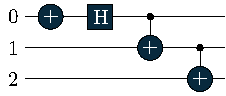
\includegraphics[width=0.3\textwidth]{src/ghz_circuit.pdf}. 
% \end{align}
% Instead of the \textsc{hadamard} we can also use a parametrized operation like $R_y(\theta)$
% \begin{align}
%     U = \textsc{cnot}(1,2)\textsc{cnot}(0,1)R_y(0,\theta)\textsc{not}(0)
% \end{align}
% the circuit representation of this operation looks basically the same. Here, we will sometimes color the parametrized gates to indicate that the parameter $\theta$ is not determined yet
% \begin{align}
%     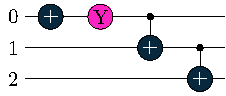
\includegraphics[width=0.3\textwidth]{src/ghz_ry_circuit.pdf}.
% \end{align}
% As a last example, we look at the circuit with the two \textsc{cnot} operations replaced by
% \begin{align}
%     R_{xy}(\theta) = e^{-i\frac{\theta}{2} X\otimes Y}  
% \end{align}
% with parametrization $\theta=\varphi$ (so a different parameter than in the $R_y$ rotation before) for the first and $\theta=\pi/2$ for the second gate. The final assembled unitary is then 
% \begin{align}
%     U = R_{xy}(\pi/2,1,2)R_{xy}(\varphi,0,1)R_y(0,\theta)\textsc{not}(0)
% \end{align}
% and the circuit is graphically depicted as
% \begin{align}
%     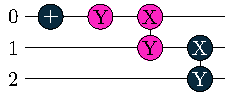
\includegraphics[width=0.3\textwidth]{src/ghz_xy_circuit.pdf},\label{eq:circuit_example_xy}
% \end{align}
% so the fact that the two parametrized gates carry individual parameters is often not emphasized (styles vary though). One can for example often see the explicit notation
% \begin{align}
%     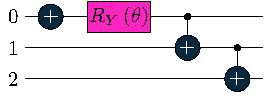
\includegraphics[width=0.3\textwidth]{src/alt_ghz_ry_circuit.pdf}.
% \end{align}

% General remarks:
% \begin{itemize}
%     \item gates that ``touch'' different qubits commute and can be executed in parallel (sometimes the collection of in-parallel executable gates is referred to as ``moments'')
%     \item runtime correlates with ``depth'' of the circuit (the number of moments in the circuit)
%     \item not all architectures are necessarily able to execute gates in parallel
% \end{itemize}
% The circuits shown so far all had depths 4 and all gates formed independent moments. Depending on what we are considering a primitive gate, these depths can however change. If only single-qubit Pauli rotations and \textsc{cnot}s are considered primitive operations, the $XY$ rotations from circuit~\eqref{eq:circuit_example_xy} need to be decomposed into sequences of those operations. In this chapter we will see how we can do this through a general framework generated by Pauli matrices.

\clearpage
\section{Pauli Formalism}
In the following we will develop a convenient formalism build from the three Pauli symbols ${\sigma_0,\sigma_1,\sigma_2,\sigma_3}$ that is sufficient to represent all operations on quantum computers. 
The primitive symbols ${\sigma_1,\sigma_2,\sigma_3}$ have a representation as $2\times 2$ Pauli matrices, while $\sigma_0$ is just the unit operation.
\begin{def*}[Pauli Matrix]
\begin{align}
        \sigma_1\equiv X = \begin{pmatrix}
        0 & 1 \\ 1 & 0
    \end{pmatrix}, \;\;        \sigma_2\equiv Y = \begin{pmatrix}
        0 & -i \\ i & 0
    \end{pmatrix},\;\;        \sigma_3\equiv Z=  \begin{pmatrix}
        1 & 0 \\ 0 & -1
    \end{pmatrix}
\end{align}
\end{def*}
Besides many other properties, the Pauli matrices are \textit{unitary} and \textit{Hermitian} (and therefore also \textit{self-inverse})~\footnote{they are also traceless, but we won't need this property here. Note that this is the reason why $\sigma_0 = 1_{2\times 2}$ is formally not a Pauli matrix. We will however be sloppy with the naming.}
\begin{theorem*}[pauli algebra]
Pauli matrices are unitary and Hermitian at the same time
\begin{align}
    \sigma_k ^\dagger = \sigma_k = \sigma_k^{-1}.\label{eq:pauli-algebra}
\end{align}
The product of two distinct Pauli matrices (not considering the unit matrix) will be proportional to the corresponding third Pauli matrix 
\begin{align}
    &XY = iZ, \;\; YX = -iZ\\
    &ZX = iY, \;\; XZ = -iY\\
    &YZ = iX, \;\; ZY = -iX
\end{align}
where the sign can be determined if the string of Paulis from left to right is an odd or even permutation from $XYZ$.
From the multiplication it follows direclty that the Pauli matrices transform anti-symmeric under themselves
\begin{align}
    \sigma_k \sigma_l \sigma_k = - \sigma_l,\; \forall k\neq l\in \left\{x,y,z\right\}.
\end{align}
\end{theorem*}
Take as explicit example (which we will also need further down)
\begin{align}
    XZX = -Z\label{eq:XZX=-Z}.
\end{align}
We can now generate operations on multiple qubits via tensor products.
\begin{def*}[Paulistring]
An $N$-qubit Paulistring is given by
    \begin{align}
        P_{\mathbf{k}} = \bigotimes_{i=1} ^{N} \sigma_{k_i}
    \end{align}
    where $\mathbf{k}=\left[k_1,k_2,k_3,\dots, k_N\right]$ and each $k_i\in \left\{0,1,2,3\right\}$
\end{def*}
It is often useful to use ``normal'' products instead of tensor products and write the qubit onto which the Pauli matrix acts in parenthesis
The two notations below are then equivalent
    \begin{align}
        P_{\mathbf{k}} = \bigotimes_{i=1} ^{N} \sigma_{k_i}=\prod_{i=1} ^{N} \sigma_{k_i}(i)
    \end{align}
and the latter has the advantage that we can drop unit matrices. Some examples
\begin{align}
    &1\otimes X \otimes Y = Y(1)X(2) \\
    &\sigma_x \otimes 1 \otimes \sigma_z = Z(1)X(3).
\end{align}
As the Pauli matrices, any Paulistring is \textit{unitary} and \textit{Hermitian}
\begin{align}
    P_\mathbf{k} ^\dagger = P_\mathbf{k} = P_\mathbf{k}^{-1}.
\end{align}

\begin{theorem*}[Pauli basis]
Any $2\times 2$ matrix can be represented as a linear combination of the four Pauli symbols.
\end{theorem*}
We can see this by representing the ``standard'' basis in terms of the Paulis
\begin{align}
    &\begin{pmatrix}
        1 & 0 \\0 & 0
    \end{pmatrix} = \ket{0}\bra{0}=  \frac{1}{2}\left(1 + Z\right),\;\;
    \begin{pmatrix}
    0 & 0 \\0 & 1
    \end{pmatrix} = \frac{1}{2}\left(1 - Z\right) = \ket{1}\bra{1}\\
    &\begin{pmatrix}
        0 & 1 \\0 & 0
    \end{pmatrix} = \ket{0}\bra{1} =  \frac{1}{2}\left(X + iY\right),\;\;    \begin{pmatrix}
        0 & 0 \\1 & 0
    \end{pmatrix}  = \ket{1}\bra{0}= \frac{1}{2}\left(X - iY\right) 
\end{align}
where the short-notation $\sigma_{\pm} = 1/2(X \pm iY)$ is fairly common.
In the same manner we have
\begin{theorem*}[Pauli basis]
Any $2^N\times 2^N$ matrix can be represented as a linear combination of all possible $N$-qubit Pauli strings.
\end{theorem*}
You can see this by thinking about the standard basis in $2^N$ dimension as the tensor product of the standard basis in $2^{N-1}$ dimensions. Just try to build the 4 basis matrices for $4\times 4$ matrices as tensor products from the $2\times 2$ standard basis matrices. Now you can use the formulas above to decompose back into Paulistrings. Here is an example
\begin{align}
    \begin{pmatrix}
        0 & 0 & 0 & 0\\
0 & 0 & 1 & 0\\
0 & 0 & 0 & 0\\
0 & 0 & 0 & 0\\
    \end{pmatrix} &= \ket{1}\bra{2} = \ket{01}\bra{10}\nonumber\\ 
    &=\ket{0}\bra{1}\otimes\ket{1}\bra{0} = \sigma_+ \otimes \sigma_- \nonumber\\
    &= \frac{1}{4}\left(X\otimes X - iX\otimes Y + i Y\otimes X + Y\otimes Y\right)
\end{align}
Representing a matrix as a linear combination of Pauli matrices has some advantages compared to the standard basis.
\begin{theorem*}
    A matrix $M$ that can be represented as a linear combination of Pauli matrices
    \begin{align*}
        M = \sum_{k} c_k P_\mathbf{k}
    \end{align*}
    is Hermitian ($M^\dagger=M)$ iff all $c_k$ are real numbers, and anti-Hermitian ($M^\dagger = - M$) iff all $c_k$ are purely imaginary.
\end{theorem*}
In a way you can think about Hermitian and anti-Hermitian matrices as the equivalent of real and imaginary parts of a matrix~\footnote{You can also write any general matrix as $M=H + A$ with Hermitian $H=\frac{1}{2}(M+M^\dagger)$ and anti-Hermitian $\frac{1}{2}(M - M^\dagger)$ similar to real and imaginary parts of a complex number. In the Paulistring representation $M=\sum_k c_k P_k$ with complex numbers $c_k = a_k + ib_k$ we have $H=\sum_k a_k P_k$ and $A=\sum_k ib_k P_k$.} Just don't get confused: A Hermitian matrix can have complex entries (see for example the Pauli $Y$ matrix) but in the Pauli representation it will only have real coefficients.\\
We can use this to define a datatype with corresponding datastructure
\begin{def*}[$N$-Qubit Hermitian Operation]\phantom{...}\\
    A set of tuples $\left\{(c_k,P_\mathbf{k})\right\}_{k=1}^N$ with $c_k\in \mathbb{R} $ and $P_k$ a Paulistring.\\

    Represents the operation
    \begin{align*}
        H = \sum_k c_k P_\mathbf{k}.
    \end{align*}
\end{def*}

\subsection{Pauli Gates}

We know now how to represent any matrix on $N$-qubits, including the for important Hermitian matrices, as a linear combination of Paulistrings.
Of course we can also represent unitary matrices as linear combination of Pauli strings, compared to the Hermitian matrices there is however no simple trick on how to ensure that the matrix is unitary. 
Rather than having a sum, it is more convenient to use products to represent unitary matrices~\footnote{Hermitians are closed under addition: if $B,D$ are Hermitian then $A = B + C$ is Hermitian while unitaries are closed under multiplication: if $B,D$ are unitary, then $A = BD$ is untary.}
If we represent a unitary $U$ as a product of other unitaries $U=U_mU_{m-1}U_{m-2}\dots U_1$ we call this a quantum circuit and the individual $U_m$ quantum gates.
The Paulistrings themselves are not the best primitives for a product representation, since a product of two Paulistrings is always another Paulistring, so we would be way to restricted to represent arbitrary unitary matrices. 
\begin{def*}[Pauli Gate]
    The Pauli gate is a unitary matrix generated by a Paulistring
    \begin{align}
        R_\mathbf{k}(\theta) = e^{-i\frac{\theta}{2} P_\mathbf{k}}
    \end{align}
    where $\theta \in \mathbf{R}$ and the $-1/2$ is a convention that we will follow for consistency with the literature.
\end{def*}
It turns out that the Pauli gate is \textit{universal}, meaning roughly that we can represent any unitary as a product of Pauli gates $R_\mathbf{k}(\theta_k)$ (with corresponding angles $\theta_k$ set to concrete values) to arbitrary accuracy (so not necessarily exact, but with controllable error).  
The meaning of this statement will become clear in the next sections.
Before we turn our attention to compiling strategies with Pauli gates as gate-sets, we will take a look at common used forms and useful properties. 
\begin{theorem*}[Pauli Gate: Closed form]
All Pauli gates can be represented as
\begin{align}
    R_\mathbf{k}(\theta) = \cos\left(\frac{\theta}{2}\right) -i \sin\left(\frac{\theta}{2}\right)P_\mathbf{k}
\end{align}
\end{theorem*}
To proof the property: check the series representation for $\exp$, $\sin$, $\cos$ and use the fact that the Paulistrings are self-inverse $P_\mathbf{k}^2=1$.
From the closed form representation another useful property follows directly.
\begin{theorem*}
Paulistrings generate themselves (up to a global phase)
\begin{align}
    P_\mathbf{k} = -i R_\mathbf{k}(\pi)
\end{align}
\end{theorem*}
At this point, it might be useful to visit the appendix~\ref{sec:qubit-rep} and re-iterate what global phases are.\\

The single qubit Pauli gates (generated by $X,Y,Z$)~\footnote{the ``gate'' generated by $1$ would just be a global phase gate, and therefore not realizable in the physical sense.} are in some sense special, as they are usually considered ``standard'' operation that any high-level language should be able to support.
\begin{def*}[Single-Qubit Rotations]
    The Pauli gates generated by $X,Y,Z$ are called qubit rotations. Their matrix form (following directly from the closed-form of Pauli gates) are
    \begin{align}
        R_x(\theta) = \begin{pmatrix}
            \cos\left(\frac{\theta}{2}\right) & -i\sin\left(\frac{\theta}{2}\right) \\ -i\sin\left(\frac{\theta}{2}\right) & \cos\left(\frac{\theta}{2}\right)
        \end{pmatrix}
    \end{align}
    \begin{align}
        R_y(\theta) = \begin{pmatrix}
            \cos\left(\frac{\theta}{2}\right) & -\sin\left(\frac{\theta}{2}\right) \\ \sin\left(\frac{\theta}{2}\right) & \cos\left(\frac{\theta}{2}\right)
        \end{pmatrix}
    \end{align}
    \begin{align}
        R_z(\theta) = \begin{pmatrix}
            e^{-i\frac{\theta}{2}} & 0 \\ 0 & e^{i\frac{\theta}{2}}
        \end{pmatrix}
    \end{align}
\end{def*}
The qubit rotations are the rotation matrices for $\mathbb
{C}^2$.~\footnote{easy to see with $R_y$ which is the rotation matrix for $\mathbb{R}^2$. Just apply the matrix to any vector and see what happens.}
The fancy term here is $\operatorname{SU}(2)$, the group of ``special unitary matrices in 2 dimensions''~\footnote{special, because the determinant is always 1. We don't need the other matrices, that would then form the group $\operatorname{U}(2)$, due to the global phase equivalency. If the determinant of a matrix $U \in \mathbb{C}^{n \times n}$ is 1, then the determinant of $\tilde{U} = e^{i\varphi} U$ is $e^{i n \varphi}$. Sometimes the global phase $e^{i\varphi}$ is called a $\operatorname{U}(1)$ transformation (as you can view  it as a one dimensional matrix). So the global phase equivalence is sometimes referred to as $\operatorname{U}(1)$ invariance. }\\

\subsection{Pauli Gate Compiling}
In the following we will derive the general formula to compile an arbitrary Pauli gate $R_\mathbf{k}$ into a sequence of gates consisting only of gates in the set $\left\{\textsc{CNOT}, R_x,R_y,R_z\right\}$.\\

Lets consider the case, when all Pauli-matrices in the Paulistring $P_\mathbf{k}$ are $Z$ or $1$ -- we denote such Pauli strings as $P_\mathbf{d}$, using $\mathbf{d}$ for the index set (as it only needs to carry the non-trivial indices where the $Z$ operations act)
\begin{align}
    P_\mathbf{d}= \prod_{k\in \mathbf{d}} Z(k).
\end{align}
In this case, all standard basis states are eigenstates of $P_\mathbf{d}$~\footnote{$P_\mathbf{d}$ is a diagonal matrix, and so is $e^{-i\frac{\theta}{2}P_\mathbf{d}}$.} with eigenvalue $\pm 1$, so the gate $U_p(\theta)$ is introducing phases $e^{\mp i \frac{\theta}{2}}$ depending on the basis state it acts on. The eigenvalue is determined on the qubits where $P_\mathbf{d}$ is non-trivial -- the qubits $k\in \mathbf{d}$. If an odd number of those qubits is in state $\ket{1}$ the eigenvalue is $-1$ otherwise it is $+1$. Consider some standard computational basis state $\ket{l} \equiv \ket{l_0\dots l_{N-1}}$ on $N$ qubits
\begin{align}
    P_\mathbf{d} \ket{l_0l_1\dots l_{N-1}} =  \prod_{k\in \mathbf{d}}(-1)^{l_k} \ket{l_0l_1\dots l_{N-1}}.
\end{align}
In the same way the gate $R_{\mathbf{d}}(\theta) = e^{-i\frac{\theta}{2}P_\mathbf{d}}$ will act as
\begin{align}
    R_{P_\mathbf{d}}(\theta) \ket{l_0\dots l_{N-1}} = e^{-i\frac{\theta}{2} \prod_{k\in \mathbf{d}}{}\left(-1\right)^{l_k}} \ket{l_0\dots l_{N-1}}
\end{align}
which will evaluate to either $e^{\mp i\frac{\theta}{2}}\ket{l_0\dots l_{N-1}}$.\\


The goal is now to decompose the gate $R_{P_z}(\theta) = e^{-i\frac{\theta}{2}P_z}$ into \textsc{cnot} and single-qubit rotation gates.
At this point, we will take advantage of the property $XZX = -Z$ (see Eq.~\eqref{eq:XZX=-Z} ) of Pauli matrices 
and use \textsc{cnot} operations to flip the phase on a single $R_z$ operation placed at a qubit of our choice.
The decomposition strategy is as follows:
\begin{algo*}[$R_\mathbf{d}$ Compiling]\phantom{...}\\
Task: compile a diagonal Pauli gate $R_\mathbf{d}$ into $\textsc{cnot}$ and single Pauli rotations:\\
\begin{enumerate}
    \item pick one $k\in \mathbf{d}$
    \item add a $\textsc{cnot}(l,k)\; \forall l \in \mathbf{d}$ with $ l\neq k$
    \item place a $R_z$ rotation on qubit $k$
    \item uncompute the effect of the \textsc{cnot} sequence by adding the same sequence again.
\end{enumerate}
\end{algo*}
Let's see an example on three qubits labelled by 0,2,4 and where we pick $k=4$ in the algorithm above
\begin{equation}
    \tikzset{
        roundmini/.style={draw, circle, fill=unia2, text=white, inner sep=0.5pt, minimum size=1.2em, font=\small}
    }
    \begin{quantikz}
        \lstick{0} & \gate[style=roundmini]{\textcolor{white}{Z}} \vqw{1} & \qw \\
        \lstick{2} & \gate[style=roundmini]{\textcolor{white}{Z}} \vqw{1} & \qw \\
        \lstick{4} & \gate[style=roundmini]{\textcolor{white}{Z}}         & \qw 
    \end{quantikz}
    =
    \begin{quantikz}
        \lstick{0} & \ctrl{2} & \qw      & \qw                       & \qw      & \ctrl{2} & \qw \\
        \lstick{2} & \qw      & \ctrl{1} & \qw                       & \ctrl{1} & \qw      & \qw \\
        \lstick{4} & \targ{} & \targ{} & \gate[style=roundmini]{\textcolor{white}{Z}} & \targ{} & \targ{} & \qw 
    \end{quantikz}
\end{equation}
% \begin{align}
%     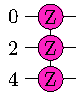
\includegraphics[height=0.1\textheight]{src/pauli_zgate_level_0.pdf}
%     \raisebox{1cm}{=}
%     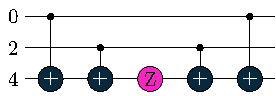
\includegraphics[height=0.1\textheight]{src/alt_pauli_zgate_level_1.pdf}.
% \end{align}
where the gates that carry the parameter $\theta$ are marked in purple.
The strategy works as well with a ``ladder'' arrangement of the \textsc{cnots}.
Take for example
\begin{equation}
    \tikzset{
        roundmini/.style={draw, circle, fill=unia2, text=white, inner sep=0.1pt, minimum size=1.2em, font=\small}
    }
    \begin{quantikz}
        \lstick{} & \gate[style=roundmini]{\textcolor{white}{Z}} \vqw{1} & \qw \\
        \lstick{} & \gate[style=roundmini]{\textcolor{white}{Z}} \vqw{1} & \qw \\
        \lstick{} & \gate[style=roundmini]{\textcolor{white}{Z}}         & \qw 
    \end{quantikz}
    =
    \begin{quantikz}
        \lstick{} & \ctrl{1} & \qw      & \qw                       & \qw      & \ctrl{1} & \qw \\
        \lstick{} & \targ{}     & \ctrl{1} & \qw                       & \ctrl{1} & \targ{}       & \qw \\
        \lstick{} & \qw & \targ{} & \gate[style=roundmini]{\textcolor{white}{Z}} & \targ{} & \qw & \qw 
    \end{quantikz}.
\end{equation}
% \begin{align}
%     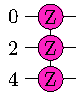
\includegraphics[height=0.1\textheight]{src/pauli_zgate_level_0.pdf}
%     \raisebox{1cm}{=}
%     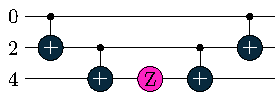
\includegraphics[height=0.1\textheight]{src/pauli_zgate_level_1.pdf}.
% \end{align}


Finally it is just a small step from the ``all-Z'' (or a  $R_\mathbf{k}$) generator to a general Pauli gate $R_\mathbf{k}$.
We essentially just have to come up with a small circuit that diagonalized $R_\mathbf{k}$ which is the same circuit that diagonalized the Pauli string $P_\mathbf{k}$ itself -- but let's clarify this first.
Assume you have a unitary that diagonalized $P_\mathbf{k}$, let's call it $U_\mathbf{k}$ since it will obviously depend on $\mathbf{k}$
\begin{align}
    U_\mathbf{k} P_\mathbf{k}U_\mathbf{k}^\dagger = P_\mathbf{d}
\end{align}
then this unitary also diagonalized $R_\mathbf{k}$ which can can easily see over the closed-form of the gate~\footnote{this relation however also holds if no closed form is available, just via the exponential series and the following trick (here shown for exponent 3): $P_\mathbf{k}^3 = P_\mathbf{k}P_\mathbf{k}P_\mathbf{k} = P_\mathbf{k}1P_\mathbf{k}1P_\mathbf{k} = P_\mathbf{k}U_\mathbf{k}^\dagger U_\mathbf{k} P_\mathbf{k}U_\mathbf{k}^\dagger U_\mathbf{k}P_\mathbf{k} $.}
\begin{align}
    U_\mathbf{k}R_\mathbf{k}(\theta)U_\mathbf{k}^\dagger &= \cos(\theta/2) -i \sin(\theta_2)U_\mathbf{k}P_\mathbf{k}U_\mathbf{k}^\dagger  \nonumber\\
    &= \cos(\theta/2) -i \sin(\theta_2)P_\mathbf{d}\nonumber\\
    &= e^{-i \frac{\theta}{2}P_\mathbf{d}} = R_\mathbf{d}(\theta).
\end{align}

All that's left is now to construct the diagonalizing unitary $U_\mathbf{k}$. 
Since $P_\mathbf{k}$ is just a product of Pauli matrices, the unitary $U_\mathbf{k}$ can just individually diagonalize them, so the unitary will also have a product structure
\begin{align}
    U_\mathbf{k} = \prod_{i=1}^N U_{k_i}(i)
\end{align}
and the $U_{k_i}$ will diagonalize the Pauli matrix $\sigma_{k_i}$. For unit matrix $k_i=0$ and $Z$ ($k_i=3$) there is nothing to do, which leaves us only with the $X$ and $Y$ cases.\footnote{Note that we already know a operation that diagonalized $X$ which is the Hadamard operation, but we are now trying to find a single qubit Pauli gate that does the job.}
By playing with the closed-form of Pauli gates and the Pauli algebra anti-symmetric transformation properties, we find soon that $R_y$ is a good candidate to diagonalize $X$ and vice versa. 
We give the details for the $X$ case:
\begin{align}
    R_y(-\pi/2) X R_y(-\pi/2)^\dagger &= R_y(-\pi/2) X R_y(\pi/2) \nonumber\\
    &= \left(\cos(\pi/4) + i\sin(\pi/4)Y  \right) X \left(\cos(\pi/4) - i\sin(\pi/4)Y  \right) \nonumber\\
    &= \frac{1}{{2}}\left(1 + iY \right) X \left(1 - i Y \right) \nonumber\\
    &= \frac{1}{2}\left(X -iXY + iYX + YXY\right) = \frac{1}{2}\left(X -2iXY - X\right)\nonumber\\
    &= -iXY = -i(iZ) = Z
 \end{align}
 where we repeately used the properties of the Pauli algebra (see Eq.~\eqref{eq:pauli-algebra} and following).
 \begin{algo*}[Pauli Basis Change]
     We can use $R_y(-\pi/2)$ and $R_x(\pi/2)$ to switch from $Y$ and $X$ to $Z$ and back
     \begin{align}
         &R_y(-\pi/2) X R_y(-\pi/2)^\dagger = Z
    \end{align}
    \begin{align}
         &R_x(\pi/2) Y R_x(\pi/2)^\dagger = Z
     \end{align}
    Any Pauli-Gate $R_\mathbf{k}$ can then be transformed into a diagonal Pauli gate $R_\mathbf{d}$ with the circuit
    \begin{align}
        U_\mathbf{k} = \prod_{i=1}^N U_{k_i}
    \end{align}
    with
    \begin{align}
        U_{k_i} = \begin{cases}
            R_x(\pi/2), & k_i = Y\\
            R_y(-\pi/2), & k_i = X\\
            1, & \text{else}
        \end{cases}\;\;.
    \end{align}
 \end{algo*}
To conclude the compilation of Pauli gates: for a general Paulistring we initially transform all non-diagonal Paulis (i.e. $X$ and $Y$) into $Z$, and then compile with 


\begin{equation}
\begin{quantikz}
    \lstick{0} & \gate[style={draw, circle, inner sep=0.1pt, fill=unia2, text=white}]{\textcolor{white}{X}} \vqw{1} & \qw \\
    \lstick{2} & \gate[style={draw, circle, inner sep=0.1pt, fill=unia2, text=white}]{\textcolor{white}{Y}} \vqw{1} & \qw \\
    \lstick{4} & \gate[style={draw, circle, inner sep=0.1pt, fill=unia2, text=white}]{\textcolor{white}{Z}} & \qw 
\end{quantikz}
=
\begin{quantikz}
    \lstick{0} & \gate[style={draw, circle, fill=fai, inner sep=0.01pt}]{Y_+} & \ctrl{1} & \qw      & \qw                                           & \qw      & \ctrl{1} & \gate[style={draw, circle, fill=fai, inner sep=0.1pt}]{Y_-} & \qw \\
    \lstick{2} & \gate[style={draw, circle, fill=fai,inner sep=0.01pt}]{ X_+} & \targ{}  & \ctrl{1} & \qw                                           & \ctrl{1} & \targ{}  & \gate[style={draw, circle, fill=fai, inner sep=0.01pt}]{X_+} & \qw \\
    \lstick{4} & \qw                                           & \qw      & \targ{}  & \gate[style={draw, circle,  inner sep=0.01pt, fill=unia2}]{\textcolor{white}{Z}} & \targ{}  & \qw      & \qw                                           & \qw 
\end{quantikz}
\end{equation}
We used the short notation $X_\pm = R_x(\pm \pi/2)$ for the basis changes with $X_+^\dagger = X_-$.
\begin{algo*}[$R_\mathbf{k}$ Compiling]
Task: Compile a general Pauli gate $R_\mathbf{k}$ into \textsc{cnot} and single Pauli rotations. The color code (here in purple) indicates which gates are carrying the angle $\theta$.
\begin{enumerate}
    \item Assemble a diagonalizing unitary $U_\mathbf{k}$ (Pauli Basis Change)
    \item Assemble a circuit $U_c$ that implements $R_\mathbf{d}$ where all non-diagonal entries in $P_\mathbf{k}$ are treated as $Z$
    \item result: $U_\mathbf{k}^\dagger U_c U_\mathbf{k}$
\end{enumerate}
\end{algo*}

We now know how to compile every Pauli gate $R_\mathbf{k}$ into a sequence of gates in the set 
\begin{align}
    \left\{R_x,R_y,R_z, \textsc{cnot}\right\}.
\end{align}
We need $R_x$ and $R_y$ for the basis change from $P_\mathbf{k}$ to a diagonal $P_\mathbf{d}$ and the $\textsc{cnot}$ and $R_z$ to compile $R_\mathbf{d}$ further.
We can use the same strategy to compile into
\begin{align}
     \left\{\hd, R_x,R_z, \textsc{cnot}\right\} 
\end{align}
since the Hadamard gate also does the job of diagonalizing $X$.
With the same reasoning we could also compile to
\begin{align}
     \left\{\hd, S ,R_z, \textsc{cnot}\right\} 
\end{align}
where the $S$ gate is
\begin{align}
    S = \begin{pmatrix}
        1 & 0 \\ 0 & i
    \end{pmatrix}\;,
\end{align}
and we can build a circuit that diagonalizes $Y$ from $\hd$ and $S$ (try yourself). Since $S = T^2$ the set
\begin{align}
     \left\{\hd, T ,R_z, \textsc{cnot}\right\} 
\end{align}
works as well.
If we remember the global phase equivalency (see appendix) we can also work our way through an implementation of $T$ (or $S=T^2$) with the $R_z$ gate
\begin{align}
    R_z(\pi/4) = e^{-i\frac{\pi}{8}} T.
\end{align}
meaning that the set 
\begin{align}
     \left\{\hd, R_z, \textsc{cnot}\right\}\label{eq:H,Rz,cnot} 
\end{align}
already suffices.
In the following section we will see that Pauli gates are universal. Since we can compile Pauli gates into any of the sets above, all of them are universal as well.

\subsection{Compiling to Pauli Gates}
Multi qubit gates (operations on multiple qubits) can always be representable as
\begin{align}
    U = e^{-i\frac{\theta}{2} G}
\end{align}
with a suitable Hermitian generator $G$ that itself can always be represented as linear combination of Paulistrings (see Pauli representation above). Problem: Paulistrings don't commute~\footnote{The commutator of two matrices $A,B$ is defined as $[A,B]=AB-BA$. Paulis don't necessarily commpute: e.g. $[X,Y] = XY - YX = XY - (-XY) = 2XY = 2iZ$ (see Pauli algebra from the previous section)} so we can't just use the usual formulas for exponentials in order to get this in a product form. Fortunately, non-commuting mathematical structures have been studied in many forms. One result that comes in Handy is the Lie formula.
\begin{theorem*}[Lie Formula]
    For two square matrices $A,B$ we have
\begin{align}
    e^{A+B} = \lim_{n \rightarrow \infty } \left(e^{A/n}e^{B/n}\right)^n,
\end{align}
or for quantum operations 
\begin{align}
    e^{-i\frac{\theta}{2}\left(A+B\right)} = \lim_{n \rightarrow \infty } \left(e^{-i\frac{\theta}{2n}A}e^{-i\frac{\theta}{2n} B
    }\right)^n.
\end{align}
\end{theorem*}
Proof sketch: First realize that the non-commutativity of $A$ and $B$ plays no role up to linear order
\begin{align}
    e^{-i\frac{\theta}{2} \left(A + B\right)} = 1 - i\frac{\theta}{2} A - i\frac{\theta}{2} B + \dots \\
    e^{-i\frac{\theta}{2} \left(A\right)}e^{-i\frac{\theta}{2} \left(B\right)} = 1 - i\frac{\theta}{2} A - i\frac{\theta}{2} B + \dots. 
\end{align}
For ``sufficiently small'' angles $\theta$ linear order is good enough. The idea is now to take $n$ small steps, \textit{i.e.} to take $n$ small rotations $\theta/n$, instead of one large step
\begin{align}
    e^{-i\frac{\theta}{2}\left(A+B\right)} \approx \left(e^{-i\frac{\theta}{2n}A}e^{-i\frac{\theta}{2n} B
    }\right)^n
\end{align}
In the limit $n \rightarrow \infty$ this approximation becomes exact. We can generalize this result to arbitrary generators constructed as sums of primitive elements -- here we take the Paulistrings.
\begin{theorem*}[Trotter Decomposition]
A general unitary $e^{-i\frac{\theta}{2}G}$ represented through a generator $G=\sum_k c_k P_\mathbf{k}$ assembled from Paulistrings can be decomposed as
\begin{align}
    U = e^{-i\frac{\theta}{2} 
    \sum_k\left( c_k P_\mathbf{k} \right)} = \lim_{n\rightarrow\infty} \left(\prod_{k} e^{-i\frac{\theta_k}{2n} P_\mathbf{k}} \right)^n= \lim_{n\rightarrow\infty} \left( \prod_k R_\mathbf{k}\left({\frac{\theta_k}{n}}\right)\right)^n\label{eq:trotter}
\end{align}  
with $\theta_k = c_k\cdot \theta$.
\end{theorem*}
There are ways to control the Trotter error, but in practice one often takes a finite $n$ and hopes its suitable for the task at hand. With Eq.~\eqref{eq:trotter} in combination with the Pauli compiling scheme from the previous section, we can now decompose any multi-qubit gate into \textsc{cnot} and single-pauli rotations, as long as we know it's generator.

Remarks on the Trotter decomposition in Eq~\eqref{eq:trotter}
\begin{itemize}
    \item There is no canonical ordering
    \item Estimating errors is not easy
    \item Higher-order formulas exist
\end{itemize}

\subsection{Controlled Gates}
For any given unitary $U$ we can formally construct a controlled-version $CU$. If $U$ is an $N$-qubit unitary, then $CU$ is a $N+1$ qubits unitary that acts as
\begin{align}
    CU\left(\ket{\Psi}\otimes\ket{k}\right) = \begin{cases}
        U\ket{\Psi}\otimes \ket{k}, & k=1 \\
        \left(\ket{\Psi}\otimes\ket{k}\right), & \text{else}
    \end{cases}
\end{align}
meaning, the control qubit acts as a  switch for the operation on the remaining $N$ qubits. Graphically the control element is symbolized by a bold dot on the circuit and the most prominent controlled operation, which we already encountered many times, is the controlled-not.\\
\begin{theorem*}
If we know the matrix representation of $U$, then the matrix that represents $CU$ is
\begin{align}
   CU =  \begin{pmatrix}
        \textbf{1} & \textbf{0} \\
        \textbf{0} & \textbf{U}
    \end{pmatrix}.
\end{align}
\end{theorem*}
This is not very helpful for circuit decompositions, but can come in handy for general analysis.\\

\begin{algo*}[Control-Compiling]
  If we know the generator for our unitary operation of interest, meaning we can write
\begin{align}
    U = e^{-i\frac{\theta}{2} G}
\end{align}
with $G$ Hermitian, then the controlled version of this unitary is
\begin{align}
    CU = e^{-i\frac{\theta}{2} \ket{1}\bra{1}\otimes G} = e^{-i\frac{\theta}{2} 
\frac{1}{2}\left(1-Z\right)\otimes G}\label{eq:controlled-generator}.
\end{align}  
\end{algo*}
Note that this works for all generators $G$, not just single-qubit operations. 
If the unitary is a simple Pauli gate $R_\mathbf{k}$, then it suffices to only put the control on the $R_z$ after the compilation of the Pauli gate (as the basis change and \textsc{cnot} ladders will all cancel each other, if the central $R_z$ is switched off).
With this motivation in mind:
Let's try the controlled-$R_z$ rotation as an example
\begin{align}
    CR_z\left(\theta\right) = e^{-i\frac{\theta}{2}\frac{1}{2} \left(1-Z\right)Z} = e^{-i\frac{\theta}{4} Z\otimes Z}e^{+i\frac{\theta}{4} 1\otimes Z},
\end{align}
or in graphical language
% \begin{align}
% 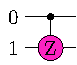
\includegraphics[height=0.1\textwidth]{src/crz_0.pdf}\raisebox{0.6cm}{=}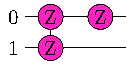
\includegraphics[height=0.1\textwidth]{src/alt_crz_1.pdf}\raisebox{0.6cm}{=}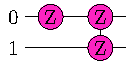
\includegraphics[height=0.1\textwidth]{src/alt2_crz_1.pdf}.
% \end{align}

\begin{equation}
    \tikzset{
        roundmini/.style={draw, circle, fill=unia2, text=white, inner sep=0.1pt, minimum size=1.2em, font=\small}
    }
    \begin{quantikz}
        \lstick{} & \ctrl{1} & \qw \\
        \lstick{} & \gate[style=roundmini]{\textcolor{white}{Z}} & \qw 
    \end{quantikz}
    =
    \begin{quantikz}
        \lstick{} & \gate[style=roundmini]{\textcolor{white}{Z}} \vqw{1} & \gate[style=roundmini]{\textcolor{white}{Z}} & \qw \\
        \lstick{} & \gate[style=roundmini]{\textcolor{white}{Z}}         & \qw                       & \qw 
    \end{quantikz}
    =
    \begin{quantikz}
        \lstick{} & \gate[style=roundmini]{\textcolor{white}{Z}} & \gate[style=roundmini]{\textcolor{white}{Z}} \vqw{1} & \qw \\
        \lstick{} & \qw                       & \gate[style=roundmini]{\textcolor{white}{Z}}         & \qw 
    \end{quantikz}
\end{equation}
where we lose the information about the angle (going from $\theta$ to $\theta/2$).
We can move the individual $R_z$ on the first qubit freely through the $R_{ZZ}$ gate on both qubits, since the $Z$ generator commutes with the $Z\otimes Z$ generator.\\
If we now apply the Pauli compiling scheme from before to the $R_{ZZ}$ gate, we get
\begin{equation}
    \tikzset{
        roundmini/.style={draw, circle, fill=unia2, text=white, inner sep=0.1pt, minimum size=1.2em, font=\small}
    }
    \begin{quantikz}
        \lstick{} & \gate[style=roundmini]{\textcolor{white}{Z}} & \gate[style=roundmini]{\textcolor{white}{Z}} \vqw{1} & \qw \\
        \lstick{} & \qw                       & \gate[style=roundmini]{\textcolor{white}{Z}}         & \qw 
    \end{quantikz}
= 
    \begin{quantikz}
        \lstick{} & \gate[style=roundmini]{\textcolor{white}{Z}} & \ctrl{1} & \qw & \ctrl{1} & \qw \\
        \lstick{} & \qw                       & \targ{} & \gate[style=roundmini]{\textcolor{white}{Z}}  & \targ{}         & \qw 
    \end{quantikz}
\end{equation}
% \begin{align}
% 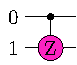
\includegraphics[height=0.1\textwidth]{src/crz_0.pdf}\raisebox{0.6cm}{=}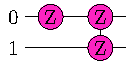
\includegraphics[height=0.1\textwidth]{src/alt2_crz_1.pdf}\raisebox{0.6cm}{=}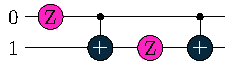
\includegraphics[height=0.1\textwidth]{src/alt3_crz_1.pdf}.
% \end{align}
Note that the $R_z$ on the first qubit can again be placed anywhere (since it's generator $Z$  commutes with the ``generator'' $\ket{1}\bra{1} = 1/2(1-Z)$ of the control in the \texttt{cnot}), so we have found a quite effective decomposition
\begin{equation}
    \tikzset{
        roundmini/.style={draw, circle, fill=unia2, text=white, inner sep=0.1pt, minimum size=1.2em, font=\small}
    }
    \begin{quantikz}
        \lstick{} & \ctrl{1} & \qw \\
        \lstick{} & \gate[style=roundmini]{\textcolor{white}{Z}} & \qw 
    \end{quantikz}
    =
= 
    \begin{quantikz}
        \lstick{} &  \ctrl{1} & \gate[style=roundmini]{\textcolor{white}{Z}} & \ctrl{1} & \qw \\
        \lstick{} &                       \targ{} & \gate[style=roundmini]{\textcolor{white}{Z}}  & \targ{}         & \qw 
    \end{quantikz}
\end{equation}
% \begin{align}
% 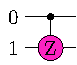
\includegraphics[height=0.1\textwidth]{src/crz_0.pdf}\raisebox{0.6cm}{=}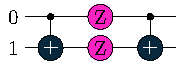
\includegraphics[height=0.1\textwidth]{src/alt4_crz_1.pdf}.
% \end{align}
Note that if the original angle was $CR_z(\theta)$, then the two parametrized gates are $R_z(\theta/2)$ (for the gate on the first qubits) and $R_z(-\theta/2)$ (for the gate on the second) -- so two different angles, not visible in the graphical representation.\\

What works with a single control also works with multiple control qubits.
\begin{algo*}[Multi-Control-Compilation] Take an $N$-qubit unitary
\begin{align}
    U = e^{-i\frac{\theta}{2} G}
\end{align}
acting on qubits $\left\{t_1,t_2,\dots,t_N\right\}$, then the controlled version with $M$ control qubits $\left\{c_1,c_2,\dots c_M\right\}$, is generated by 
\begin{align}
    \mathcal{G} = \prod_{k=1}^{M}\frac{1}{2}\left( 1-Z(q_k) \right) G(t_1,t_2,\dots,t_N).
\end{align}
\end{algo*}
As an example we take the Toffoli gate (the \textsc{ccnot}) and show the decomposition in graphical form.
We start with the generator for \textsc{not} which is $G=(X-1)$ and the gate itself is $X=e^{-i\frac{\pi}{2}(X-1)}$. The generator for Toffoli is therefore $-\frac{1}{4}\left(1-Z\right)\otimes\left(1-Z\right)\otimes\left(1-X\right) = -\frac{1}{4}\left(1-Z(1)-Z(2)-X(3)+Z(1)X(3)+Z(2)X(3)+Z(1)Z(2)-Z(1)Z(2)X(3)\right)$. Using a Hadamard operation on qubit 3 we diagonalize the $X(3)$ part of the generator and end up with
\[\frac{1}{4}\left(-1+Z(1)+Z(2)+Z(3)-Z(1)Z(3)-Z(2)Z(3)-Z(1)Z(2)+Z(1)Z(2)Z(3)\right).\] 
In the compilation of the gate we can then neglect the globale phase $e^{i\frac{\pi}{2}\frac{1}{4}}$ generated by the $1$ part of the generator~\footnote{note that you can only neglect the global phase in the final compilation, you can not neglect it, if you for example are building a controlled-Toffoli -- same as we could not neglect it here for the not gate.} and end up with a circuit of Pauli gates
\begin{equation}
    \tikzset{
        roundmini/.style={draw, circle, fill=white, text=white, inner sep=0.1pt, font=\small},
        squaremini/.style={draw, fill=white, text=white, inner sep=0.1pt, font=\small}
    }
    \begin{quantikz}
        \lstick{} & \ctrl{1} & \qw \\
        \lstick{} & \ctrl{1} & \qw \\
        \lstick{} & \targ{} & \qw 
    \end{quantikz}
    =
    \begin{quantikz}
        \lstick{} & \qw & \gate[style=roundmini]{Z} & \gate[style=roundmini]{Z} \vqw{1} & \gate[style=roundmini]{Z} \vqw{1} & \gate[style=roundmini]{Z} \vqw{2} & \qw & \qw & \qw \\
        \lstick{} & \qw & \gate[style=roundmini]{Z} & \gate[style=roundmini]{Z}         & \gate[style=roundmini]{Z}         & \qw                               & \gate[style=roundmini]{Z} \vqw{1} & \qw & \qw \\
        \lstick{} & \gate[style=squaremini]{H} & \gate[style=roundmini]{Z} & \qw & \gate[style=roundmini]{Z} & \gate[style=roundmini]{Z} & \gate[style=roundmini]{Z} & \gate[style=squaremini]{H} & \qw
    \end{quantikz}
\end{equation}
% \begin{align}
% 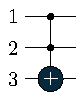
\includegraphics[height=0.15\textwidth]{src/toffoli.pdf}
% &\raisebox{1cm}{\;=\;}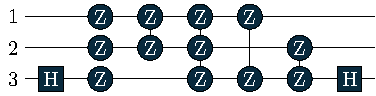
\includegraphics[height=0.15\textwidth]{src/toffoli_trotter.pdf} \nonumber\\
% \end{align}
which we can further decompose by the Pauli gate compiling scheme
% \begin{align*}
% \raisebox{1cm}{\;=\;}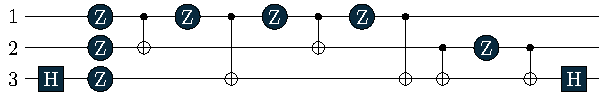
\includegraphics[height=0.1\textwidth]{src/toffoli_trotter_3.pdf} \nonumber\\
% \end{align*}
\begin{equation}
    \tikzset{
        roundmini/.style={draw, circle, fill=white, text=white, inner sep=0.1pt, font=\small},
        squaremini/.style={draw, fill=white, text=white, inner sep=0.1pt, font=\small},
    }
    \begin{quantikz}
        \lstick{1} & \qw & \gate[style=roundmini]{Z} & \ctrl{1} & \gate[style=roundmini]{Z} & \ctrl{2} & \gate[style=roundmini]{Z} & \ctrl{1} & \gate[style=roundmini]{Z} & \ctrl{2} & \qw      & \qw                       & \qw      & \qw \\
        \lstick{2} & \qw & \gate[style=roundmini]{Z} & \targ{}  & \qw                       & \qw      & \qw                       & \targ{}  & \qw                       & \qw      & \ctrl{1} & \gate[style=roundmini]{Z} & \ctrl{1} & \qw \\
        \lstick{3} & \gate[style=squaremini]{H} & \gate[style=roundmini]{Z} & \qw      & \qw                       & \targ{}  & \qw                       & \qw      & \qw                       & \targ{}  & \targ{}  & \qw                       & \targ{}  & \gate[style=squaremini]{H}
    \end{quantikz}
\end{equation}
and we have eliminated two pair of \textsc{cnot} gates on the way (as they are self inverse).


\subsection{Example: Oracle Construction (Part II)}
We will use the Pauli formalism to construct the quantum oracle used in the \texttt{Deutsch-Josza} algorithm
\begin{align*}
    U_f \ket{\mathbf{x}} = (-1)^{f(\mathbf{x})}\ket{\mathbf{x}}
\end{align*}
defined for standard basis states $\ket{\mathbf{x}}$ on $N$ qubits. 
We first note that we can also write 
\begin{align*}
    U_f \ket{\mathbf{x}} = e^{-\pi f(\mathbf{x})}\ket{\mathbf{x}},
\end{align*}
which opens up the path for generator based construction.
\begin{enumerate}
    \item Construct the Boolean function $f(\mathbf{x})$ as Hermitian generator $H\ket{\mathbf{x}}$
    \item Construct the Oracle as $U_f = e^{-i\pi H}$
\end{enumerate}
\subsubsection*{Construction of the generator}
We will use a Boolean formula in conjunctive normal form. Here, the formula consists of $M$ clauses $C_k$ connected through conjuctions (``and'' operations). Each clause contains literals (variables or negated variables) $u_i$ connected by disjunctions (``or'' operations). 
\begin{align*}
    f(\mathbf{x}) = \bigwedge_{k=1}^{M} \bigvee_{u\in C_k} u
\end{align*}
typical variants are $3$-SAT (each clause only has 3 literals at most) that look for example like
\begin{align*}
    f(\mathbf{x}) = \left(x_1 \vee x_2 \vee x_3\right) \wedge \left(\bar{x}_1 \vee x_4 \vee \bar{x}_8\right) \wedge \dots .
\end{align*}
Take for example a formula with 3 variables consisting of a single clause with 3 literals
\begin{align*}
    f(x_1,x_2,x_3) = x_1 \vee \bar{x}_2 \vee x_3
\end{align*}
the formula is always true, except for the assignment $x_1=0, x_2=1, x_3=0$. The generator 
\begin{align}
    H &= \ket{010}\bra{010} = \frac{1}{2^3}\left(1+Z(1)\right)\left(1-Z(2)\right)\left(1+Z(3)\right)\nonumber\\
    &= \frac{1}{8}\left(1+Z_1-Z_2+Z_3-Z_1Z_2+Z_1Z_3 - Z_2Z_3 - Z_1Z_2Z_3\right).
\end{align}
This generator has the same behaviour: eigenvalue 0 for basis state $\ket{010}$ and eigenvalue $+1$ for all other basis states.
In general the rule to construct a generator from a single clause is can be set to
\begin{align}
    \bigvee_{u\in C}^{} u \rightarrow H_C = \bigotimes_{k=1}^N p_k
\end{align}
with 
\begin{align}
    p_k = \begin{cases}
        \ket{0}\bra{0}, & x_k \in C\\
        \ket{1}\bra{1}, & \bar{x}_k \in C\\
        1, & \text{else}
    \end{cases}
\end{align}
where $x_k\in C$ is true, if the variable $x_i$ appears as literal in the clause. Note that we assume that trivial cases like $(x_k \in C) \wedge (\bar{x}_k\in C)$ have been removed from the clause.
For a general formula in conjunctive normal form, we can now construct a generator for each clause and multiply them together 
\begin{align*}
    f(\mathbf{x}) = \bigwedge_{k=1}^{M} \bigvee_{u\in C_k} u \rightarrow H_f = \prod_{k=1}^{M} H_{C_M}.
\end{align*}
This works, because our operator is diagonal (and therefore consists only of $1$ and $Z$ operations -- the products stay Hermitian (note that this is not in general the case).
\subsubsection*{Constructing the Oracle}
To construct the oracle as $U_f = e^{-\pi H_f}$ we don't need a Trotter decomposition (the generator is diagonal) and also no basis change (same reason). 
We will use the same example as in the previous chapter and just use the simple formula
\begin{align}
    f(\mathbf{x}) = (x_1\vee x_2\vee \bar{x}_3).
\end{align}
The generator is
\begin{align}
    H_f = \frac{1}{8}\left(1 + Z_1 + Z_2 - Z_3 + Z_1Z_2 + Z_1Z_3 - Z_2Z_3 - Z_1Z_2Z_3\right)
\end{align}
and the corresponding circuit is 
\begin{center} 
\tikzset{
        roundmini/.style={draw, circle, fill=unia2, inner sep=0pt, font=\small}
    }
\resizebox{\textwidth}{!}{%
\begin{quantikz}[column sep=0.7em, row sep=0.7em]
\lstick{$\ket{x_1}$} & \gate[style=roundmini]{\textcolor{white}{z}}       & \ctrl{1} & \qw  & \ctrl{1} & \ctrl{2} & \qw  & \ctrl{2} & \qw      & \qw  & \qw      & \ctrl{1} & \qw      & \qw  & \qw      & \ctrl{1} & \qw \\
\lstick{$\ket{x_2}$} & \gate[style=roundmini]{\textcolor{white}{z}}       & \targ{}  & \gate[style=roundmini]{\textcolor{white}{z}}  & \targ{}  & \qw      & \qw  & \qw      & \ctrl{1} & \qw  & \ctrl{1} & \targ{}  & \ctrl{1} & \qw  & \ctrl{1} & \targ{}  & \qw \\
\lstick{$\ket{x_3}$} & \gate[style=roundmini]{\textcolor{white}{z}}      & \qw      & \qw  & \qw      & \targ{}  & \gate[style=roundmini]{\textcolor{white}{z}}  & \targ{}  & \targ{}  & \gate[style=roundmini]{\textcolor{white}{z}}  & \targ{}  & \qw      & \targ{}  & \gate[style=roundmini]{\textcolor{white}{z}}  & \targ{}  & \qw      & \qw
\end{quantikz}%
}
\end{center}

Compared to the old construction (lets call this the direct construction), this seems way simpler (but less straightforward on first glance).~\footnote{Exercise: The circuit currently reflexts the order by which the individual parts of the generator where denotes in the equation above. Since all parts commute the order does not matter here. By changing the order of the individual parts of the generator, you can save up to four \texttt{cnot} operations.} Notable differences
\begin{itemize}
    \item Direct construction needs auxiliary helper qubits
    \item Direct construction results in a deeper circuit~\footnote{the decomposition of the triple and double controlled nots will take its toll}
    \item Direct construction does not need parametrized gates, like the $R_z(\pm \pi/4)$ gates used here but uses only classical logic gates (except for that two Hadamards). This can become a technical issue, when multiple clauses are involved and the angles become smaller and smaller through multiplication operations. 
\end{itemize}

To avoid the issue of exponentially vanishing angles, we could resort to a hybrid strategy: encode each clause with the Pauli formalism, saving in circuit depth by avoiding direct construction through multi-controlled not operations, but chosing the operation such that the result of a single clause is stored on one additional qubit. In the end we have at most as many additional qubits as clauses, these can then be checked with and gates (Toffoli operations). 
For this to work we would need an operation
\begin{align}
    U\left(\ket{0}\otimes\ket{\mathbf{x}}\right) =  \ket{C(\mathbf{x})}\otimes\ket{\mathbf{x}}
\end{align}
where a single qubit in the first register suffices, since for a single clause $C(\mathbf{x})\in \left\{0,1\right\}$.
The Quantum Phase Estimation (\texttt{QPE}) is an algorithm that does the job.



\clearpage
\section{Quantum Phase Estimation}
One of the most important quantum algorithms to date is the quantum phase estimation \texttt{QPE}.
It allows to measure the eigenvalues of unitary matrices
\begin{align}
    U \ket{\alpha} = e^{i\alpha} \ket{\alpha}, \;\; \alpha \in \mathbb{R}
\end{align}
and by extension also the eigenvalues of Hermitian matrices
\begin{align}
       H \ket{\alpha} = \alpha \ket{\alpha}, \;\; \alpha \in \mathbb{R} 
\end{align}
through the exponential connection $U=e^{iH}$.~\footnote{In a way the \texttt{QPE} gives an explicit implementation of the quantum mechanical axiom that observables are described through Hermitian matrices, with their eigenvalues being the observable quantities.}

As we want to use qubits to ``read-out'' our eigenvalues $\alpha$ we need to make some approximations as real numbers can not be exactly described by a finite sequence of bits.
For now we will operate under assumption that $\alpha = 2\pi \frac{k}{2^n}$ with integers $n \in \mathbb{N}$ and $0 \leq k < 2^n$, meaning that we assume our eigenvalues can be exactly represented with $n$ bits where $k$ is an integer represented by the bitstring $\mathbf{k}$.

\begin{algo*}[\texttt{QPE}: High-Level Description]\phantom{...}\\
Given a Hermitian $H$ with eigenstates $\ket{\alpha}$, eigenvalues $\alpha = 2\pi \frac{k}{2^n}$, and $k$ being a integer represented by bitstring $\mathbf{k}$, then
\texttt{QPE} will act on eigenstates $\ket{\alpha}$ as
\begin{align}
    \texttt{QPE} \left(\ket{\mathbf{0}} \otimes \ket{\alpha}\right) = \ket{\mathbf{k}} \otimes \ket{\alpha}.
\end{align}
\end{algo*}
The \texttt{QPE} operates on two qubit registers: one representing the state of interest $\ket{\alpha}$ (the state register) and another auxilliary $n$-qubits (the read-out register).

Measurement of the first qubit register now gives back the information about the phase $\alpha = 2\pi \frac{k}{2^n}$ by providing $k$ in binary. Note that the eigenstate in the second register remains unchanged -- in fact, the form $\ket{\psi} \otimes \ket{\alpha}$, with $\ket{\psi}$ being some state on the first register, remains intact throughout the whole algorithm.

In the following we are gonna approach the \texttt{QPE} in a step-by-step approach figuring out how to construct it.

\subsection{Single Qubit Case}
In the case that $n=1$, the \texttt{QPE} can be implemented as 
\begin{align}
    \texttt{QPE} = H(q_1) CU(q_1,q_2) H(q_1) 
\end{align}
or as circuit diagram (also indicating where to read-out after the unitaries are executed):
\begin{center}
$ \texttt{QPE}$ = \begin{quantikz}
& \gate{H} & \ctrl{1}& \gate{H} & \meter{} & \\
& \hphantomgate{} & \gate{U} &  \hphantomgate{} &\qw  
\end{quantikz}
\end{center}
Let's see what this circuit computes when applied to an eigenstate of $U$
\begin{align}
    \texttt{QPE}\left(\ket{0}\otimes\ket{\alpha}\right) &= \frac{1}{\sqrt{2}} H(q_1) \left( CU(q_1,q_2) \ket{0}\otimes\ket{\alpha} + CU(q_1,q_2)\ket{1}\otimes\ket{\alpha}\right) \\
    &= \frac{1}{\sqrt{2}} H(q_1) \left( \ket{0}\otimes\ket{\alpha} + e^{i\alpha}\ket{1}\otimes\ket{\alpha}\right) \\
    &= \frac{1}{\sqrt{2}} H(q_1) \left( \ket{0} + e^{2\pi i \frac{k}{2} }\ket{1}\right)\otimes\ket{\alpha}\\
    &= \frac{1}{\sqrt{2}} \left( \ket{+} + e^{2\pi i \frac{k}{2} }\ket{-}\right)\otimes\ket{\alpha}\label{eq:qpe-1qubit}
\end{align}
now remember that by our initial assumption, we are only considering matrices $U$ with eigenvalues exactly representable as $\alpha = 2\pi k/2^n$ -- so for $n=1$ we have two possibilities $k=0$ and $k=1$
\begin{align}
    \texttt{QPE}\left(\ket{0}\otimes\ket{\alpha}\right) &= \frac{1}{\sqrt{2}} 
    \begin{cases}
    \ket{+} + \ket{-} \otimes \ket{\alpha} \text{ for } k=0 \\
    \ket{+} - \ket{-} \otimes \ket{\alpha} \text{ for } k=1
    \end{cases}
\end{align}
Since we have $1/\sqrt{2}(\ket{+}+\ket{-}) = \ket{0}$ and $1/\sqrt{2}(\ket{+}-\ket{-}) = \ket{1}$, we can summarize as
\begin{align}
   \texttt{QPE}\left(\ket{0}\otimes\ket{\alpha}\right) & = \ket{k}\otimes\ket{\alpha}
\end{align}
so this is exactly what \texttt{QPE} promised to do.

\subsection{2-Qubit Case}
In the two-qubit case we are assuming that our phase takes the discrete values 
\begin{gather}
    e^{i\alpha} = e^{i2\pi k/4} = \left\{ 1, i, -1, -i \right\} 
\end{gather}
for $k=\left\{0,1,2,3\right\}$.
We are now having the following qubit registers: register $q_1$ consisting of $n=2$ qubits which we will just label as $0$ and $1$ and the second register $q_2$ holding the qubits necessary to represent the state $\ket{\alpha}$. The implementation in this case looks as
\begin{align}
    \texttt{QPE} = F(q_1) CU^2(0,q_2) CU(1,q_2) \textsc{H}(0)\textsc{H}(1) 
\end{align}

where the last operation $F(q_1)$ acts on the first qubit register and is at this point undetermined. 
As a circuit diagram that looks as
\begin{center}
$ \texttt{QPE}$ = \begin{quantikz}
& \gate{\hd} & \qw      & \ctrl{2}&  \gate[1,2]{F}  & \meter{} &  \\
& \gate{\hd} & \ctrl{1} & \qw     &  \qw  & \meter{} & \\
& {/}\qw     & \gate{U} & \gate{U^2}&  \qw  &\qw       &    
\end{quantikz}
\end{center}

Let's see how the state looks before $F$ acts. We will label the two qubits in the read-out register as $1$ and $2$ and use the label $q$ for the collection of qubits in the state register
\begin{align}
    \texttt{QPE}\left(\ket{0}\otimes\ket
    {0}\otimes\ket{\alpha}\right) &= F(1,2) CU^2(1,q) CU(1,q) \left(\ket{+}\otimes\ket{+} \otimes \ket{\alpha}\right)\nonumber \\
    & = \frac{1}{\sqrt{2}}F(1,2) CU^2(0,q_2) \ket{+}\otimes\left( \ket{0} + e^{2\pi i \frac{k}{2} }\ket{1}\right) \otimes \ket{\alpha} \nonumber\\
    & = \frac{1}{2}F(1,2) \left( \ket{0} + \left(e^{2\pi i \frac{k}{4} }\right)^2\ket{1}\right) \otimes\left( \ket{0} + e^{2\pi i \frac{k}{4} }\ket{1}\right) \otimes \ket{\alpha} \nonumber\\
    & = \frac{1}{2} F(1,2) \left( \ket{00} +  e^{2\pi i \frac{k}{4} }\ket{01} + e^{2\pi i \frac{2k}{4} }\ket{10} + e^{2\pi i \frac{3k}{4} }\ket{11} \right) \otimes \ket{\alpha}\nonumber \\
    & \text{let's switch to binary notation on the first register}\nonumber\\
    & = \frac{1}{2} F(1,2) \left( e^{2\pi i \frac{\mathbf{0}k}{4}}\ket{\mathbf{0}} +  e^{2\pi i \frac{\mathbf{1}k}{4} }\ket{\mathbf{1}} + e^{2\pi i \frac{\mathbf{2}k}{4} }\ket{\mathbf{2}} + e^{2\pi i \frac{\mathbf{3}k}{4} }\ket{\mathbf{3}} \right) \otimes \ket{\alpha} \nonumber\\
    & = \frac{1}{2} F(0,1) \sum_{l<4}\left( e^{2\pi i \frac{lk}{4}} \ket{l} \right)\otimes\ket{\alpha}.
\end{align}
All that is left now is to determine the action of $F$ on the qubits of the read-out register. We want it to act such that
\begin{align}
     F(0,1)  \frac{1}{2}\sum_{l<4}\left( e^{2\pi i \frac{lk}{4}} \ket{l}\right) = \ket{k}
\end{align}
which is exactly the definition of the discrete Fourier transformation on dimension $N=2^2=4$. In particular here, $F$ should act as the inverse Fourier transformation. If we can define the Fourier transformation \texttt{QFT} on qubits as a unitary operation then $F = \texttt{QFT}^\dagger$. At this point we assume that we have access to \texttt{QFT} and we will see later how to construct it.

\subsection{$N$-Qubit Case}
Generalizing form the 2-qubit case to the $N$-qubit case is now relatively straightforward. We assume now that our phase can be captured by any of the $2^n$ unit roots $e^{2\pi i \frac{k}{2^n}}$ and implement the \texttt{QPE} as follows.
\begin{algo*}[\texttt{QPE} (concrete construction)]
\begin{align}
\label{eq:general_qpe}
    \texttt{QPE} = \textsc{QFT}^\dagger(q_1) \left(\prod_{q<n} CU^{2^q}(q,q_2) \textsc{H}(q)\right),
\end{align}
or as circuit diagram
\begin{center}
$ \texttt{QPE}$ = \begin{quantikz}
& \gate{\hd} & \qw      & \qw       &\qw &{\cdots}& & \ctrl{4}            & \gate[4]{\texttt{QFT}^\dagger}  & \meter{} &  \\
& \vdots & & & & & & & & & \\
& \gate{\hd} & \qw      & \ctrl{2}  &\qw &{\cdots}& & \qw                 &  \qw                                & \meter{} &  \\
& \gate{\hd} & \ctrl{1} & \qw       &\qw &{\cdots}& &\qw                 &  \qw                                & \meter{} & \\
& {/}\qw     & \gate{U} & \gate{U^2}&\qw &{\cdots}& &  \gate{U^{2^{n-1}}}      &  \qw                                &\qw       &    
\end{quantikz}
\end{center}
\end{algo*}
The operation $CU^{2^q}(q,q_2)$ may look expensive, remember however that we can represent unitaries as
\begin{align}
    U(\theta) = e^{-i\frac{\theta}{2} G}
\end{align}
with a Hermitian generator $G$. With this we have
\begin{align}
    U(\theta)^n = U(n\theta).
\end{align}
So $CU^{2^q}(q,q_2)$ does not necessarily mean $2^q$ repetitions of the same primitive operation (however, arbitrary small angles might also come with some computational overhead -- we will however not care about those specifics for now). 

\subsection{Imperfections}
In general, we will not be able to represent an arbitrary real number $0 \leq \alpha < 2\pi$ with a finite precision $n$ as $\alpha = 2\pi \frac{k}{2^n}$ but have to account for a small error $\epsilon \in \mathbb{R}$ for convenience also represented in units of $2\pi$
\begin{align}
    \alpha = 2\pi \frac{k}{2^n} + 2\pi\epsilon.
\end{align}
Note that we can assume $0 \leq |\epsilon| \leq \frac{1}{2^{n+1}}$. Take for example $\epsilon=\frac{1}{2^{n+1}}$, which produces an $\alpha$ whose value exactly between the ones generated with $k$ and $k+1$, so every $\epsilon$ that is larger than $\frac{1}{2^{n+1}}$ should rather be introduced as error for the $\alpha$ value generated by $k+1$.

With this imperfection in our representation of $\alpha$ we can revisit our derivations from before and estimate~\footnote{we have used $e^{2\pi i \epsilon} \approx 1 + 2\pi i \epsilon$ for small $\epsilon$}
\begin{align}
    \texttt{QPE}\ket{0}\otimes\ket{\alpha}
    &\approx \ket{k}\otimes\ket{\alpha} + 2\pi \epsilon i \ket{\phi} \otimes \ket{\alpha}
\end{align}
with $\ket{\phi}$ being and undetermined state.
From this we can see that the failure probability is proportional to the square of our error in the binary representation of the phase. In other words, a finite error $\epsilon$ in the binary representation of $\alpha$ leads to a failure probability of the \texttt{QPE} proportional to $\epsilon^2$. Or with respect to the bit-precision $n$ we have a failure probability proportional to $\epsilon^2 \leq \left(\frac{1}{2^{n+1}}\right)^2$.

Let's go back to the single qubit case. Instead of Eq.~\eqref{eq:qpe-1qubit} we will have
\begin{align}
    \texttt{QPE}\ket{0}\otimes\ket{\alpha} &= \frac{1}{\sqrt{2}}\left(\ket{+} + e^{2\pi\left(\frac{k}{2} + \epsilon\right)}\ket{-}\right) \otimes\ket{\alpha}
\end{align}
The exact failure probability for the case $k=0$ is then
\begin{align}
   \bra{1\alpha}\texttt{QPE}\ket{0\alpha} &=\frac{1}{2} \lvert\braket{1}{+} + e^{2\pi i \epsilon}\braket{1}{-}\rvert^2 \\
   & = \frac{1}{4} \lvert 1 - e^{2\pi i \epsilon} \rvert^2 \\
   & = \frac{1}{2}\left(1-\cos\left(2\pi\epsilon\right)\right).
\end{align}
As expected, there is no possibility of failure in the algorithm for $\epsilon=0$ while the highest probability of failure is $50\%$ for $\epsilon=\frac{1}{2^{1+1}}=\frac{1}{4}$.
Note also that $1-cos(x) \approx 1 - 1 + x^2 = x^2$, so this exact failure probability is consistent with our initial estimate of $\epsilon^2$.

\clearpage
\section{Quantum Fourier Transformation}
We have already encountered the quantum phase estimation \textsc{qpe} where we assumed to have access to the quantum Fourier transformation \textsc{qft}. In the following we will see how to realize it.\\

\subsection{Discrete Fourier Transformation} 
\begin{def*}[\texttt{DFT}]
The classical discrete Fourier transformation \textsc{dft} on $N$ complex numbers $\left
\{ x_k
\right\}_{k=0}^{D-1}$ generated as new set of complex numbers $\left
\{ X_k
\right\}_{k=0}^{D-1}$ given by
\begin{align}
    X_k = \frac{1}{\sqrt{D}} \sum_{l=0}^{D-1} x_l e^{2\pi i \frac{kl}{D}}.
\end{align}
\end{def*}
We can write the initial numbers $x_l$ as vector and the Fourier transform as matrix $U_{\textsc{FT}}$ 
\begin{align}
    \mathbf{X} = U_{\textsc{FT}} \mathbf{x}
\end{align} 
with matrix elements
\begin{align}
    (U_{\textsc{FT}})_{kl} = \frac{1}{\sqrt{D}} e^{2\pi i \frac{kl}{D}}.
\end{align}
This matrix is unitary
\begin{align}
    \left(U_{\textsc{FT}}^\dagger U_{\textsc{FT}}\right)_{kl} &= \sum_{m} \left(U_{\textsc{FT}}^\dagger\right)_{km} \left(U_{\textsc{FT}}\right)_{ml}\\
    &=\sum_{m} \left(U_{\textsc{FT}}\right)_{mk}^* \left(U_{\textsc{FT}}\right)_{ml}\\
    &=\frac{1}{D}\sum_{m} e^{-2\pi i \frac{mk}{D}} e^{2\pi i \frac{ml}{D}}\\
    &=\frac{1}{D}\sum_{m} e^{2\pi i\frac{m}{D}\left(l - k\right)}\\
    &=\delta_{kl}.
\end{align}
For $k=l$ this is fairly easy to see
\begin{align}
    \frac{1}{D}\sum_{m} e^{0 } = \frac{1}{D} D = 1,
\end{align}
for $k\neq l$ we first need to remember that the sum over all $D$th unit-roots (the numbers $e^{2\pi \frac{k}{D}}$ with $k=0,1,\dots D-1$) is zero
\begin{align}
    \sum_{m<D} e^{2\pi i\frac{m}{D}} = 0.
\end{align}
and the same if we change the direction
\begin{align}
    \sum_{m<D} e^{-2\pi i\frac{m}{D}} = 0.
\end{align}
To see this: draw them on the complex unit circle and verify that for each vector representing the complex unit roots there is another one that corresponds to the same vector in opposite direction. All that is left now, is to realize that $e^{i2\pi p \alpha} = e^{i2\pi \alpha} $ and $e^{-i2\pi p \alpha} = e^{-i2\pi \alpha} $ for any positive integer $p$. So no matter if positive or negative, since we have $l-k = \pm p$ the sum $\sum_{m<D} e^{2\pi i (l-k) \frac{m}{D}}$  will always vanish.

\subsection{Quantum Fourier Transformation}
The quantum Fourier transform \textsc{qft} on $N$ qubits can now be realized with the same unitary matrix as the discrete Fourier transform with dimension $D=2^N$. Instead of $D$ complex numbers it will act on the $D = 2^N$ binary basis states of the $N$-qubits.
\begin{def*}[\texttt{QFT}]
The quantum fourier transform takes the standard basis states $\ket{k}$ on $N$ qubits and transforms them into
\begin{align}
    \ket{\hat{k}} = \textsc{qft} \ket{k} = \frac{1}{\sqrt{2^N}}\sum_{l<2^N} e^{2\pi i \frac{kl}{2^N}}\ket{l}.\label{eq:qft}
\end{align}
\end{def*}
It may come as a surprise, but the transformed state $\ket{\hat{k}}$ is actually a product state -- so we are changing from the non-entangled standard basis $\ket{k}$ to the non-entangled Fourier basis $\ket{\hat{k}}$. Lets go step by step.
\subsubsection*{1-Qubit}
\begin{algo*}[\texttt{QFT}(N=1)]
 For a single qubit the \textsc{QFT} is the same as the \textsc{Hadamard} transformation
\begin{align}
    \textsc{QFT} = \frac{1}{\sqrt{2}} \begin{pmatrix}
        1 & 1 \\ 1 & -1 
    \end{pmatrix} = \textsc{H}.
\end{align}   
\end{algo*}

The transformed states are
\begin{align}
    \ket{0} \rightarrow \ket{\hat{0}}&=\ket{+}\\
    \ket{1} \rightarrow \ket{\hat{1}}&=\ket{-}.
\end{align}
Admitedly, that was not very exciting.
\subsubsection*{2-Qubits}
The now 4-dimensional \textsc{QFT} is
\begin{align}
    \textsc{QFT} = \frac{1}{2} \begin{pmatrix}
        1 & 1 & 1 & 1 \\
        1 & e^{2\pi \frac{1\cdot 1}{4}} & e^{2\pi \frac{1\cdot 2}{4}} & e^{2\pi \frac{1\cdot 3}{4}} \\
        1 & e^{2\pi \frac{2\cdot 1}{4}} & e^{2\pi \frac{2\cdot 2}{4}} & e^{2\pi \frac{2\cdot 3}{4}} \\
        1 & e^{2\pi \frac{3\cdot 1}{4}} & e^{2\pi \frac{3\cdot 2}{4}} & e^{2\pi \frac{3\cdot 3}{4}} \\
    \end{pmatrix} = \frac{1}{2} \begin{pmatrix}
        1 & 1 & 1 & 1 \\
        1 & i & -1 & -i \\
1 & -1 & 1 & -1 \\
1 & -i & -1 & i \\
    \end{pmatrix}
\end{align}
leading to the following basis states
\begin{align}
    \ket{00}   &\rightarrow  \frac{1}{2}\left( \ket{00} + \ket{01} + \ket{10} + \ket{11} \right) = \ket{+}\otimes\ket{+}\\
    \ket{01}   &\rightarrow  \frac{1}{2}\left( \ket{00} + i\ket{01} - \ket{10} -i \ket{11} \right) = \ket{-}\otimes\ket{+i}\\
    \ket{10}   &\rightarrow  \frac{1}{2}\left( \ket{00} - \ket{01} +\ket{10} -\ket{11} \right) = \ket{+}\otimes\ket{-}\\
    \ket{11}   &\rightarrow  \frac{1}{2}\left( \ket{00} -i \ket{01} - \ket{10} +i \ket{11} \right) = \ket{-}\otimes\ket{-i}\\
\end{align}
with the usual $\ket{\pm}$ states and the ``Y-States''\footnote{$\ket{\pm}$ are eigenstates of Pauli-X while $\ket{\pm i}$ are eigenstates of Pauli-Y}
\begin{align}
    \ket{\pm i} = \frac{1}{\sqrt{2}}\left(\ket{0} \pm i \ket{1} \right).
\end{align}
We can construct the $\ket{\pm i}$ from the $\ket{\pm}$ by introducing a ``phase gate'' 
\begin{align}
    R(\varphi) = \begin{pmatrix}
        1 & 0 \\ 0 & e^{i\varphi}
    \end{pmatrix}
\end{align}
and then have
\begin{align}
    \ket{\pm i} = R(\pi/2) \ket{\pm}.
\end{align}
We can start with just two Hadamard gates, which gives us the mapping:
\begin{align}
    \ket{00} &\xrightarrow{\mathsc{H}\otimes \mathsc{H}} \ket{++} \\
    \ket{01} &\xrightarrow{\mathsc{H}\otimes \mathsc{H}} \ket{+-} \\
    \ket{10} &\xrightarrow{\mathsc{H}\otimes \mathsc{H}} \ket{-+} \\
    \ket{11} &\xrightarrow{\mathsc{H}\otimes \mathsc{H}} \ket{--} \\
\end{align}
which is a bit disappointing in the end, as it only gets the $\ket{00} \rightarrow \ket{++}$ correct. Through further inspection we see however, that the mapping of $\ket{10}$ is almost correct, just the wrong order -- we can however fix this with a \textsc{SWAP} gate.
\vspace{0.25cm}
\noindent\rule{\textwidth}{0.4pt}
\vspace{0.25cm}
The SWAP gate swaps two basis states $\textsc{SWAP}\ket{i}\otimes\ket{j} = \ket{j}\otimes\ket{i}$ and by linearity it swaps general product states $\textsc{SWAP}\ket{\phi}\otimes\ket{\psi} = \ket{\psi}\otimes\ket{\phi}$. We can realize it with 3 \textsc{cnot} gates (try it for yourself).
\vspace{0.25cm}
\noindent\rule{\textwidth}{0.4pt}
\vspace{0.25cm}
Now we are almost there:
\begin{align}
    \ket{00} &\xrightarrow{\textsc{SWAP}\left(\mathsc{H}\otimes \mathsc{H}\right)} \ket{++} \\
    \ket{01} &\xrightarrow{\textsc{SWAP}\left(\mathsc{H}\otimes \mathsc{H}\right)} \ket{-+} \\
    \ket{10} &\xrightarrow{\textsc{SWAP}\left(\mathsc{H}\otimes \mathsc{H}\right)} \ket{+-} \\
    \ket{11} &\xrightarrow{\textsc{SWAP}\left(\mathsc{H}\otimes \mathsc{H}\right)} \ket{--} \\
\end{align}
the only thing left is to change the states on the right qubit in the $\ket{01}\rightarrow \ket{-+}$ mapping from $\ket{+}$ to $\ket{+i}$ and similar in the $\ket{11}\rightarrow \ket{--}$ mapping from $\ket{-}$ to $\ket{-i}$. We can do this by applying the $R$ operation given above to the right qubit after the \textsc{SWAP} operation, or to the left qubit before the \textsc{SWAP} operation. No matter the choice we will however introduce $\ket{+i}$ and $\ket{-i}$ states in the mapping of $\ket{00}$ and $\ket{10}$. In order to avoid this we perform a controlled-$R$ operation where we take the left qubit as a control bit -- now we \textit{have} to do it \textit{before} the \textsc{SWAP} operation. The final Fourier transform for 2 qubit is then given by
\begin{align}
    \ket{00} &\xrightarrow{\textsc{SWAP}\;\left(1\otimes \mathsc{H}\right)\;CR\;\left(\mathsc{H}\otimes 1\right)} \ket{+}\otimes\ket{+} \\
    \ket{01} &\xrightarrow{\textsc{SWAP}\;\left(1\otimes \mathsc{H}\right)\;CR\;\left(\mathsc{H}\otimes 1\right)} \ket{-}\otimes\ket{+i} \\
    \ket{10} &\xrightarrow{\textsc{SWAP}\;\left(1\otimes \mathsc{H}\right)\;CR\;\left(\mathsc{H}\otimes 1\right)} \ket{+}\otimes\ket{-} \\
    \ket{11} &\xrightarrow{\textsc{SWAP}\;\left(1\otimes \mathsc{H}\right)\;CR\;\left(\mathsc{H}\otimes 1\right)} \ket{-}\otimes\ket{-i} \\
\end{align}
with the control-qubit in $CR$ being the right qubit. We can represent this as a quantum circuit using the upper wire as the left qubit and the lower wire as the right qubit
\begin{align}
    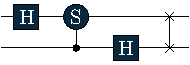
\includegraphics[width=0.4\textwidth]{src/circuit_qft_2qubits.pdf}
\end{align}
Note, that the operation $R(\pi/2)$ is often denoted as $S$ which is common for this special angle
\begin{align}
   R(\pi/2) = \begin{pmatrix}
        1 & 0 \\ 0 & i 
    \end{pmatrix} \equiv S
\end{align}

\subsubsection*{3-Qubits}
Same game as before. We have the Matrix
\begin{align}
\frac{1}{\sqrt{8}}
    \begin{pmatrix}
1 & 1 & 1 & 1 & 1 & 1 & 1 & 1 \\
1 & e^{2\pi i \frac{1}{8}} & e^{2\pi i \frac{2}{8}} & e^{2\pi i \frac{3}{8}} & e^{2\pi i \frac{4}{8}} & e^{2\pi i \frac{5}{8}} & e^{2\pi i \frac{6}{8}} & e^{2\pi i \frac{7}{8}} \\
1 & e^{2\pi i \frac{2}{8}} & e^{2\pi i \frac{4}{8}} & e^{2\pi i \frac{6}{8}} & e^{2\pi i \frac{8}{8}} & e^{2\pi i \frac{10}{8}} & e^{2\pi i \frac{12}{8}} & e^{2\pi i \frac{14}{8}} \\
1 & e^{2\pi i \frac{3}{8}} & e^{2\pi i \frac{6}{8}} & e^{2\pi i \frac{9}{8}} & e^{2\pi i \frac{12}{8}} & e^{2\pi i \frac{15}{8}} & e^{2\pi i \frac{18}{8}} & e^{2\pi i \frac{21}{8}} \\
1 & e^{2\pi i \frac{4}{8}} & e^{2\pi i \frac{8}{8}} & e^{2\pi i \frac{12}{8}} & e^{2\pi i \frac{16}{8}} & e^{2\pi i \frac{20}{8}} & e^{2\pi i \frac{24}{8}} & e^{2\pi i \frac{28}{8}} \\
1 & e^{2\pi i \frac{5}{8}} & e^{2\pi i \frac{10}{8}} & e^{2\pi i \frac{15}{8}} & e^{2\pi i \frac{20}{8}} & e^{2\pi i \frac{25}{8}} & e^{2\pi i \frac{30}{8}} & e^{2\pi i \frac{35}{8}} \\
1 & e^{2\pi i \frac{6}{8}} & e^{2\pi i \frac{12}{8}} & e^{2\pi i \frac{18}{8}} & e^{2\pi i \frac{24}{8}} & e^{2\pi i \frac{30}{8}} & e^{2\pi i \frac{36}{8}} & e^{2\pi i \frac{42}{8}} \\
1 & e^{2\pi i \frac{7}{8}} & e^{2\pi i \frac{14}{8}} & e^{2\pi i \frac{21}{8}} & e^{2\pi i \frac{28}{8}} & e^{2\pi i \frac{35}{8}} & e^{2\pi i \frac{42}{8}} & e^{2\pi i \frac{49}{8}} \\
    \end{pmatrix}
\end{align}
A common notation that makes things easier is to use the abbreviation $\omega = e^{2\pi i \frac{1}{8}} $ and realize that $\omega^8 = \omega^0 = 1$ and $\omega^9 = \omega^1$ (because $e^{2\pi i}=1$) and $\omega^4 = -1$ etc, which gives
\begin{align}
\frac{1}{\sqrt{8}}
\begin{pmatrix}
1 & 1 & 1 & 1 & 1 & 1 & 1 & 1 \\
1 & \omega^1 & \omega^2 & \omega^3 & -1 & \omega^5 & \omega^6& \omega^7 \\
1 & \omega^2 & -1 & \omega^6 & 1 & \omega^2 & -1 &\omega^6 \\
1 & \omega^3 & \omega^6 & \omega^1 & -1 & \omega^7 & \omega^2& \omega^5 \\
1 & -1 & 1 & -1 & 1 & -1 & 1 & -1 \\
1 & \omega^5 & \omega^2 & \omega^7 & -1 & \omega^1 & \omega^6& \omega^3 \\
1 & \omega^6 & -1 & \omega^2 & 1 & \omega^6 & -1 &\omega^2 \\
1 & \omega^7 & \omega^6 & \omega^5 & -1 & \omega^3 & \omega^2 & \omega^1 \\
 \end{pmatrix}.
\end{align}
We can again get the first and middle transformation correct by using a sequence of Hadamard operations followed by swapping the qubit order
\begin{align}
    \ket{000} &\rightarrow \ket{+++}\\ 
    \ket{100} &\rightarrow \ket{++-}.
\end{align}
Let's look at the transformation of the second basis state
\begin{align}
    \ket{001} &\rightarrow \frac{1}{\sqrt{8}} \left( \ket{000} + \omega^1\ket{001} + \omega^2\ket{010} + \omega^3\ket{011} - \ket{100} + \omega^5 \ket{101} + \omega^6 \ket{110} + \omega^7 \ket{111} \right)\nonumber
\end{align}
note that $\omega^2 = i$ and $\omega^6 = -i$ (so $\omega^2 = - \omega^6$) and also $\omega^5 = -\omega^1$ as well as $\omega^7 = - \omega^3$ (draw them on the complex unit circle to see it for yourself), so we have
\begin{align}
    \ket{001} &\rightarrow \frac{1}{\sqrt{8}} \left( \ket{000} + \omega^1\ket{001} + \omega^2\ket{010} + \omega^3\ket{011} - \ket{100} - \omega^1 \ket{101} - \omega^2 \ket{110} - \omega^3 \ket{111} \right)\nonumber
\end{align}
which we can further simplify to
\begin{align}
 \ket{-} \otimes \frac{1}{2}\left(\ket{00} + \omega^1\ket{01} + \omega^2\ket{10} + \omega^3\ket{11}\right).
\end{align}
Further simplification comes by realizing that $\omega^3 = \omega^1\cdot \omega^2$, so that we end up with
\begin{align}
 \ket{-} \otimes \frac{1}{\sqrt{2}}\left(\ket{0} + \omega^2 \ket{1}\right)\otimes \frac{1}{\sqrt{2}}\left(\ket{0} + \omega^1 \ket{1}\right),
\end{align}
so we are ending up with a product state again, the three individual states can be created with a Hadamard and the $R(\theta)$ operation tuned to the correct angle -- in this case we have the angles $R(\theta=\pi/4) = S$ (as before) and $R(\theta=\pi/8) = T$. To ensure that we are not messing with the $\ket{000}\rightarrow\ket{+++}$ and $\ket{100}\rightarrow\ket{++-}$ transformation we will control the two operations with the rightmost qubit and afterwards swap the qubit order again, the circuit that performs this operation is
\begin{align}
    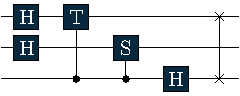
\includegraphics[height=0.1\textheight]{src/circuit_qft_3qubits_pre.pdf}.
\end{align}
With this we are almost there, there are just a few states left that are not yet transformed correctly. One of them is the last basis state should transform as
\begin{align}
    \ket{111} &\rightarrow \frac{1}{4} \left( \ket{000} + \omega^7\ket{001} + \omega^6\ket{010} + \omega^5\ket{011} - \ket{100} + \omega^3 \ket{101} + \omega^2 \ket{110} + \omega^1 \ket{111} \right)\nonumber\\
\end{align}
using our identities from before
\begin{align}
    \ket{111} &\rightarrow \frac{1}{4} \left( \ket{000} + \omega^7\ket{001} + \omega^6\ket{010} + \omega^5\ket{011} - \ket{100} - \omega^7 \ket{101} - \omega^4 \ket{110} - \omega^7 \ket{111} \right)\nonumber\\
    &= \ket{-} \otimes \frac{1}{2}\left( \ket{00} + \omega^7\ket{01} + \omega^6\ket{10} + \omega^5\ket{11}\right).
\end{align}
Now, remember the periodicity again and realize that $\omega^7 \cdot \omega^6 = \omega^{13} = \omega^5$
\begin{align}
    \ket{111} &\rightarrow \ket{-}\otimes \frac{1}{\sqrt{2}}\left(\ket{0} + \omega^6\ket{1}\right)\otimes\frac{1}{\sqrt{2}}\left(\ket{0} + \omega^7\ket{1}\right)
\end{align}
or, in our case more convenient
\begin{align}
    \ket{111} &\rightarrow \ket{-}\otimes \frac{1}{\sqrt{2}}\left(\ket{0} - \omega^2\ket{1}\right)\otimes\frac{1}{\sqrt{2}}\left(\ket{0} - \omega^3\ket{1}\right).
\end{align}
This is almost the same state as we already had above for the $\ket{001}$ transformation, except for the minus signs (they will however be correctly introduced by the Hadamard transformations, now acting on qubits in $\ket{1}$ and not $\ket{0}$) and the frequency in the rightmost qubit which is $\omega^3$ instead of $\omega^1$. To get the correct frequency we can modify the circuit with an additional controlled-$S$ operation (note that $S$ acting on $\omega^1\ket{1}$ will lead to $\omega^2\omega^1\ket{1 = \omega^3\ket{1}}$). We place the control on the central qubit (so the operation will be switched off in the $\ket{001}$ transformation above). 
The final circuit for the 3-Qubit \textsc{QFT} is then
\begin{align}
    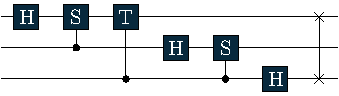
\includegraphics[height=0.1\textheight]{src/circuit_qft_3qubits.pdf},
\end{align}
this circuit transforms all states correctly -- verification on the remaining 4 states is left as an exercise.

\subsection*{N-Qubits}
\begin{algo*}[\texttt{QFT}]\phantom{...}\\
The circuit for the quantum Fourier transform on $N$ qubits can be assembled
\begin{algorithmic}
\STATE $\textsc{qft} = \left[\right] $
\FOR{$ 1 \leq n \leq N$}
\STATE $ \texttt{qft} += \hd(n) \texttt{qft} $
\FOR{$1\leq m \leq  N-n$}
\STATE $ \texttt{qft} += CR\left(n+m,n,\frac{\pi}{2^{m+1}}\right)$
\ENDFOR
\ENDFOR
\FOR{$1 \leq n \leq $ $ \lfloor{N/2}\rfloor$}
\STATE $\texttt{qft} += \texttt{SWAP}(n,N-(n-1))$
\ENDFOR
\RETURN $\texttt{qft}$
\end{algorithmic}
Here we used "$+=$" to indicate the assembling of gates in a list. 
\end{algo*}

\clearpage
\newcommand{\Mod}[1]{\ (\mathrm{mod}\ #1)}
\DeclarePairedDelimiter{\ceil}{\lceil}{\rceil}
\newcommand\scalemath[2]{\scalebox{#1}{\mbox{\ensuremath{\displaystyle #2}}}}

\section{Shor's Factoring Algorithm}
% rename this section as you like, e.g. Applications of QFT, ...

In 1995, Peter Shor introduced a quantum algorithm that efficiently solves the integer factoring problem, i.e., decomposing large numbers into their prime factors in polynomial time. This was groundbreaking because factoring is believed to require exponential costs on a classical computer, which is why it became the basis of widely used cryptographic systems like RSA encryption\footnote{In fact, cryptographic standards are now evolving in response to the potential threat posed by quantum computers capable of running Shor’s algorithm.}. The implications of Shor's work are therefore enormous: Not only does it demonstrate a concrete case of practical quantum advantage, but it also provides a credible challenge to the strong Church-Turing thesis\footnote{in simple words, the thesis states that all efficient algorithms can be reduced to (probabilistic) Turing machines. Shor's Algorithm challenges the thesis since a quantum computer can efficiently factor primes, but to this day, there is no efficient classical algorithm. The prime-factoring problem is in fact a candidate for an $NP$-Intermediate problem -- conjectured to be neither $NP$-complete nor in $P$.}. This finding catalyzed the modern field of quantum computing, spurring both theoretical research and the development of actual quantum hardware. 

At its core, Shor’s algorithm is just a clever application of the quantum phase estimation \texttt{QPE} that includes the quantum Fourier transform \texttt{QFT} as a subalgorithm (see previous chapters). It relies on the observation that the factoring problem can be reduced to the order finding problem, which can be efficiently solved with \texttt{QPE}.

The quantum part of Shor's algorithm solves the order-finding problem. We will start with this and will then see how order-finding is used for integer factoring.

\subsection{Order-Finding}
Let us consider the following arithmetic problem.
\begin{def*}[Order-Finding]
Suppose an odd, composite number $N>1$ which is not a prime power, and an integer $x<N$, which is \textit{coprime} to $N$, i.e., $x$ and $N$ have no common factors. Determine the least positive integer $r$ such that ${x^r =1\Mod{N}}$. 
\end{def*}
In order words: At what order $r$ does the sequence ${x^1\Mod{N}},\ {x^2\Mod{N}}, ...$ reach the value $1$? As a simple example, consider the following: 
\begin{ex*}[$N=5$, $x=3$]
The coprime integers $N=5$ and $x=3$ give the sequence
\begin{align*}
 &3^1\Mod{5}= 3\Mod{5}= 3,\quad 3^2\Mod{5}= 9\Mod{5}= 4,\\
 &3^3\Mod{5}= 27\Mod{5}= 2, \quad 3^4\Mod{5}= 81\Mod{5}= 1, \quad \dots
\end{align*}
which tells us that the order of $3$ modulo $5$ is $4$. 
\end{ex*}

While this might seem easy to solve at first, note that for large integers, the value of $r$ can be very large, making an enumeration strategy like the one above highly impractical. In fact, order-finding is believed to be hard on classical computers, meaning that no known algorithm can solve it using only polynomial resources in $L\equiv\ceil{\log{N}}$, which is the number of bits encoding $N$. 

Instead, Shor proposed to solve this problem efficiently using quantum phase estimation (\texttt{QPE}) applied to the unitary operator
\begin{equation}
    U\ket{{y}} = \ket{{x}{y}\Mod{N}},
\end{equation}
where $\ket{{y}}$ denotes the basis state corresponding to the bit string encoding the integer $y$, with $0\leq y\leq N-1$. The states given by
\begin{equation}
    \left|u_s\right\rangle \equiv \frac{1}{\sqrt{r}} \sum_{k=0}^{r-1} \mathrm{e}^{-2 \pi \mathrm{i} k\frac{s}{r}}\ |x^k \Mod{N}\rangle,
\end{equation}
for integers $0\leq s\leq r-1$, are the eigenstates of $U$ with eigenvalues $\mathrm{e}^{2 \pi \mathrm{i} \frac{s}{r}}$. To show this, consider the following calculation:
\begin{equation}
\begin{aligned}
 U\left|u_s\right\rangle 
 & =\frac{1}{\sqrt{r}} \sum_{k=0}^{r-1}\ \mathrm{e}^{-2 \pi \mathrm{i} k\frac{s}{r}}\ |x^{k+1} \Mod{N}\rangle \\
& =\frac{1}{\sqrt{r}} \sum_{k=0}^{r-1}\ \mathrm{e}^{2 \pi \mathrm{i} \frac{s}{r}} \mathrm{e}^{-2 \pi \mathrm{i} (k+1)\frac{s}{r}}\ |x^{k+1} \Mod{N}\rangle \\
& \stackrel{(*)}{=} \mathrm{e}^{2 \pi \mathrm{i} \frac{s}{r}}\: \frac{1}{\sqrt{r}} \sum_{\tilde{k}=1}^r \mathrm{e}^{-2 \pi \mathrm{i} \tilde{k}\frac{s}{r}}\ |x^{\tilde{k}} \Mod{N}\rangle\qquad&\scalemath{0.8}{(*)\ \tilde{k}=k+1}\\
& \stackrel{(**)}{=}\mathrm{e}^{2 \pi \mathrm{i} \frac{s}{r}}\: \frac{1}{\sqrt{r}} \sum_{\tilde{k}=0}^{r-1} \mathrm{e}^{-2 \pi \mathrm{i} \tilde{k}\frac{s}{r}}\ |x^{\tilde{k}} \Mod{N}\rangle\qquad&\scalemath{0.8}{(**)\ \mathrm{periodicity\ w.r.t\ }r}\\
& =\mathrm{e}^{2 \pi \mathrm{i} \frac{s}{r}}\left|u_s\right\rangle
\end{aligned}
\end{equation}

This means that given the unitary $U$, an efficient procedure to implement controlled-$U^{2^j}$ operations\footnote{Note that this can be realized by a procedure called \textit{modular exponentiation} requiring $\mathcal{O}(L^3)$ gates.} for any $j$, and the corresponding eigenstate $\ket{u_s}$, we would be able to apply \texttt{QPE} to get the phase $\frac{s}{r}$ of the corresponding eigenvalue. Problem solved? Unfortunately, there is an issue: Preparing the state $\ket{u_s}$ requires prior knowledge of the value of $r$, which is precisely what we want to determine. However, we can circumvent this problem using the clever observation that the uniform superposition of all eigenstates satisfies\footnote{See Exercise sheet for a proof.}
\begin{equation}
\frac{1}{\sqrt{r}} \sum_{s=0}^{r-1}\left|u_s\right\rangle=|\mathbf{1}\rangle,
\end{equation}
which means we do not need to explicitly prepare $\ket{u_s}$. Instead, we can simply initialize the second register in the \texttt{QPE} algorithm in the easily prepared state $\ket{\mathbf{1}}$\footnote{Remember: $\ket{\mathbf{1}}$ denotes the computational basis state corresponding to the bit string $0\dots01$ of length $L$.}. As a result, when the \texttt{QPE} algorithm is executed, the first register collapses to an estimate of $\frac{s}{r}$ where $s\in\{0,\dots,r-1\}$ is chosen approximately uniformly at random. Since we are ultimately interested in the denominator $r$ rather than the particular value of $s$, this randomness does not affect the outcome. Further notice that by repeated applications of the unitary operator $\ket{U}$ to the state $\ket{1}$, we get 
\begin{equation}
    U^j\ket{1} = \ket{x^j\Mod{N}},
\end{equation}
which exactly reproduces the elements of the periodic sequence we are trying to analyze.

The quantum algorithm for order-finding is finally summarized as follows.

\begin{algo*}[\texttt{QPE} for Order-Finding]\phantom{...}\\
The following quantum circuit can be used to obtain an estimate for the phase $\frac{s}{r}$ given the state $\ket{1}$ and operator $U$ as defined above.
\begin{center}
\begin{quantikz}
\lstick{$\ket{0}$} & \qwbundle{n} & \gate{H^{\otimes n}} & \ctrl{1} & 
\gate{\texttt{QFT}^\dagger} & \meter{} \rstick{$\approx\frac{s}{r}$} \\
\lstick{$\ket{1}$} & \qwbundle{L} & \qw & \gate{ U^j } & 
\qw & \qw
\end{quantikz}
\end{center}
\end{algo*}
Note that the number of qubits in the first register determines the precision of our phase estimate. Specifically, if we choose
\begin{equation}
    n = 2L+1+\ceil[\Bigg]{\log(2+\frac{1}{2\epsilon})},
\end{equation}
then, for each $s\in\{0,\dots,r-1\}$, the above algorithm yields an estimate $\tilde{\varphi}$ of $\frac{s}{r}$ accurate to at least $2L+1$ bits, with success probability at least $\frac{1-\epsilon}{r}$. Once we have such an estimate $\tilde{\varphi}$, we can recover the exact value of the desired order parameter $r$ using the \textit{continued fractions} algorithm\footnote{see Tutorial for details on this procedure.}. With this final step, we have completed the reduction of order-finding to quantum phase estimation.

\subsection{Factoring}
The order-finding problem is computationally equivalent to the problem of factoring.
\begin{def*}[Factoring]
%Given a positive composite number $N$, what are the prime numbers -- when multiplied together -- equal it?
Given a positive composite number $N$, what are the prime numbers $X_1,X_2,\dots$ such that $\prod_k X_k = N$.
\end{def*}
This means that any efficient algorithm for order-finding can be straightforwardly transformed into an efficient factoring algorithm. The reduction from factoring to order-finding is based on two key properties:

\begin{theorem*}
Given an $L$-bit composite integer $N$, and suppose $x$ with $1\leq x\leq N$ satisfies
\begin{equation}
x^2=1\Mod{N},
\label{eq:modexp}
\end{equation}
but $x\neq \pm 1 \Mod{N}$. Then at least one of $\texttt{gcd}(x-1,N)$ and $\texttt{gcd}(x+1,N)$ is a non-trivial factor of $N$, computable using $\mathcal{O}(L^3)$ operations.
\end{theorem*}
This means that if we manage to find a non-trivial solution $x$ to \eqref{eq:modexp}, then we can compute a non-trivial factor of $N$, namely the greatest common divider ($\texttt{gcd}$) of $x\pm1$ and $N$.

\begin{theorem*}
Given an odd composite integer $N$ and its $m$ distinct prime factors. Let $x$ be a random integer chosen uniformly from $1,\dots, N-1$ such that $x$ is coprime to $N$, i.e., $\texttt{gcd}(x,N)=1$. Let $r$ be the order of $x$ modulo $N$. Then the probability of $r$ being even and 
\begin{equation}
    x^{\frac{r}{2}}\neq \pm 1 \Mod{N}
    \label{eq:modexp2}
\end{equation}
is at least $1-1/2^m$.
\end{theorem*}
This second theorem implies that if we chose a random number $y<N$, coprime to $N$, it is quite likely to have an order $r$ which is even and satisfies \eqref{eq:modexp2}. Linking this statement to the first property, we get that $x\equiv y^{\frac{r}{2}}\Mod{N}$ is a solution to \eqref{eq:modexp}.

Combining these considerations results in Shor's algorithm for integer factoring.
\begin{algo*}[Shor's Factoring Algorithm]\phantom{...}\\
Given a composite integer $N$, output a non-trivial factor of $N$.

\begin{algorithmic}
\STATE \textbf{if} $N \Mod{2} = 0$ \textbf{return} $2$ \hfill // check if $N$ is even
\STATE \textbf{if} $N = a^b$ for some $a \geq 1$, $b \geq 2$ \textbf{return} $a$ \hfill // check if $N$ is perfect power
\STATE \textbf{repeat}
\STATE $\quad x \gets$ random integer in $[1, N - 1]$
\STATE $\quad g \gets \texttt{gcd}(x, N)$
\STATE $\quad$\textbf{if} $g > 1$ \textbf{return} $g$
\STATE $\quad$\textbf{else}
\STATE $\quad\quad r \gets \texttt{QPE}$ for Order-Finding of $x$, $N$
\STATE $\quad\quad$\textbf{if} $r\Mod{2} = 0$ \textbf{and} $x^{r/2}\neq \pm 1\Mod{N}$ \textbf{do} $y \gets x^{r/2} \Mod{N}$
\STATE $\quad\quad\quad$\textbf{if} $y = 1$ \textbf{or} $y = N - 1$ \textbf{continue}
\STATE $\quad\quad\quad$\textbf{else}
\STATE $\quad\quad\quad\quad f_1 \gets \texttt{gcd}(y - 1, N)$
\STATE $\quad\quad\quad\quad f_2 \gets \texttt{gcd}(y + 1, N)$
\STATE $\quad\quad\quad\quad$\textbf{if} $1 < f_1 < N$ \textbf{return} $f_1$
\STATE $\quad\quad\quad\quad$\textbf{if} $1 < f_2 < N$ \textbf{return} $f_2$
\STATE $\quad\quad$\textbf{else} \textbf{continue}
\end{algorithmic}
\end{algo*}
The first two lines of preprocessing ensure that $N$ is an odd composite integer with more than one prime factor. This can be done using standard classical routines in $\mathcal{O}(1)$ and $\mathcal{O}\left(L^3\right)$ time. In the main step of the algorithm, we either immediately find a factor from a randomly selected element $x \in\{1, \ldots, N-1\}$ or we continue with the quantum order-finding subroutine from the previous section to compute the order $r$ of $x$ $\Mod{N}$. Using the above properties, we then attempt to extract a non-trivial factor of $N$ from $r$. This succeeds with probability at least $\frac{1}{2}$ for each iteration, provided $r$ is even and $x^{r / 2} \not \equiv \pm 1 \Mod{N}$.

Lastly note that all parts of this algorithm can be executed efficiently on a classical computer except for the order-finding subroutine, which is where the quantum advantage lies.

\clearpage

\section{Quantum Computational Complexity}\label{chap:complexity}
The theory of computational complexity centres around the question what the minimal required resources to solve a given computational problem are. Although one can discuss about different resources, time, space, energy, let us focus here on the specific question of (run)time required to solve a given problem.

Summing up two n-bit numbes takes $O(n)$, while mutiplication takes in principle $O(n \log n)$. Search in a structured data base takes $O(\log n)$.
\footnote{We say the function $f(n)$ is in the class of functions $O(g(n))$ if at some point the function $g(n)$ scaled by an arbitrary constant grows faster than $f(n)$. Formally this can be defined as
\begin{align*}
    O(g(n)) = \left\{f(n) \;|\; \exists n_0\in\mathbb{N}, \forall c\in\mathbb{N}, \forall n\geq n_0: f(n)\leq c\cdot g(n)\right\}
\end{align*}
we will however not need the formal definition. }
The big-O is essentially the ``smaller as'' for functions, meaning $f\in O(g)$ can be read as ``$f$ is asymptotically smaller than $g$''.~\footnote{in the same way we have $f\in \Omega(g)$ for $f$ larger $g$ and $f\in\Theta(g)$ for $f$ equal $g$} 

We can then classify the problems as tractable problems, which can be solved in polynomial time, and intractable problems, which are superpolynomial -- where superpolynomial just means that a function grows larger than any polynomial. An exponential function is for example superpolynomial (but not all superpolynomial functions are exponential).~\footnote{for this course it is fine to just think about polynomial and exponential though}
To classify tractable problems, the complexity class $\mathrm{P}$ was introduced. \\

The classical complexity classes below are all formally defined for Turing machines -- which you can just view as ``classical computer''.
Here is a very simple example of a Turing machine: consider the problem of determining if a given integer is odd or even, we can call it $\texttt{even}(n)$. We can encode integers in binary, meaning we can use the alphabet $\Sigma=\left\{0,1\right\}$ to form words that represent integers. We can now write the binary representation of any integer onto the tape of a Turing machine and let the machine figure out if the integer is even -- if it is even, the machine will accept. All the machine needs to do, is to move to the end of the input string and check if it is the symbol 0 -- if so, then the machine can accept, otherwise it just halts (or rejects). If the string consists of $O(N)$ symbols, then this takes roughly $O(N)$ elementary transitions for the machine. Therefore the problem is solved in polynomial time on a Turing machine, and we have $\texttt{even}\in \mathrm{P}$. Note here that the choice of a binary alphabet is kind of arbitrary. We could have also used decimal representation with the alphabet $\Sigma=\left\{0,1,2,3,4,5,6,7,8,9\right\}$. Then, the machine needs to move to the last entry of the input and check if it is any of the symbols $0,2,4,6,8$. So, the machine needs to have some more transitions defined, but the actual runtime will stay linear.\\
If we change the encoding of our integer to "least significant bit first" then it will only take a single step for a suitable Turing machine (simply just checking if the first bit is 0). The same is true if we take a Random Access Machine (a different model of computation) that is able to directly access datafields. Since the computers we use are closer to Random Access Machines.

\subsection{Complexity Classes}

Besides the problems that can be solved efficiently, we can also form two more classes, where we don't necessarily know if we can solve efficiently, but where we at least can certainly verify a given solution efficiently.

\begin{def*}[Basic Complexity Classes]\phantom{...}
\begin{align*}
\mathrm{P} &: \text{efficient algorithm}\\
\mathrm{NP}&: \text{efficient verification with short proofs}\\
\mathrm{coNP} &: \text{efficient falsification with short proofs}     
\end{align*}
\end{def*}
Efficient means that there exists an algorithm that runs in polynomial time w.r.t the length of the original instance of the problem. A short proof is an additional input whose length is polynomially bounded by the length of the original instance of the problem.
Here are some examples:\\

$\texttt{SubsetSum}(I,c)$: given natural numbers $I=\left\{n_1,n_2,\dots n_N\right\}$ determine if there is a subset $S\subseteq I$ such that the numbers in $S$ add up to $c$. We have that $\texttt{SubsetSum}\in \mathrm{NP}$ since we can efficiently verify: If the instance is true then a subset $S$ with the requested properties has to exist. If given such a subset $S$ (this is the short proof) it is easy to check if it is a subset of $S$ and the numbers indeed add up to $c$ (this is the verification). On the other hand: It is unclear if we can also easily falsify the problem, meaning if the answer is no, we don't know how to proof that efficiently -- the problem is most likely not in $\mathrm{coNP}$. We also don't know how to solve the problem, and it is most likely not in $\mathrm{P}$.\\

$\texttt{Taut}(\varphi)$: Determine if a given Boolean function is a tautology (meaning if it is constant 1). We have $\texttt{Taut}\in \mathrm{coNP}$ because it is easy to falsify: if the answer is no, it suffices to provide a variable assignment that evaluates to false. On the other hand, we don't know how to verify the problem: if the answer is yes, it is hard to efficiently verify that the function is indeed a tautology. And similarly we don't know how to efficiently decide the problem.\\

\texttt{Factoring}$(n)$: Decompose a given integer $n$ into its prime factors. The decision version is \texttt{Factor}$(n,m)$: Determine if there is a $k\leq m$ that is a factor of $n$. We have $\texttt{Factor}\in \mathrm{NP}$ since we can easily verify (provide the answer and check if it is indeed a factor of $n$). But we also have $\texttt{Factor}\in \mathrm{coNP}$ because we can also easily verify: if there is no factor of $n$ smaller than $m$ we can provide the prime-factorization of $n$ and check that all factors are larger than $m$.~\footnote{non-trivial structure: the fundamental theorem of arithmetic guarantees us that each integer $n$ has a unique factorization using prime numbers. It is also possible to efficiently check if a given number is a prime number (AKS-primality test).}

\begin{def*}[Complete Problems] If a decision problem is complete for a class, it essentially means that all other problems within that class can be efficently transformed into instances of the complete problem. The complete problems in $\mathrm{NP}$ and $\mathrm{coNP}$ form the classes $\mathrm{NPC}$ and $\mathrm{coNPC}$. Examples (without proofs):
\begin{align*}
    \texttt{SAT} \in \mathrm{NPC}\\
    \texttt{Taut} \in \mathrm{coNPC}
\end{align*}
but also $\texttt{SubsetSum} \in \mathrm{NPC}$ and many more. If we find an efficient algorithm to decide a problem in $\mathrm{NPC}$ then we can efficiently decide \textit{all} problems in $\mathrm{NP}$ (and additionally all problems in $\mathrm{coNP}$). 
\end{def*}
Note that it is not known if $\texttt{Factor}$ is complete for $\mathrm{NP}$ (or $\mathrm{coNP}$) but it is generally assumed that this is not the case. 



\subsection{Quantum Complexity Classes}

\begin{def*}[Basic Quantum Complexity Classes]
\begin{align*}
    {\mathrm{BQP}} &: \text{efficient quantum algorithm}\\
    {\mathrm{QMA}} &: \text{efficient quantum verification with short quantum proof}
\end{align*}
\end{def*}

These classes are basically the analogues of $\mathrm{P}$ and $\mathrm{NP}$ with the difference that a small error probability is required. For $\mathrm{BQP}$ it means that the algorithm is only required to give the correct answer with a probability of at least 2/3,~\footnote{this is the $B$ in $\mathrm{BQP}$ which stands for bounded probability.} and similar for $\mathrm{QMA}$ where the 2/3 bound holds for the verification.~\footnote{the names originate from $\mathrm{BPP}$ and $\mathrm{MA}$, which are the probabilistic versions of $\mathrm{P}$ and $\mathrm{NP}$.} The latter works in the following way: A decision problem $A$ is in $\mathrm{QMA}$ if for every instance $x$ of the problem, we can construct a circuit $U_x$ that takes an arbitrary quantum state $\ket{\phi}$ as input and outputs a final measurement on a designated qubit. For the circuit $U_x$ it needs to hold that iff $A(x)=1$ (the instance is true), then a state $\ket{\phi}$ (a ``proof'') exists such that $U_x\ket{\phi}$ gives at least 2/3 chance to read out 1 on the designated read-out qubit. With short quantum proof, we mean that the proof state $\ket{\phi}$ can only be defined on a number of qubits that is polynomially bounded by the length of the original instance $x$. Lets see an example:\\

\texttt{GroundState}$(H, \mu)$: Determine if the smallest eigenvalue $E_0$ of Hamiltonian $H$ is below the threshold $\mu$. We show that $\texttt{GroundState}\in \mathrm{QMA}$. First: Since $H$ is Hermitian is has real eigenvalues (if $H$ is defined on $N$ qubits, there are exactly $2^N$ eigenvalues) and one of them is the lowest. For the lowest eigenvalue $H\ket{E_0} = E_0 \ket{E_0}$ there is also an eigenstate $\ket{E_0}$. We can use this eigenstate as proof and the quantum-phase estimation algorithm as verifyier.~\footnote{See quantum algorithms lecture for details on quantum phase estimation. If unknown: See the ``in a nutshell'' version after this chapter}  

\begin{figure}
    \centering
    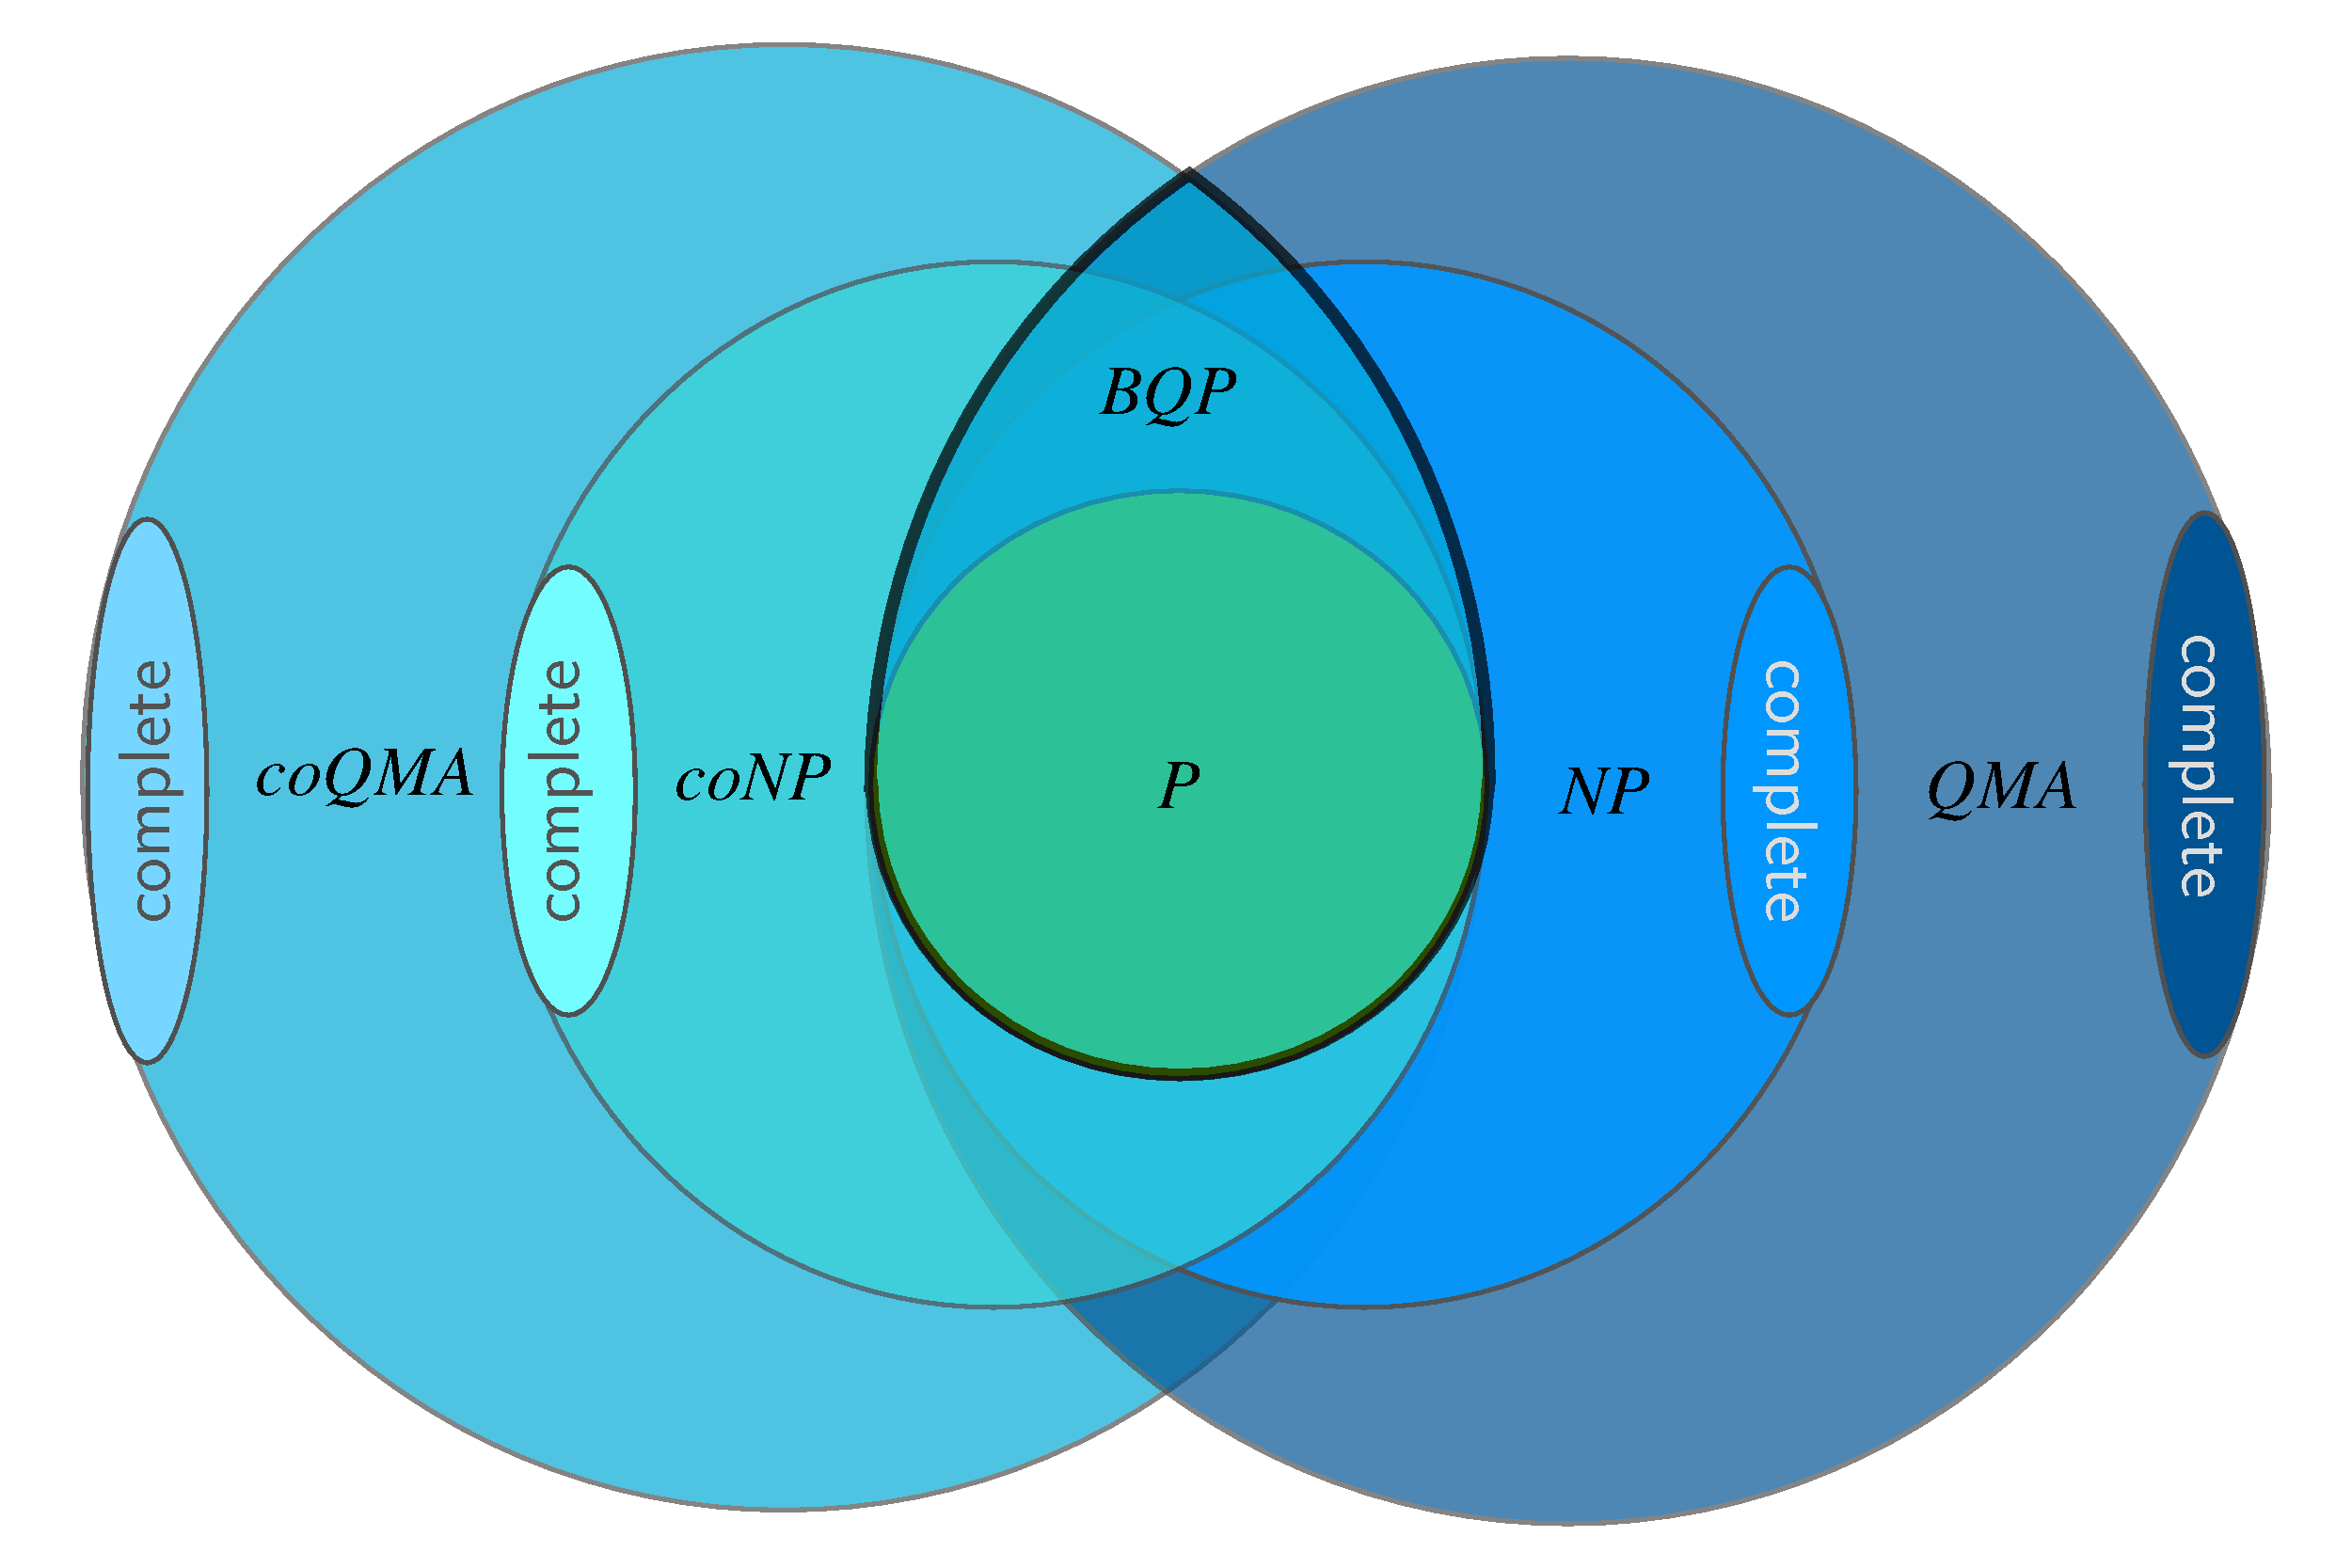
\includegraphics[width=0.85\linewidth]{src/complexity-classes-1.pdf}
		\caption{Complexity-Classes: Sketch of current assumptions. Known inclusions are: $\mathrm{P}\subseteq \mathrm{(co)NP} \subseteq \mathrm{(co)QMA}$ and $\mathrm{BQP}\subseteq \mathrm{(co)QMA}$. The rest of the sketch is conjectured but not proven.}
    \label{fig:complexity-classes}
\end{figure}

\begin{def*}[$\mathrm{QMA}$ Complete Problems] In the same way as for $\mathrm{NP}$-complete problems, we have $\mathrm{QMA}$ complete problems. Here, the most prominent one is the groundstate problem
\begin{align*}
    \texttt{GroundState} \in \mathrm{QMA}\text{-complete}
\end{align*}
\end{def*}
It turns out that not only is \texttt{GroundState} $\mathrm{QMA}$-complete, but also several restricted versions. It suffices for example to have a ``local'' Hamiltonian $H=\sum_i c_i h_i$, where the ``small'' Hamiltonians $h_i$ only act on a locally restricted part of the system -- in qubit language a $k$-local Hamiltonian can be represented like this, with all $h_i$ only acting on $k$ qubits of the total system.
For the $\mathrm{QMA}$ completeness it suffices to be 2-local, so these problems are already hard.

\subsection{Kitaev's Clock and QMA-Hardness} 
Here we will give an illustration about the main idea behind Kitaev's idea to show $\mathrm{QMA}$ hardness of \texttt{Groundstate}. We will try to focus on the key idea ommiting the nitty-gritty.\\

A quantum algorithm essentially works like this:
\begin{enumerate}
    \item prepare an initial basis state (or use the convention that we always start with $\ket{0}^N$
    \item apply a sequence of quantum gates $U_n\dots U_2U_1$
    \item read-out one (or multiple) qubits
\end{enumerate}
So the ``history'' of the computation is as follows
\begin{align}
    \ket{\psi_0} &= \ket{\mathbf{0}} \equiv \ket{0}^N\\
    \ket{\psi_1} &= U_1\ket{\psi_0}\\
    \vdots &\\
    \ket{\psi_i} &= U_i \ket{\psi_{i-1}} = U_i U_{i-1}\dots U_2U_1\ket{\psi_0}.
\end{align}
Going back to Feynman (and later Kitaev) we can define a ``history-state'' that contains all points of the computation
\begin{align}
    \ket{\Psi} = \frac{1}{\sqrt{n+1}}\left( \ket{\mathbf{0}}\otimes \ket{\mathbf{0}} + \sum_{k=1}^n \ket{\mathbf{k}} \otimes \ket{\psi_k} \right)
\end{align}
here, we added a second qubit register with $\lfloor \log_2(n)\rfloor + 1$ qubits that acts as an index for the individual epochs in the history of the computation.
We will now construct a Hamiltonian, such that the history state is it's groundstate with energy zero. This can be achieved as
\begin{align}
    H = H_0 + H_c +  H_n
\end{align}
using $H_0$ to ``fix'' the initial state, $H_c$ to encode the computation, and $H_n$ to encode the result. 
In our example, the initial state is supposed to be $\ket{\mathbf{0}}$, so we can just create a projector
\begin{align}
    H_0 = \ket{\mathbf{0}}\bra{\mathbf{0}} \otimes \left(1-\ket{\mathbf{0}}\bra{\mathbf{0}}\right)
\end{align}
so for the history state, we have
\begin{align}
    H_0 \ket{\Psi} = 0 \ket{\Psi}
\end{align}
and all other states with nonzero overlap with $\ket{\mathbf{0}}\otimes \ket{\psi}$ where $\braket{\mathbf{0}}{\psi}=0$ this will add a non-zero ``punishment''. This Hamiltonian alone does not distinguish between the history state and any other state that does not overlap with $\ket{\mathbf{0}}\otimes \ket{\psi}$ as given above. This is why the other two Hamiltonians are also needed. 
The computation can be encoded with 
\begin{align}
    H_c = \sum_{k=1}^{n-1} \ket{\mathbf{k}}\bra{\mathbf{k}}\otimes 1 + \ket{\mathbf{k}+1}\bra{\mathbf{k}+1}\otimes 1 - \ket{\mathbf{k}}\bra{\mathbf{k}+1} \otimes U^\dagger_{k} - \ket{\mathbf{k}+1}\bra{\mathbf{k}} \otimes U_{k}
\end{align}
because $U_k$ is the transition between the $k$th and $k+1$ step in the computation, while $U_k^\dagger$ is the inverse part. For the history state the two positive terms will cancel with the negative ones leading to an eigenvalue of zero.
In the end, we can also encode the desired output
\begin{align}
    H_n = \ket{\mathbf{n}}\bra{\mathbf{n}}\otimes P
\end{align}
where $P=\ket{0}\bra{0}\otimes 1\otimes 1\otimes \dots $ is a projector that adds a punishment if the circuit does not accept (i.e. if the designated output qubit is not in $\ket{1}$ at the end of the computation).\\

Through this construction we have the following equivalence: If the quantum algorithm $U_nU_{n-1}\dots U_2U_1\ket{0}$ accepts (i.e. the output qubit will be in $\ket{1}$) then the clock-Hamiltonian will have lowest eigenenergy zero and vice versa.\\

The previous illustration contains the main ideas that show the $\mathrm{QMA}$ hardness of \texttt{Groundstate}. Some comments to connect to the actual $\mathrm{QMA}$ hardness result
\begin{itemize}
    \item Instead of looking at a designated quantum algorithm that starts from $\ket{\mathbf0}$, we need to look at a quantum verifier -- a quantum circuit that can take an arbitrary $N$-qubit state (the certificate) as input. Essentially we just need to change $H_0$ (such that we do nothing on the input qubits that encode the quantum verifyier) for that.
    \item In order to show that local Hamiltonians (5-local in the original proof by Kitaev) we need to use a different encoding for the clock-register. Instead of $O(\log n)$ qubits, we can just use $n+1$ qubits and use unary encoding: $\ket{\mathbf{0}}=\ket{000\dots}, \ket{\mathbf{1}}=\ket{100\dots}, \ket{\mathbf{2}}=\ket{010\dots }, \ket{\mathbf{3}}=\ket{001\dots}$)
    \item $\mathrm{QMA}$ verification is probabilistic, i.e. it suffices if the circuit accepts with probability larger than 2/3 for a valid certificate. This needs to be considered. At the end you have something like: If there is a certificate such that the verifyier accepts with probability $1-\epsilon$, then the clock Hamiltonian has a groundstate close to zero, with some tolerance depending on $\epsilon$.
\end{itemize}

\clearpage
\section{Variational Quantum Algorithms}

Variational (quantum) algorithms are a broad subclass of algorithmic approaches towards the groundstate problem from many-body chemistry and physics. 
\begin{def*}[Groundstate Problem]
Given a (sparse) Hamiltonian $H$ -- estimate the lowest eigenvalue. Optional: estimate the corresponding eigenvector
\end{def*}
In this course, we will focus on variational algorithms designed for quantum computers -- often called variational quantum algorithms (VQA), variational quantum eigensolvers (VQE), or quantum approximate optimization algoritjms (QAOA). 
There are however many other applications that employ the same principles. To name a few:
\begin{itemize}
    \item Density Functional Theory (DFT) -- the ``powerhouse'' of computational chemistry is based on variational algorithms (although DFT itself is not variational with respect to the original many-body Hamiltonian anymore, it is still variational with respect to the fixed energy functional)
    \item QAOA - the quantum approximate optimization algorithm, designed to solve combinatorical problems on quantum computers
    \item Many top notch algorithms from classical quantum chemistry: Configuration interaction (CI), Density matrix renormalization group (DMRG), other types of tensor networks, neural quantum states.
\end{itemize}
It is at this point not necessary nor required to know any of the above acronyms. However, you might encounter one of those at some point and maybe remember some of the basics about variational algorithms. 

\subsection{Expectation Values}
An expectation value (or ``expected value'') of an observable given by the Hermitian matrix $H$ with respect to a quantum state $\ket{\psi}$ is just the average result that you would get over repeated measurements. Meaning if you implement the protocol:
\begin{enumerate}
    \item Prepare the state $\ket{\psi}$
    \item Measure observable $H$, collect the obtained eigenvalue $E_i$
    \item Repeat $n$ times and build the average: $\sum_{k=1}^n E_{i_k}/n$ 
\end{enumerate}
As our observables are usually Hamiltonians (i.e. the ``energy'' of a system) we will denote the eigensystem as
\begin{align}
    H\ket{E_i} = E_i \ket{E_i},
\end{align}
and will further always assume that the eigenvalues are ordered: $E_0 \leq E_1 \leq E_2\leq \dots $.
At this point, it's again useful to re-iterate the sections on eigensystems of Hermitian matrices ($E_i\in \mathbb{R}$ and $\braket{E_i}{E_j}=\delta_{ij}$ in the appendix.
\begin{def*}[Expectation Value] For a given observable $H$ and quantum state $\ket{\psi}$ the expectation value of the observable w.r.t the state is
\begin{align} 
    \langle H \rangle_\psi := \bra{\psi}H\ket{\psi},
\end{align}
\end{def*}
To see why this is indeed the result of the protocol above with $n\rightarrow \infty$ we represent the state $\ket{\psi}$ in the eigenbasis of $H$
\begin{align}
    \ket{\psi} = \sum_{i} c_i \ket{E_i}
\end{align}
with $c_i=\braket{E_i}{\psi}$ the probability amplitude that we observe the system in eigenstate $\ket{E_i}$. If we plug this into the definition above we get
\begin{align} 
     \bra{\psi}H\ket{\psi} &= \sum_{ij} c_i^* c_j \bra{E_i}H\ket{E_j}\nonumber\\
     &= \sum_{ij} c_i^* c_j \bra{E_i}E_j\ket{E_j}\nonumber\\
      &= \sum_{ij} c_i^* c_j E_j \delta_{ij}\nonumber\\
       &= \sum_{ij} |c_i|^2 E_i\nonumber\\
\end{align}
so this is just a sum over all possible eigenvalues weighted by the probability to observe them.
\vspace{0.5cm}
\noindent\rule{\textwidth}{0.4pt}
\vspace{0.5cm}
Example: Let's look at a simple Observable given by the Pauli-Z matrix
\begin{align}
Z = \begin{pmatrix}
    1 & 0\\ 0 & -1
\end{pmatrix}
\end{align}
its eigenstates are just the standard basis states of a single qubit with eigenvalues $+1$ for $\ket{0}$ and $-1$ for $\ket{1}$. Let's consider a single qubit in the symmetric superposition of the two basis states, namely the $\ket{+} = \frac{1}{\sqrt{2}}\left(\ket{0}+\ket{1}\right)$ state. If we measure the observable given by $Z$ we either get $+1$ or $-1$, each with a probability of $\frac{1}{2}$. We can directly see that the expected value is the average result over infinite repetitions -- in this case the average result will be 0 as $+1$ and $-1$ are obtained with equal probabilities. Let's check via the definition by simply applying the matrix $Z$ to the state $\ket{+}$ and then take the inner product with $\bra{+}$:
\begin{align}
    \expval{Z}_{+} &= \bra{+}Z\ket{+} = \bra{+}\frac{1}{\sqrt{2}}\left(Z\ket{0} + Z\ket{1} \right) \\
    &= \bra{+} \frac{1}{\sqrt{2}}\left( \ket{0} - \ket{1}\right) = \braket{+}{-} = 0.
\end{align}
So we arrive at the result we intuitively suspected -- remember that the states $\ket{\pm}$ are orthogonal.
\vspace{0.5cm}
\noindent\rule{\textwidth}{0.4pt}
\vspace{0.5cm}
The computation of expectation values is usually easier to realize on quantum processors than to implement measurement protocols that extract eigenvalues. The trick is, to write the observable $H$ as a sum of simpler observables $h_k$ weighted by coefficients $c_k$
\begin{align}
    H = \sum_{k} c_k h_k,
\end{align}
now the expectation value of $H$ becomes the weighted sum of the expectation values of the individual $h_k$.
\begin{theorem*}
The expectation value of an observable that is a weighted sum of other observables is the weighted sum of their expectation values
\begin{align}
    \langle H \rangle_\psi = \sum_k a_k \langle h_k \rangle_\psi.
\end{align}
\end{theorem*}
If we know how to diagonalize the small observables $h_k$ (e.g. with a unitary $U_k$) their eigenvalues become easy to measure. 
We first apply $U_k^\dagger$ to our qubit state, then we read-out the qubits, if we read out $\ket{\mathbf{l}}$ then this corresponds to the $l$th eigenvalue of $h_k$.

\subsubsection*{Pauli Expectation Values}
We have seen already that any Hermitian matrix can be written in the Pauli representation 
\begin{align}
    H = \sum_{k} c_k P_k.
\end{align}
Using the property of expectation values from above we then have
\begin{align}
    \langle H \rangle + 
\end{align}



\subsection{The variational principle}
The foundation of variational computing for groundstates is the variational principle.
\begin{theorem*}[Variational Principle]
For a given Hermitian matrix $H$ on $N$-qubits, \textit{any} expectation value is always larger or equal to the smallest eigenvalue $E_0$. Or in other words
\begin{align}
    E_0 = \min_{\ket{\psi}} \langle H \rangle_{\psi}
\end{align}    
the smallest eigenvalue van be obtained through global minimization on the $2^N$ dimensional unit sphere (since $\ket{\psi}$ normalized).
\end{theorem*}
The proof can be conducted by using the fact that the eigenstates of $H$ span a basis~\footnote{c.f. appendix: resolution of the identiy $1 = \sum_k \ket{E_k}\bra{E_k}$} 
\begin{align}
    H \ket{\psi} &= \sum_k c_k H\ket{E_k} \\
    &= \sum_k c_k E_k \ket{E_k}
\end{align}
and therefore
\begin{align}
    \bra{\psi}H\ket{\psi} = \sum_{kl} c^*_l c_k E_k \delta_{kl} = \sum_{k} |c_k|^2 E_k 
\end{align}
This sum is equal to $E_0$ if and only if $c_0=1$ (due to normalization all $c_k$ with $k\neq0$ have to be zero then), meaning $\ket{\psi}=\ket{E_0}$. For all other states the sum above can never go below $E_0$
\begin{align}
    E_0 = 1\cdot E_0 =   \left(\sum_k |c_k|^2 \right) E_0 = \sum_{k} |c_k|^2 E_0 \leq \sum_{k} |c_k|^2 E_k
\end{align}
since $E_k > E_0$ for all $k>0$.

\subsubsection*{The variational principle in practice}

We can make use of the variational principle to determine ground states of arbitrary Hamiltonians (energy operators) through a minimization problem. 
Optimizing over \textit{all} possible states is however impractical, so one usually finds a parametrization of the wavefunction
\begin{align}
    \ket{\psi} = \ket{\psi(\theta)}, \theta \in \mathbb{R}
\end{align}
usually with real parameters, and optimizes over the those
\begin{align}
    E_0 \leq \min_{\theta} \langle H \rangle_{\psi(\theta)}. 
\end{align}
Now the variational principle gives us an upper bound on the true ground state energy, as we are not guaranteed that our chosen parametrization is able to actually represent the true ground state -- one refers to this as the \textit{expressibility} of the wavefunction ansatz.\footnote{Finding a suitable parametrization is usually referred to as an ``ansatz'' for the true eigenstate. So we have two German words clustered together here. For some reason the scientific community loves the word ``ansatz'' which often leads to interesting constructs when the plural is formed. The same goes for eigenvalue/vector, where there is also the english version ``characteristic'' value/vector}.

\subsection{Differentiable Structures}

Variational quantum algorithms aim to minimize a given parametrized expectation value $E(\theta) = \expval{H}{\Psi(\theta)}$. In order to perform the minimization it is a major advantage to also have access to the derivative $\partial E/\partial\theta $ of the expectation value.
In the following, we will learn how to compute such derivatives.
The result is quite surprising, as it is in a sense optimal -- evaluation of the exact derivative of an expectation value will come at the cost of evaluating that expectation value twice.

We will start with Pauli-Gates and will afterwards sketch generalizations.

\subsubsection*{Derivatives of Pauli-Gates}
\begin{align}
    \frac{\partial}{\partial \theta} R_\mathbf{k}(\theta) = \frac{\partial}{\partial \theta}  e^{-i\frac{\theta}{2} P_\mathbf{k}} = -i\frac{1}{2} P_\mathbf{k}  e^{-i\frac{\theta}{2} P_\mathbf{k}} = -i\frac{1}{2} P_\mathbf{k} R_\mathbf{k}(\theta) 
\end{align}

We can simplify this, using the closed-form of the Pauli-Gate which gives us
\begin{align}
    P = iR_\mathbf{k}(\pi)
\end{align}
to get
\begin{theorem*}
The derivative of a Pauli-Gate with respect to its parameter is given by
\begin{align}
    \frac{\partial}{\partial \theta} R_\mathbf{k}(\theta) = \frac{1}{2}R_\mathbf{k}(\theta + \pi)
\end{align}    
\end{theorem*}

We can use this identity to derive a closed-form for the analytic gradient of expectation values with respect to Pauli gates.
For simplicity we will just use the state
\begin{align}
    \ket{\Psi(\theta} = R_\mathbf{k}(\theta)\ket{0}
\end{align}
and the corresponding derivative
\begin{align}
    \frac{\partial}{\partial \theta}\ket{\Psi(\theta} = R_\mathbf{k}(\theta+\pi)\ket{0} = \ket{\Psi(\theta + \pi}
\end{align}
for now, but when looking closer at the following derivations, we will realize that the final results hold for any-circuit where the Pauli-Gate $R_\mathbf{k}(\theta)$ is included at some arbitrary position (as long as it's the only gate carrying the parameter $\theta$). 
The derivative of an expectation value with respect to such a state is then
\begin{align}
    \frac{\partial}{\partial \theta} \expval{H}{\Psi(\theta)}  =\left(\frac{\partial}{\partial \theta}\bra{\Psi(\theta)}\right)H\ket{\Psi(\theta)} + \bra{\Psi(\theta)} H\left(\frac{\partial}{\partial \theta}\ket{\Psi(\theta)}\right)
\end{align}
where we simply used the product rule of calculus. 
We can now plug-in our formula for the derivative from above
\begin{align}
    \frac{\partial}{\partial \theta} \expval{H}{\Psi(\theta)} = \frac{1}{2}\left(\bra{\Psi(\theta+\pi)}H\ket{\Psi(\theta)} + \bra{\Psi(\theta)}H\ket{\Psi(\theta+\pi)}\right)
\end{align}
which will in the following be more convenient to have in operator form
\begin{align}
    \frac{\partial}{\partial \theta} \expval{H}{\Psi(\theta)} = \frac{1}{2}\left(\bra{0}R_\mathbf{k}((\theta+\pi))^\dagger H R_\mathbf{k}(\theta)\ket{0} + \bra{0}R_\mathbf{k}(\theta)HR_\mathbf{k}(\theta+\pi)\ket{0}\right)
\end{align}
we can rearrange this to~\footnote{use: $AHB + BHA = \frac{1}{2}\left((A+B)H(A+B) - (A-B)H(A-B)\right)$ with $A=R_\mathbf{k}(\theta+\pi)$ and $B=R_\mathbf{k}(\theta)$}
\begin{align}
    \frac{\partial}{\partial \theta} \expval{H}{\Psi(\theta)} =& \frac{1}{4}\left(\vphantom{\sum_k^l}
    \bra{0}\left(R_\mathbf{k}(\theta) + R_\mathbf{k}(\theta+\pi)\right) H \left(R_\mathbf{k}(\theta) + R_\mathbf{k}(\theta+\pi)\right)\ket{0}
    \right.\nonumber\\ &\left.\vphantom{\sum_k^l}- \bra{0}\left(R_\mathbf{k}(\theta) - R_\mathbf{k}(\theta+\pi)\right) H \left(R_\mathbf{k}(\theta) - R_\mathbf{k}(\theta+\pi)\right)\ket{0}\right).
\end{align}
On first glance, this didn't really help and it looks like things became more complicated instead of simpler. The trick is now, to find a better expression for $R_\mathbf{k}(\theta) \pm R_\mathbf{k}(\theta+\pi)$ which turns out to be~\footnote{derivation at the end of the chapter}
\begin{align}
    R_\mathbf{k}(\theta) \pm R_\mathbf{k}(\theta+\pi) = \sqrt{2} R_\mathbf{k}(\theta \pm \frac{\pi}{2}).
\end{align}
With this identity the gradient expression above becomes quite short, and furthermore we realize that it takes the form of a difference between two expectation values that are equivalent to the original expectation values, just with shifted arguments. 

\begin{theorem*}[shift-rule\footnote{M. Schuld \textit{et.al.}, PRA, 2018}]
    Take a state parametrized by a single Pauli-Gate
    \begin{align}
        \ket{\Psi(\theta)} = A R_\mathbf{k}(\theta)B\ket{0}
    \end{align}
    where $A,B$ can be arbitrary unitaries.
    The derivative of an expectation value of any observable $H$ with respect to such a state is
    \begin{align}
        \frac{\partial}{\partial \theta} \expval{H}{\Psi(\theta)} = \frac{1}{2}\left( \expval{H}{\Psi(\theta+\frac{\pi}{2})} - \expval{H}{\Psi(\theta-\frac{\pi}{2})}\right)\nonumber
    \end{align}
\end{theorem*}
In shorter notation $E(\theta) = \expval{H}{\Psi(\theta)}$ we can also write
\begin{align}
    \frac{\partial}{\partial \theta} E(\theta) = \frac{1}{2}\left(E(\theta+\frac{\pi}{2}) - E(\theta-\frac{\pi}{2})\right).
\end{align}
Note that this takes the same form, and therefore comes with the same cost, as \href{https://en.wikipedia.org/wiki/Finite_difference}{finite differences}, which is also the cheapest numerical method to estimate gradients. A big difference is however that the shift-rule formula gives us the \textit{analytical} derivative and not just a numerical approximation.

\subsubsection*{Generalized Scenarios}
On first glance, the shift-rule formula looks as it is only applicable to specialized scenarios. This is however not true. In the following we will briefly list exemplary scenarios alongside solutions on how to apply the shift-rule to get gradients
\paragraph{Repeating parameter:} Assume two Pauli-Gates $R_\mathbf{k}(\theta)$ and $R_{\mathbf{l}}(\theta)$  parametrized by the same parameter $\theta$. Without loss of generality we can assume a circuit $U(\theta) = AR_\mathbf{k}(\theta)BR_\mathbf{l}(\theta)C$. In this scenario the direct application of the shift rule is not possible.

Lets consider an expectation value with respect to this circuit
\begin{align}
    f(\theta) = \expval{H}_{U(\theta)}
\end{align}
and in the following, we will write $f(\theta,\theta)$ to emphasize that the angle $\theta$ appears in two gates.
We can now apply the product rule from calculus and arrive at
\begin{align}
    \frac{\partial}{\partial \theta} f(\theta,\theta) = \frac{1}{2}\left(f(\theta+\frac{\pi}{2},\theta) - f(\theta-\frac{\pi}{2},\theta)\right) + \frac{1}{2}\left(f(\theta,\theta+\frac{\pi}{2}) - f(\theta,\theta-\frac{\pi}{2})\right)
\end{align}

\paragraph{Transformed parameters: } Assume that a Pauli-Gate depends on the a classical function $g(\theta)$ of a parameter $R_\mathbf{k}(g(\theta))$, in this case, we can apply the chain rule to get the derivative of an expectation value that depends on such a gate
\begin{align}
    \frac{\partial}{\partial \theta} f(g(\theta)) = \frac{\partial g}{\partial \theta} \frac{\partial f}{\partial g}  = \frac{\partial g}{\partial \theta}\frac{1}{2}\left(f(g(\theta)+\frac{\pi}{2}) - f(g(\theta)-\frac{\pi}{2})\right)
\end{align}

\paragraph{Non-Pauli Gates:} Assume that the gate $U(\theta)$ that we want to differentiate is not a Pauli-Gate. Then we can distinguish between three scenarios, where the last one is the default that always works.
\begin{enumerate}
    \item If $U(\theta) = e^{-i\frac{\theta}{2} G}$ with $G^2=1$ the gate has the same properties as a Pauli-Gate, and we can apply the shift-rule. If the factor $-1/2$ in the exponent doesn't work out, we can just transform the parameter accordingly and use the chain rule (see above). 
    \item If $U(\theta) = e^{-i\frac{\theta}{2} G}$ and $G^2 = G$ we can create the generator $\tilde{G} = 2G-1$ for which $\tilde{G}^2 = 4G^2 -4G + 1 = 1$. We can now rewrite $e^{-i\frac{\theta}{2}G} = e^{-i\frac{\theta}{4}\tilde{G}} e^{-i\frac{\theta}{4}} = e^{-i\frac{\theta/2}{2}\tilde{G}} e^{-i\frac{\theta}{4}}$ and at this point we can use the chain rule again to get the same shift-rule just with 1/4 instead of 1/2.  
    \item Default: Re-compile the circuit into Pauli-Gates (in principle this always works since they are universal). If the circuit is already given in a standard gate set 
\end{enumerate}

\subsubsection*{Beyond the plain shift-rule}
For some cases, it might be worthwhile to invest some extra work and derive your own rules for the gradients. In the following, we will give a small example.

Consider a gate $e^{-i\frac{\theta}{2}G}$ where the Generator is not exactly self-inverse $G^2\neq G$ but where $G^3=G$ holds again. 
In a sense, such a gate is close to a Pauli-Gate, but still different enough so that the shift-rule can not be applied.
Generators with eigenvalues $\left\{-1,0,+1\right\}$ have the above properties.
We can see this, by writing the generator in it's spectral form~\footnote{You can write an Hermitian operator as the sum $H = \sum_k \lambda_k \ket{\Psi_k}\bra{\Psi_k}$ where $\lambda_k$ are the eigenvalues and $\ket{\Psi_k}$ the corresponding eigenvectors.}
\begin{align}
    G = P_+ - P_-
\end{align}
where $P_\pm$ are the projectors onto the eigenspaces with eigenvalues $\pm1$ (the eigenspace projector $P_0$ corresponding eigenvalue 0 does not show up, since it would be scaled with 0 anyway).
Note that due to orthonormality of the eigenvectors we have: $P_+P_- = P_- P_+= 0$ and $P_\pm^2 = P_\pm$ which leads us to the desired properties
\begin{align}
    &G = P_+ - P_-\\
    &G^2 = P_+ + P_-\\
    &G^3 = P_+ - P_- = G.
\end{align}
Also, due to completeness of eigenvectors of Hermitian matrices, we have: 
\begin{align}
    P_+ + P_- + P_0 = 1.
\end{align}
We can now create two new generators
\begin{align}
    G_{\pm} = G \pm P_0
\end{align}
that behave like Paulistrings
\begin{align}
    G_\pm^2 &= G^2 \pm 2GP_0 + P_0^2 = G^2 \pm 0 + P_0 \nonumber\\
    &= P_+ + P_- + P_0 =  1
\end{align}
and we can represent the old generator as a sum of the new ones
\begin{align}
    G = G_+ + G_-
\end{align}
also note that $G_+$ and $G_-$ commute (so no Trotter approximation required).
With this recipe, we can replace all gates that are generated by $G$ with two new gates generated by $G_\pm$, and those new gates are differentiable by the shift-rule.
\begin{algo*}[Fermionic Shift-Rule]
For gates $e^{-i\frac{\theta}{2}G}$ where the generator $G$ has three distinct eigenvalues $\left\{-1,0,1\right\}$ with corresponding eigenspace projectors $P_{-}, P_0, P_+$, we have
\begin{align}
    e^{-i\frac{\theta}{2} G} = e^{-i\frac{\theta}{2}G_+}e^{-i\frac{\theta}{2}G_-}
\end{align}
with $G_\pm = G \pm P_0$. The new generator behaves like a Pauli gate
\begin{align}
    G_\pm^2 = 1
\end{align}
and the generated gate is therefore directly shift-rule differentiable.
\end{algo*}
The name comes from the simulation of Fermionic systems where the generators of interest (Fermionic excitation generators) have exactly this property. Also some common known gates share this ``Fermionic'' property.
A typical example is a controlled-Pauli gate $CR_\mathbf{k}$ that has the generator (see previous chapters) $\frac{1}{2}\left(1-Z\right)\otimes P_\mathbf{k}$. 
The Paulistring $P_\mathbf{k}$ has eigenvalues $\pm 1$, but due to the control operation the eigenvalue $0$ is entering the game (all states where the control qubit is in $\ket{0}$ are automatically eigenstates with eigenvalue $0$.

Due to the decomposition into two generators $G_+$ and $G_-$ the Fermionic shift rule requires 4 evaluations~\footnote{one can show that in the case of real quantum states (only real probability amplitudes) we can simplify it to 2 evaluations, ending up at the same cost as the original shift-rule. This is especially helpful if one tries to solve for Fermionic groundstates, which are often real quantum states -- this would be the actual Fermionic shift-rule, while we have directly used a generalization that also holds for complex amplitudes. We will however not go into the details here.}. 
Let's look at a multi-controlled Pauli-Gate and compare the Fermionic shift-rule with the default strategies (decomposition into Pauli gates). 
No matter how many control elements we have, we can always apply the Fermionic shift rule (no new eigenvalues are generated), so we get away with 4 evaluations, independent of the number of controls. 
If we decompose into Paulistrings we get 2 Paulistrings from the generator of the controlled-$R_\mathbf{k}$ gate
\begin{align*}
    \frac{1}{2}\left(1-Z\right)\otimes P_\mathbf{k} = \frac{1}{2}Z\otimes P_\mathbf{k} -\frac{1}{2}P_\mathbf{k}.
\end{align*}
In this case the cost for the gradient is the same (4 evaluations). 
If we have two controls, we already get 4 Paulistrings
\begin{align*}
    \frac{1}{2}\left(1-Z\right)\otimes \frac{1}{2}\left(1-Z\right) \otimes P_\mathbf{k} = \frac{1}{4}\left(1\otimes 1\otimes P_\mathbf{k}-1\otimes Z\otimes P_\mathbf{k}-Z\otimes 1\otimes P_\mathbf{k}+Z\otimes Z\otimes P_\mathbf{k}\right),
\end{align*}
leading to 8 evaluations if we apply the shift rule. 
For $n$ control qubits we get $2^n$ Paulistrings
and therefore $2^{n+1}$ evaluations with the standard shift-rule. 
So in this case, the Fermionic shift-rule pays off exponentially with respect to the number of controls.

Besides the standard shift-rule and the Fermionic one, there are other schemes (e.g. the 4-point shift-rule, that works similar to the Fermionic one, and some generalized approaches). We will not go into the details here, but emphasize that it is often worthwhile to implement a customized method. 

\subsection{Higher-Order Structures}
In the previous sections we have seen how to form automatically differentiable structures based on expectation values.
The observed techniques (combined with what we know from the chapter on quantum circuits) allow us to formulate variational algorithms driven by gradient descent and derived methods~\footnote{in principle we can also compute second or third derivatives, by just applying the shift-rule multiple times}.
This works, as long as the quantum state is prepared by a single circuit
\begin{align}
    \ket{\Psi(\theta)} = U(\theta) \ket{\Psi(\theta)}
\end{align}
and $\theta$ can also include many individual variables. 
An ``ansatz'' for our parametrized state that is a linear combination of states prepared by different circuits, for example
\begin{align}
    \ket{\Psi(\theta,\gamma,c_0,c_1} = c_0U_0(\theta)\ket{0} + c_1U_1(\theta)\ket{1}
\end{align}
would currently not be possible to use.

Let's see how the expectation value of such a s state would look and identify the missing structures
\begin{align}
    \bra{\Psi}H\ket{\Psi} &= \left(c_0^*\bra{\psi_0} + c_1^*\bra{\psi_1}\right)H\left(c_0\ket{\psi_0} + c_1\ket{\psi_1}\right)\\\
    &= |c_0|^2 \bra{\psi_0}H\ket{\psi_0} + |c_1|^2 \bra{\psi_1}H\ket{\psi_1} + c_0^*c_1\bra{\psi_0}H\ket{\psi_1} + c_1^*c_0 \bra{\psi_1}H\ket{\psi_0}. \nonumber \end{align}
The first two elements on the right-hand side of the equations are expectation values (real numbers) but the last two are not, those are complex numbers called transition amplitudes.
\begin{def*}[Transition Amplitude]
    Given two states $\ket{\psi},\ket{\phi}$ and an observable $H$, the transition amplitude
    \begin{align*}
        h^\psi_\phi = \bra{\psi}H\ket{\phi}
    \end{align*}
    is a complex number with $h_\phi^\psi=\left(h_\psi^\phi\right)^*$.
\end{def*}
The name comes from the interpretation that the state $\psi$ is transitioning into the state $\phi$ under the action of $H$. 
An alternative name here is a ``matrix element'' of $H$. If we use the standard basis, then the elements $h^i_j=\bra{i}H\ket{j}$ represent the matrix components of the observable $H$.
If the observable is just the unit matrix, the transition element becomes an inner product, or overlap, between the two states. Inner products between arbitrary states are essentially all we will need, because of the following property.
\begin{theorem*}
    A transition element $\bra{\psi}H\ket{\phi}$ with states prepared by $U_\psi\ket{0} = \ket{\psi}$ and $U_\phi\ket{0}=\ket{\phi}$ can be written as a linear combination of inner products
    \begin{align}
        \bra{\psi}H\ket{\phi} = \sum_k c_k \bra{\psi}P_k\ket{\phi} = \sum_k c_k \braket{\psi}{\varphi_k}
    \end{align}
    The $c_k$ and $P_k$ are the coefficients and Paulistrings that represent the observable $H$ and the states $\ket{\varphi_k}$ are prepared as $U_{k}\ket{0} = \ket{\varphi_k}$ with the circuit $U_{k} = P_kU_\phi$
\end{theorem*}



\begin{algo*}[Inner Product Estimation] Inner products between two states prepared from $\ket{0}$ by the circuits $U_\phi$ and $U_\psi$ can be estimated through the ``Hadamard test'' procedure
\begin{center}
\begin{quantikz}
\lstick{$\ket{0}$} & \gate{\hd}  & \octrl{1}  & \ctrl{1}  & \gate{\hd} & \meter{}\\
\lstick{$\ket{0}$} & \qw & \gate{U_\phi} & \gate{U_\psi} & \qw & \qw
\end{quantikz}
\end{center}
where the ``hollow'' control-dot indicates that we are controlling with $\ket{0}$ instead of the standard $\ket{1}$. 
The circuit above estimates the real part of the inner product
\begin{align}
    \operatorname{Re}\left(\braket{\phi}{\psi} \right) = 2p_0 - 1
\end{align}
The imaginary part can be evaluated by adding an $S$ gate to the first qubit wire just before the read-out. 
\end{algo*}

First remember that the real-part of a complex number can be written as
\begin{align}
    &c = \operatorname{Re}(c) + i\operatorname{Im}(c)\\
    &\operatorname{Re} = \frac{1}{2}\left(c + c^*\right)
\end{align}
which means for our inner product
\begin{align}
    \operatorname{Re}\left(\braket{\phi}{\psi}\right) = \frac{1}{2}\left(\braket{\phi}{\psi} + \braket{\psi}{\phi}\right).
\end{align}
The circuit $U$ above, prepares the quantum state
\begin{align}
    \ket{\Psi} &= U\left(\ket{0}\otimes\ket{\boldsymbol{0}}\right) \\
    &= \frac{1}{2} \ket{0}\otimes\left(\ket{\phi} + \ket{\psi} \right) + \frac{1}{2} \ket{1}\otimes\left(\ket{\phi} - \ket{\psi} \right).
\end{align}
In the following we will derive this result.
At this point, it is easy to make the mistake of assigning $p_0 = \frac{1}{4}$ -- but this can't be, as this would be independent of the two states $\ket{\phi},\ket{\psi}$, which is obviously wrong. Take $\ket{\psi}=\ket{\phi}$, then we should get $p_0=1$ and not $\frac{1}{4}$. 
The mistake in the assumption above is that we forgot about normalization of states. Let's write the states on the right-hand side as two proper states
\begin{align}
    \ket{\Psi_\pm} = N_\pm \left(\ket{\phi} \pm \ket{\psi}\right)
\end{align}
with the normalization constant $N_\pm$. Now the equation from above looks like
\begin{align}
    \ket{\Psi} &= U\left(\ket{0}\otimes\ket{\boldsymbol{0}}\right) \\
    &= \frac{1}{{2N_+}} \ket{0}\otimes \ket{\Psi_+}+ \frac{1}{{2N_-}} \ket{1}\otimes\ket{\Psi_-},
\end{align}
so the probability to read-out $\ket{0}$ in the first qubit is
\begin{align}
    p_0 = |\frac{1}{2N_+}|^2 = \frac{1}{4N_+^2}.
\end{align}
Now we need to compute this missing factor
\begin{align}
    1 &= \braket{\Psi_+}{\Psi_+} = N_+^2 \left(2 + \braket{\phi}{\psi} + \braket{\psi}{\phi}\right) = N_+^2\left( 2 + 2\operatorname{Re}\left(\braket{\phi}{\psi}\right)\right)\nonumber\\
    &\Leftrightarrow  p_0 = \frac{1}{4N_+^2} = \frac{1}{2} +\frac{1}{2} \operatorname{Re}\left(\braket{\phi}{\psi}\right).
\end{align}
By rearranging the above formula we arrive at $\operatorname{Re}\left(\braket{\phi}{\psi}\right) = 2p_0 - 1$.
The derivation for the imaginary part works in the same way.

In some cases, we don't need the inner product between two states, but rather their fidelity
\begin{def*}[fidelity]
The fidelity between two states is the absolute square of their inner products
\begin{align}
    F(\phi,\psi) = |\braket{\phi}{\psi}|^2.
\end{align}
This can be interpreted as the probability that the state $\ket{\phi}$ is observed if the system was in state $\ket{\psi}$.
\end{def*}
If we are interested in these quantities, then there are potentially easier ways to obtain them (no controlled $U_\psi$ and $U_\phi$ necessary). The first is the swap test:
\begin{algo*}[SWAP Test] We can compute the fidelities $|\braket{\phi}{\psi}|^2$ of two quantum states $\ket{\phi}$ and $\ket{\psi}$ with the swap test    
\begin{center}
\begin{quantikz}
\lstick{$\ket{0}$} & \gate{\hd} & \ctrl{2} & \gate{\hd} & \meter{} \\
\lstick{$\ket{\phi}$} &\qw & \swap{} &\qw  & \qw \\
\lstick{$\ket{\psi}$} &\qw &\swap{}  &\qw &  \qw
\end{quantikz}
\end{center}
Through repeated measurements the probabilities $p_0$ and $p_1$, of reading out $\ket{0}$ or $\ket{1}$ on the first qubit, can be determined. The squared overlap is then
\begin{align}
    |\braket{\phi}{\psi}|^2 = 2p_0 - 1
\end{align}
\end{algo*}
One of the main advantages here, is that we do not need to know the exact preparation procedure of the states (no need to have access to $U_\psi$ ad $U_\phi$). 
In the circuit description above, there is a controlled-swap operation acting on the 3 ``qubits''. However, these are meant to be qubit registers: the first wire is a single qubit, but the other two wires are as many qubits as the states $\ket{\phi}$ and $\ket{\psi}$ require. The swap operation is then a high-level swap operation that swaps the full states.~\footnote{we can implement this with a series of regular swap gates acting on individual qubits.} 
The circuit prepares the following state
\begin{align}
    U\left(\ket{0}\otimes\ket{\phi}\otimes\ket
    \psi\right) &= \frac{1}{\sqrt{2}}\left(\ket{+}\otimes\ket{\phi}\otimes\ket
    {\psi} + \ket{-}\otimes\ket
    {\psi}\otimes\ket{\phi}\right) \\
    &= \frac{1}{2}\left(\ket{0}\otimes\left(\ket{\phi}\otimes\ket
    {\psi} + \ket{\psi}\otimes\ket
    {\phi}\right) + \ket{1}\otimes\left(\ket{\phi}\otimes\ket
    {\psi} - \ket{\psi}\otimes\ket
    {\phi}\right) \right) \nonumber\\
    &= \frac{1}{2N_+}\ket{0}\otimes\ket{\Psi_+} + \frac{1}{2N_-}\ket{1}\otimes\ket{\Psi_-} \nonumber
\end{align}
where we used a similar short-notation as before. 
The probability to read-out $\ket{0}$ is
\begin{align}
    p_0 = \frac{1}{4N_+^2} 
\end{align}
and we can compute the normalization factor $N_+$ in a similar spirit as before
\begin{align}
    1 &= \braket{\Psi_+}{\Psi_+} = N_+^2 \left(1 + 1 + |\braket{\phi}{\psi}|^2 + |\braket{\psi}{\phi}|^2\right) \nonumber
    &= N_+^2 \left(2 + 2|\braket{\phi}{\psi}|^2 \right)\\
    \Leftrightarrow |\braket{\phi}{\psi}|^2 &= \frac{1}{2N_+^2}-1 = 2p_0 - 1.
\end{align}
So we have arrived at the result from the box.
If we have access to the circuits that prepare the two states, a more direct way to compute the fidelity is possible.
\begin{algo*}[Direct Fidelity Estimation] We can compute the fidelities $|\braket{\phi}{\psi}|^2$ of two quantum states $\ket{\phi}$ and $\ket{\psi}$ directly, if the circuits $U_\psi$ and $U_\phi$ that prepare the states from $\ket{0}$ are known.
\begin{center}
\begin{quantikz}
\lstick{$\ket{0}$} & \gate{U_\phi} & \gate{U^\dagger_\psi}  & \meter{}
\end{quantikz}
\end{center}
Through repeated measurements the probabilities $p_0$ and $p_1$, of reading out $\ket{0}$ or $\ket{1}$ on the first qubit, can be determined. The squared overlap is equivalent to $p_0$
\begin{align}
    |\braket{\phi}{\psi}|^2 = p_0
\end{align}
\end{algo*}
The rationale behind this small algorithm is quite straightforward: If we know that $U_\phi$ prepares $\ket{\phi}$ by acting on the initial state $\ket{0}$ and the same for $U_\psi$, then we also know that $U^\dagger_\psi$ will transform the state $\ket{\psi}$ back to $\ket{0}$. If $\ket{\psi}$ and $\ket{\phi}$ are equivalent (up to a phase), then $U^\dagger_\psi$ will map back to a state that is equivalent to $\ket{0}$ (up to a phase). So the read-out probability $p_0$ will be 1. On the other hand, if the two state have nothing in common (if they are orthogonal) then $U^\dagger_\psi$ will map $\ket{\phi}$ to some state that is orthogonal to $\ket{0}$ (since unitaries can not break orthogonality) and we then have $p_0=0$. If the states are neither orthogonal nor equivalent, then we can always write
\begin{align}
    \ket{\phi} = N_\psi \ket{\psi} + N_\Psi\ket{\Psi}
\end{align}
with $\braket{\phi}{\Psi}=0$. Now $U_\psi^\dagger$ will map the $\ket{\psi}$ part to $\ket{0}$ and it will map $\ket{\Psi}$ to some quantum state $\ket{\varphi}$ with $\braket{\varphi}{0}=0$. Therefore we have
\begin{align}
    U^\dagger_\psi\ket{\phi} = N_\psi \ket{0} + N_\Psi\ket{\varphi},
\end{align}
so we have $p_0=N_\psi^2$ and
    $N_\psi = \braket{\psi}{\phi}$, totalling to
\begin{align}
 |\braket{\psi}{\phi}|^2 = N_\psi^2 = p_0.
\end{align}

\subsection{Effective Bases}
Consider the following scenario: We are given a Hermitian matrix $H$ and want to determine it's lowest eigenvalue. We generate a few trial states (for example with a parametrized quantum circuit) $\left\{\ket{\psi_k}\right\}_1^n$ and evaluate their expectation values $E_k = \bra{\psi_k}H\ket{\psi_k}$, where we pick the lowest value $E_1$. 
At this point, we at least have the guarantee that $E_1$ is our best approximation to the lowest eigenvalue of $H$ within the expectation values that we so far obtained. 
But what about linear combinations of the states $\left\{\ket{\psi_k}\right\}_1^n$? 
Could any of them have a lower expectation value then $E_1$?
The answer is yes -- just take the simple example $H=X$ and the states $\left\{\ket{0},\ket{1}\right\}$, then the individual expectation values are $E_1=0, E_2=0$ and both equally bad approximations to the lowest eigenvalue which is $-1$. The linear combination $\ket{-} = \frac{1}{\sqrt{2}}\left(\ket{0} - \ket{1}\right)$ is however the exact eigenstate and therefore also has a lower expectation value. In this example the answer to the question is obvious. We will now briefly explore a strategy to find the best linear combination out of a given set of trial states. At first we will assume that our trial states $\left\{\ket{\psi_k}\right\}_1^n$ are orthogonal: $\braket{\psi_k}{\psi_l}=\delta_{kl}$.
\begin{algo*}[Effective Basis Diagonalization]
Given a set of orthonormal trial states $\left\{\ket{\psi_k}\right\}_1^n$ (called the an effective basis) we can find the best linear combination to approximate the lowest eigenvector of $H$ with:
\begin{enumerate}
    \item Compute the transition amplitudes: $h_{kl}=\bra{\psi_k}H\ket{\psi_l}$
    \item Form a $n\times n$ matrix $\mathbf{H}$ with the components $h_{kl}$
    \item Find the lowest eigenvalue $\lambda$ and eigenvector $\mathbf{c}$ of $\mathbf{H}$
\end{enumerate}
The best possible linear combination is then 
\begin{align}
    \ket{\Psi} = \sum_{k=1}^n c_k\ket{\psi_k}
\end{align}
where $c_k$ are the components of the eigenvector $\mathbf{c}$ and the expectation value $\bra{\Psi}H\ket{\Psi} = \lambda$.
\end{algo*}
On first glance this algorithm might raise the alarm, as it sounds like it is just restating the original problem. 
Take however into account that the original problem is to find the lowest eigenvalue of the $2^N\times 2^N$ matrix $H$, while the effective basis diagonalization is requires us to find the lowest eigenvalue of the $n\times n$ matrix $\mathbf{H}$.~\footnote{if we chose the standard qubit basis $\left\{\ket{k} \right\}_{k=0}^{2^N-1}$, \textit{i.e.} $n=2^N$ then the algorithm is of course not very helpful. The general assumption is that $n<<2^N$.}
The trial states 


To show that the state $\ket{\Psi}$ indeed has expectation value $\lambda$. For this it will be helpful to write down the eigenvalue equation $\mathbf{H}\mathbf{c} = \lambda \mathbf{c}$ in index form
\begin{align}
    \sum_{l}h_{kl}c_l = \lambda c_k.
\end{align}
We now start with the simple computation of the expectation value
\begin{align}
    \bra{\Psi}H\ket{\Psi} &= \sum_{kl} c^*_k \bra{\psi_l}H\ket{\psi_k} c_l = \sum_{kl}c_k^* h_{kl} c_l \nonumber\\
    &= \sum_{k} c_k^* \sum_l h_{kl}c_l
\end{align}
Now we can plug-in the eigenvalue equation from above and use the normalization 
\begin{align}
    \bra{\Psi}H\ket{\Psi} &=\lambda \sum_{k} c_k^* c_k = \lambda \cdot 1 = \lambda.
\end{align}
Is $\lambda$ now really better as the lowest expectation value over the trial states?
Yes -- at least better or equal, since the variational principle also holds for the $n\times n$ matrix $\mathbf{H}$. Here the expectation value w.r.t the vector $c_k = \delta_{1k}$ (all components except the first are zero) is identical to $\bra{\psi_1}H\ket{\psi_1}$.

What about non-orthogonal effective bases? If we don't have linear dependencies (if we have, we can remove them), this works the same way, just that the generalized eigenvalue equation for the effective matrix is solved
\begin{align}
    \mathbf{H}\mathbf{c} = \lambda \mathbf{S}\mathbf{c}.
\end{align}
Here $\mathbf{S}$ is the overlap matrix of the effective basis, with elements $s_{kl} = \braket{\psi_k}{\psi_l}$.

\clearpage
\subsection{Summary}

A prominent and currently one of the most promising applications is the electronic ground state problem. Here the task is to find the ground state (and ideally also other low-energy eigenstates) of an electronic Hamiltonian -- the observable that describes the energy of electrons bounded in an attractive electrostatic potential. Molecules are such systems, and computing their energies is key to predict and understand chemical reactions.

A recipe to tackle this problem with the help of quantum computers is
\begin{enumerate}
    \item Discretize the (continuous) electronic Hamiltonian and represent it with Pauli strings~\footnote{if you're interested how this works, see the lecture ``PHM-0291 Quantum Computing'' for M.Sc Physics and M.Sc Computer Science (Wintersemester)}
    \item Construct a suitable parametrized circuit $U(\theta)$ to approximate the ground state of the discretized Hamiltonian
    \item Optimize the parameters variationally $\theta^\ast = \arg\min_\theta \bra{\Psi(\theta)}H\ket{\Psi(\theta)}$ with $\ket{\Psi(\theta)} = U(\theta)\ket{0}$.
    \item Use the optimized state $ \ket{\Psi(\theta^\ast)}$ as initial state for the \texttt{QPE}.
    \item Collapse into the ground state with high probability
\end{enumerate}

In the last part we have seen how to compute matrix representations of observables in ``effective'' bases. This methodology allows us to reduce the dimensionality of a ground state problem. 
Some examples that can be classified as effective basis methods
\begin{enumerate}
    \item \texttt{ConfigurationInteraction}: A well established class of methods from classical quantum chemistry. First mean field ``reference state'' is determined, then further basis states are generated from this reference state. The obtained basis states are used to construct an effective matrix that can be diagonalized. 
    \item \texttt{KrylovSubspace}:~\footnote{if you have taken the B.Sc course: This is the fancy form of the \texttt{PowerIteration}} The effective basis is determined by applying powers of the Hamiltonian to an initial state $\ket{\psi_0}$. The effective basis looks like $\left\{ \mathcal{N}H^k\ket{\psi_0} \right\}_{k=0}^n$ where $\mathcal{N}$ stands for normalization of the states. The procedure to chose the initial state $\ket{\psi_0}$ depends on the application domain and the specific flavour of the Krylov subspace algorithm.  
\end{enumerate}



\clearpage
\addcontentsline{toc}{section}{Appendix}

\appendix
\section*{Appendix}
\section{Linear Algebra \& Braket Notation}
In the following we will take a quick tour through the basics of linear algebra and focus on the essential concepts that we need for a first contact with quantum algorithmics. 
This is in no way a proper linear algebra course and we will avoid being super strict with definitions and proofs while on the other hand being more formal than needed to follow the rest of the script.
To make things interesting, we will directly use the braket notation that is predominantly used in quantum science.

\subsection{Vectors \& Vectorspaces}

As most readers are already familiar with vectors and matrices we start with a very formal definition of vectorspaces

\begin{def*}[Vectorspace]
A complex vectorspace $\mathcal{V}$ can be axiomatically defined as
\begin{align*}
    &\ket{a},\ket{b}\in \mathcal{V}\;\Rightarrow \; \left(\ket{a}+\ket{b}\right) \in \mathcal{V} & & (\text{group action})\\
    &\exists \ket{e}\in\mathcal{V}, \forall \ket{a}\in\mathcal{V} \;:\; \ket{a} + \ket{e} = \ket{a} & & (\text{neutral element})\\ 
    &\forall \ket{a} \in \mathcal{V}, \exists \ket{\tilde{a}} \in \mathcal{V}
: \ket{a} + \ket{\tilde{a}} = \ket{e} & & (\text{inverse element})\\     &(\ket{a} + \ket{b}) + \ket{c} = \ket{a} + (\ket{b} + \ket{c}) & & (\text{associative}) \\
    &\ket{a}\in \mathcal{V},\; c\in \mathbb{C} \Rightarrow  \left(c\cdot \ket{a} \right)\in \mathcal{V} & & (\text{scalar multiplication})
\end{align*}
Note that the first 4 axioms define a ``group'', so a vectorspace is a group with scalar multiplication. This is why, we haven't called the group action ``addition'', although for our purposes the group action will always be addition in the usual sense. For this reason we directly used the symbol ``+'' instead of ``$\odot$'' that is often used to clarify that the group action doesn't need to be ``addition'' in the common sense.
\end{def*}
We can also define real vectorspaces, just replace all complex numbers $c\in \mathbb{C}$ with $a\in \mathbb{R}$. This is often formally denoted as $\mathbb{C}$-vectorspace or $\mathbb{R}$-vectorspace. We will mostly stick to the complex variant, but will, from time to time, give some explicit real examples. The first example is the all-time classic, the vectorspace of finite dimensional real vectors

\begin{ex*}[$\mathbb{R}^N$]
    Vectors $\ket{a}$ of the $N$-dimensional real vectorspace $\mathbb{R}^N$ can be defined as a tuple of $N$ real numbers $a_i$. The group action is elementwise addition. The neutral element $\ket{e}$ is the vector with all components $e_i = 0$. Associativity holds (inherited from associativity of the addition of real numbers). The inverse element of a vector $\ket{a}$ with components $a_i$ is the vector $\ket{\tilde{a}}$ that has components $\tilde{a}_i = -a_i$, we can of course write $\ket{\tilde{a}} = -\ket{a}$. Scalar multiplication $\ket{b} = c\ket{a}$ of a vector $\ket{a}$ with a, in this case, real number $c$, results in the vector $\ket{b}$ with components $b_i = c\cdot  a_i$.
\end{ex*}
The complex counterpart also exists
\begin{ex*}[$\mathbb{C}^N$]
    Analog to $\mathbb{R}^N$
\end{ex*}
Now something different, but a proper $\mathbb{R}$-vectorspace nonetheless, the vectorspace of continuous real functions:
\begin{ex*}[$C(\Omega)$] The set of continuous real functions $f: \Omega \rightarrow \mathbb{R}$ with (compact) domain $\Omega \subset \mathbb{R}^N$ is a vectorspace. In the following we give the general reasoning as well as explicit examples using the continuous functions $\sin(x)$ and $x^2$ (restricted to the corresponding domain $\Omega\subset \mathbb{R}$)
\begin{enumerate}
    \item The group action is addition $h(x) = f(x) + g(x)$. If $f$ and $g$ are continuous, then $h$ is also continuous and $h=f+g$ is still a function of $x$. E.g. $h(x) = \sin(x) + x^2$ is still continuous.
    \item The neutral element is the constant zero function $e(x) = 0$. A constant function is continuous and the zero function has no effect when added to another function. E.g. $\sin(x) + 0 = \sin(x)$
    \item The inverse element of $f$ is $-f$. E.g. $\sin(x) + (-\sin(x)) = 0$.\footnote{a common mistake is to assume the inverse element of $f$ is $f^{-1}$ (depending on the used convention the function that gives back the reciprocal values of $f$ or the inverse function of f). But we are looking for the inverse element with respect to the group action, which is, in this case, the addition of functions.}
    \item Scalar multiplication is just the scaled function. E.g. $h(x) = c\sin(x)$ is still a continuous function.
\end{enumerate}
\end{ex*}
In the same sense: Multivariate continuous real functions $f: \mathbb{R}^N \rightarrow \mathbb{R}$, continuous complex functions $f: \mathbb{R} \rightarrow \mathbb{C}$, smooth functions, or other function spaces that are vector spaces exist. 
We can of course also define our $N$-dimensional real vectors in $\mathbb{R}^N$ as functions of integers $I \subset \mathbb{N}_0$ with $|I|=N$ such that $f: I \rightarrow \mathbb{R}$. This gives us a function with $|I|=N$ possible inputs that map to real numbers -- instead of writing $f_i$ for the components we write $f(i)$ (it's of course the same thing).

\subsection{Inner Products \& More}
With inner products (synonyms: scalar product, dot product) we can give our vector space more structure. An inner product between two vectrors $\ket{a},\ket{b}$ basically computes ``how much of $\ket{b}$ is contained in $\ket{a}$'' or vice versa. In other words we try to come up with an operation that answers the question: ``can we write $\ket{b}$ as $\ket{b} = c\ket{a} + \dots$ with $c$ being a number. The inner product is essentially computing this number $c$ (so if $c=0$ then $\ket{a}$ is not contained in $\ket{b}$)~\footnote{implicitly we are assuming here that all our vectors are normalized (see later in the script) and that whatever comes after the $\dots$ does not contain $\ket{a}$ anymore}
It turns out that you can define an inner product axiomatically as:
\begin{def*}[inner product]
    An inner product between two vectors $\ket{a},\ket{b}\in\mathcal{V}$ is a function $\braket{\cdot}{\cdot}: \mathcal{V}\times\mathcal{V} \rightarrow \mathbb{C}$ that is
    \begin{enumerate}
        \item Linear in the second argument
        \begin{align*}
            \ket{b}=c\ket{x}+d\ket{y}\;\Rightarrow\; \braket{a}{b} = c\braket{a}{x} + d\braket{a}{y} 
        \end{align*}
        \item Semi-linear in the first argument
        \begin{align*}
            \ket{a}=c\ket{x}+d\ket{y}\;\Rightarrow\; \braket{a}{b} = c^*\braket{x}{b} + d^*\braket{y}{b} 
        \end{align*}
        \item Hermitian
        \begin{align*}
            \braket{a}{b} = \braket{b}{a}^*
        \end{align*}
        \item Positive definite
        \begin{align*}
            &\braket{e}{e} = 0\\
            &\ket{a}\neq \ket{e} \Rightarrow \braket{a}{a} > 0 
        \end{align*}
        with $\ket{e}$ being the neutral element of $\mathcal{V}$
    \end{enumerate}
\end{def*}
The notation might seem a bit odd in the beginning, i.e. why are we not writing $f(\ket{a},\ket{b})$, or high-school style $\ket{a}\cdot \ket{b}$, but instead write $\braket{a}{b}$ for the inner product. The later notation, the ``braket'', has advantages: First, we always see directly that this is an inner product. Second, due to the compactness of the notation, we can often avoid having to replace it with another symbol representing the complex number that the inner product computes. Third, complex conjugation is easy (through Hermiticity), i.e. if $c=\braket{a}{b}$ then $c^* = \braket{b}{a}$. We will soon also be able to define the object $\bra{a}$. But first, we will see some examples.
The standard example is the inner product of real vectors in $\mathbb{R}^N$ which we all know from highschool
\begin{ex*}[$\mathbb{R}^N$ inner product] An inner product between two  vectors $\ket{a},\ket{b} \in \mathbb{R}^N$ can be defined as
\begin{align*}
    \braket{a}{b} = \sum_{k=1}^N a_k b_k
\end{align*}
where $a_k$ and $b_k$ are the components of the two vectors.
\end{ex*}
We can quickly convince ourselves that the 4 axioms for inner products indeed hold here. Note here that in $\mathbb{R}^N$ everything is real, so the semi-linearity in the first argument becomes just plain linerarity (no complex conjugates) and in the same way, we can just drop the complex conjugation in axiom 3 (Hermicity).
The neutral element of $\mathbb{R}^N$ is the vector with all components equal to zero. Of course the inner product of this vector with itself will evaluate to zero. At the same time, the inner product of itself can not become zero if at least one component is not equal to zero. Inner products of such vectors with itself will also always be positive (since we will sum up the squares of the components).

We can now think about the complex version of this vectorspace, the $\mathbb{C}^N$, and find an appropriate inner product.
The intuitive approach is to just use the same inner product as for $\mathbb{R}^N$, but when checking if the axioms hold, we will encounter problems: semi-linearity, Hermiticity and even positive definiteness are not fulfilled anymore. 
A simple fix for the semi-linearity comes to mind: just replace the components of the first argument (the $a_k$ in the formula above) with their corresponding complex conjugates. This obviously fixes the semi-linearity axiom, but on further inspection also fixes the other axioms. 
\begin{ex*}[$\mathbb{C}^N$ inner product] An inner product between two  vectors $\ket{a},\ket{b} \in \mathbb{C}^N$ can be defined as
\begin{align*}
    \braket{a}{b} = \sum_{k=1}^N a_k^\ast b_k
\end{align*}
where $a_k$ and $b_k$ are the components of the two vectors.
\end{ex*}
To add some more examples, we go back to the space of continuous real function $C(\Omega)$ and find an inner product for it. 
Our first attempt is again to take the inner product on $\mathbb{R}^N$ and adapt it accordingly. 
First we need to figure out what the components of a vector in $C(\Omega)$ are. 
The vectors themselves are functions $f(x)$ of a real variable $x$ that map to real numbers. 
By using a different notation $f_x\equiv f(x)$ this already looks like a component of a usual vector. 
The difference is just that we now have infinitely many and the ``index'' $x$ is a continuous variable.
However, having sums over a continuous index is not uncommon, it's so common that it got a special symbol and is now called an integral. With this we have figured out an appropriate inner product for $C(\Omega)$ (and for most other function spaces of real functions as well)
\begin{ex*}[$C(\Omega)$ inner product] An inner product for continuous real functions $f,g\in C(\Omega)$ can be defined as
\begin{align*}
    \braket{f}{g} = \int_\Omega f(x)g(x) \operatorname{d}x.
\end{align*}
In the same manner, we can define an inner product for continuous complex functions $f:\Omega \rightarrow \mathbb{C}$ (and analogue $g$) as
\begin{align*}
    \braket{f}{g} = \int_\Omega f(x)^*g(x) \operatorname{d}x.
\end{align*}
\end{ex*}
If you have wondered, why we have restricted the domains  $\Omega\subset \mathbb{R}$ and did not allow $\Omega=\mathbb{R}$, it was that we will have an easier time with examples like the one above (no diverging integrals, and therefore finite inner products).
Now that we know what an inner product is, we quickly repeat other structural elements that can be defined on vector spaces. 
The first is the norm of a vector, in the typical (Euclidian) sense this is the length of the vector.
Similar to the inner product, the norm can also be defined axiomatically
\begin{def*}[norm] The norm of a vector $\ket{a}\in\mathcal{V}$ can be defined as a function $\| \ket{a} \| : \mathcal{V} \rightarrow \mathbb{R}$ that fulfills
\begin{enumerate}
    \item Positive definite: $\|\ket{e}\| = 0,\; \|\ket{a}\|>0,\; \ket{a}\neq \ket{e}$
    \item Absolute homogeneous: $\ket{b} = c\ket{a}\Rightarrow \|\ket{b}\| = |c|\cdot\|\ket{a}\|$
    \item Triangular inequality: $\| c\ket{x}+ d\ket{y}\| \leq |c|\cdot\|\ket{x} \| + |d|\cdot\| \ket{y} \| $
\end{enumerate}
\end{def*}
A convenient property of inner products is that they always ``induce'' a norm. So if we already have an inner product, we have a canonical norm that follows from it.
A prominent example is the so-called $2$-norm, that is induces by the inner products above
\begin{def*}[2-norm] The 2-norm for $\mathbb{R}^N$, $\mathbb{C}^N$, and $C(\Omega)$, $C(\mathbb{C})$ and other function spaces, is the induced norm given by
\begin{align*}
    \|\ket{a}\|_2 := \sqrt{\braket{a}{a}}.
\end{align*}
\end{def*}
The subscript $2$ is often dropped in the notation as this can be viewed as the default norm in those spaces, so if you encounter the a $\| x\| $ in the literature it usually refers to the $2$-norm of the vector $x$ (often we also just write $\|x \|$ instead of $\|\ket{x} \|$). 
To give a more complete picture, we will now also show an example of 
a proper norm that is not the 2-norm. If there is a 2-norm, there is probably also a 1-norm, let's try to see what it is. First we take a look at how the 2-norm is computed for $\mathbb{C}^N$
\begin{align}
    \| \ket{a} \|_2 = \sqrt{\braket{a}{a}} = \left(\sum_{k=1}^N |a_k|^2\right)^{\frac{1}{2}}, \quad \ket{a}\in\mathbb{C}^N,
\end{align}
where $|a_k|^2$ is the squared absolute value of the complex number $a_k$.~\footnote{for complex numbers $c=a + ib$ the squared absolute value is $|c|^2 = a^2 + b^2 = c^* \cdot c$}
The 2 in the 2-norm comes form the square, so the 1-norm is just the sum of all absolute values
\begin{align}
    \| \ket{a} \|_2 = \sum_{k=1}^N |a_k|, \quad \ket{a}\in\mathbb{C}^N,
\end{align}
In general we can define a $p$-norm with finite $p\geq 1 $ as
\begin{align}
    \| \ket{a} \|_p = \left(\sum_{k=1}^N |a_k|^p\right)^{\frac{1}{p}}, \quad \ket{a}\in\mathbb{C}^N.
\end{align}
All of these norms fulfill the axioms for norms stated above, but note however that the $p=2$ is the only norm that is induced by an inner product (for the others you can not define one that induces them).

In the same way as inner products induce norms, norms induce metrics -- a quantification of distance between two vectors. The induces metric $d_2$ of 2-norms is the norm of the difference between two vectors 
\begin{align*}
    d_2(\ket{a}, \ket{b}) = \| \ket{a} - \ket{b} \|_2,
\end{align*}
which is also our intuitive notion of differences between vectors imagined as arrows. Note that metrics can also be defined axiomatically, but we won't bother with it here.

Through the notion of norms and metrics (lengths and distances) we are now able to give an intuitive explanation for the various complex conjugations that appear in the definition of the inner product above. Those might appear strange on first encounter, but they make perfect sense.
Consider the distance $d_2(a,b)$ of two vectors $\ket{a}$,$\ket{b}$ which is just induced by the norm $d_2(a,b) = \|\ket{a}-\ket{b} \|$ that is itself induced from the inner product. 
Since the norm is positive definite (the length of a vector is only zero if the vector is the neutral element w.r.t addition -- i.e. the vector with all components set to zero, or ``zero-vector'') this also is inherited from the metric: The distance $d_2(a,b)$ is only zero if the difference of the two vectors is the zero-vector. This can however only happen if $\ket{a}=\ket{b}$.
In other words, if the distance between two vectors is zero, then the two vectors have to be the same. 
This is intuitive! 
If the inner product is however not positive definite, the consequence for the induced norms and metrics would be that there could be vectors with zero length that are not the zero vectors, and there could be pairs of distinct vectors with zero distance. 
This is a scenario that we want to avoid. 
If we now go back to the semi-linearity and hermiticity axioms for the inner product, we see that these are the properties that allow inner products of a vector with itself to always be a real number and always be positive definite. 

\subsection{Orthogonality}
The inner product $\braket{a}{b}$ of two vectors is proportional to how much of vector $\ket{a}$ is already contained in vector $\ket{b}$. If $\ket{a}$ is normalized, i.e. $\|\ket{a}\|_2=1$, the inner product is not just proportional but exactly determines the coefficient $c_a$ in the equation $\ket{b} = c_a\ket{a} + c_r\ket{r}$, where $\ket{r}$ is, for convenience, a normalized vector and $c_r$ some scaling factor.
In order for the equation to make sense, the vector $\ket{r}$ should also not contain the vector $\ket{a}$, i.e. we want
\begin{align}
    \bra{a}\ket{b} = c_a \bra{a}\ket{a} + c_r \bra{a}\ket{r} = c_a
\end{align}
so we require
\begin{align}
    \bra{a}\ket{r} = 0.
\end{align}
The vector $\ket{r}$ is said to be orthogonal to $\ket{a}$.
\begin{def*}[orthonormality] A set of vectors $\left\{\ket{x_k}\right\}_{k=1}^{N}$ is said to be mutually orthonormal (orthogonal and normalized) if the following holds for the inner products
\begin{align*}
    \bra{x_k}\ket{x_l} = \delta_{kl} \equiv \begin{cases}
        1 ,& k=l\\
        0 ,& k\neq l
    \end{cases}
\end{align*}
\end{def*}
\begin{def*}[standard basis] The standard basis vectors for $\mathbb{C}^N$ are the vectors
\begin{align*}
    \ket{1} = 
    \begin{pmatrix}
        1 \\ 0 \\ 0 \\ \vdots \\ 0
    \end{pmatrix},\;    \ket{2}= \begin{pmatrix}
        0 \\ 1 \\ 0 \\ \vdots \\ 0
    \end{pmatrix},\; \ket{3}=     \begin{pmatrix}
        0 \\ 0 \\ 1 \\ \vdots \\ 0
    \end{pmatrix},\dots, \;\ket{N}=    \begin{pmatrix}
        0 \\ 0 \\ 0 \\ \vdots \\ 1
    \end{pmatrix}.
\end{align*}
The components of the $k$th basis vector $\ket{k}$ are $\delta_{ik}$. Forming the inner product with an arbitrary vector in $\mathbb{C}^N$ with the $k$th basis vector gives back the $k$th component of this vector: $\braket{k}{a} = a_k$. We can express any vector as a linear combination of the standard basis vectors
\begin{align*}
    \ket{a} = \sum_{k=1}^N a_k \ket{k}
\end{align*}
\end{def*}
In the main lecture we will often enumerate the standard basis vectors from $0$ to $N-1$ (which becomes more convenient for qubits), apart from that they are the same vectors.
If there is a standard basis, there have to be non-standard bases.
As it turns out, we can take any set of mutually orthonormal vectors as a basis for $\mathbb{C}^N$.
\begin{def*}[basis] Any set of mutually orthonormal vectors $\left\{ \ket{x_k}\right\}_{k=1}^N$ forms a basis for $\mathbb{C}^N$. Meaning that every vector $\ket{a}\in\mathbb{C}^N$ can be written as
\begin{align*}
    \ket{a} = \sum_{k=1}^N {a}^{(x)}_k \ket{x_k}
\end{align*}
and the numbers $a^{(x)}_k$ are the components in this basis (the $^{(x)}$ was added to indicate this, but is not standard notation).
\end{def*}

\subsection{Inner Products as Operators}
In the following we will define an operator for the inner product. That is, we are building an operator $O(\ket{a}): \mathbb{C}^N \rightarrow \mathbb{C}$ based on a given vector $\ket{a}\in\mathbb{C}^N$ with the task ``form the inner product with the next vector that you will encounter from the left''. 
In other words, the operator is supposed to act, on an arbitrary vector $\ket{b}\in \mathbb{C}^N$ as
\begin{align}
    O(\ket{a}) \ket{b} = \braket{a}{b}.
\end{align}
A convenient notation for such inner product operators (sometimes called linear functionals) is
\begin{align}
    O(\ket{a}) \equiv \bra{a}
\end{align}
this dates back to Paul Dirac, who called the operators $\bra{a}$ ``bra'' and the vectors $\ket{b}$ ``ket'', if the bra acts on the ket, it forms a braket~\footnote{proper english ``bracket'' (German: Klammer) but ``cket'' would be inconvenient as a standalone word, so the word braket became its own thing.} $\braket{a}{b}$.
\begin{def*}[bra] For every vector $\ket{a}\in\mathbb{C}^N$ (called ket) we can create a linear operator $\bra{a}$ (called bra) that acts on arbitrary $\ket{b}\in\mathbb{C}^N$ by forming the inner product with $\ket{a}$
\begin{align*}
    \bra{a}\left(\ket{b}\right) = \braket{a}{b}.
\end{align*}
If we represent the ket $\ket{a}$ as column vector
\begin{align*}
    \ket{a} \equiv \begin{pmatrix}
        a_1\\a_2\\a_3\\\vdots\\a_N
    \end{pmatrix}
\end{align*}
the corresponding representation of $\bra{a}$ would be the complex conjugated row-vector
\begin{align*}
    \bra{a} \equiv \begin{pmatrix}
        a_1^*&a_2^*&a_3^*&\dots&a_N^*
    \end{pmatrix}
\end{align*}   
\end{def*}
A useful operation that we will often need is the so called dagger.
\begin{def*}[dagger] The dagger $\dagger$ converts the ket to the bra and vice versa
\begin{align*}
    \ket{a}^\dagger = \bra{a},\quad \bra{a}^\dagger = \ket{a}
\end{align*}
For an explicit vector the dagger converts row to column and vice versa while simultaneously taking the complex conjugate of all components.
\end{def*}

Although we have introduced the bra $\bra{a}$ as an operator, we can also identify it as a vector. For vector spaces like $\mathbb{R}^N$ or $\mathbb{C}^N$ it turns out that the vectorspace formed by all the bra vectors (the dual space) is isomorphic to the original vectorspace.
In general, the dual space for a complex vectorspace is the space of all linear functionals $f: \mathcal{V} \rightarrow \mathbb{C}$, for endless vectorspaces like $\mathbb{C}^N$ the dual space is isomorphic to (and usually identified as) $\mathbb{C}^N$, this is however not necessarily the case for function spaces like $C(\Omega)$.
We can of course still build bra-functions of continous functions, e.g. if $\ket{f}\in C(\Omega)$ we can build the functional $\bra{f}$ that acts on other $\ket{g}\in C(\Omega)$ as
\begin{align*}
    \braket{f}{g} = \int_\Omega f^*(x) g(x) \operatorname{d}x
\end{align*}
but the space of linear functionals on $C(\Omega)$ contains more functionals than those bra elements.
You can for example take a window function, or a step function (which is obviously not continuous) and still get a valid functional for all continuous functions. 
\subsection{Matrices}
In the previous section we have encountered the ``bra elements'' of a vectorspace and scratched on the surface why things become more complicated for infinite dimensional vectorspaces. 
In the main part of the course, we will deal mostly with quantum states on a finite number of qubits, therefore we will only need exponentially large, but still finite dimensional vectorspaces $\mathbb{C}^N$, so these issues won't bother us much. 
We will now construct more advanced linear operators and end up with the good old matrices.

We have seen that a bra-vector $\bra{a}$ is essentially a linear functional with the instruction ``form the inner product with the next vector to your right''.
The inner product itself is then written as the braket $\braket{a}{b}$.
If there is a braket, you might wonder if we can also have a ketbra $\ket{a}\bra{b}$, and indeed there is. 
The object $\ket{a}\bra{b}$ is a linear operator that takes a vector, say $\ket{c}$ and performs the following operations: compute the inner product between the input vector $\ket{c}$ and $\bra{b}$: $\braket{b}{c}$ then return the vector $\ket{a}$ scaled by the complex number you computed through the inner product. 
\begin{def*}[ketbra] The ketbra $\ket{a}\bra{b}$ formed from ket and bra vectors $\ket{a}\in\mathbb{C}^N$ and $\bra{b}^\dagger\in\mathbb{C}^M$ is an operator $\ket{\cdot}\bra{\cdot}:\mathbb{C}^M \rightarrow \mathbb{C}^N$. It always returns the vector $c\ket{a}$ where $c$ is a complex number (scaling factor) that is computed as the braket of $\bra{b}$ and the input vector. On a general vector $\ket{c}\in\mathbb{C}^N$ it acts as
\begin{align*}
    \left(\ket{a}\bra{b}\right)\ket{c} = \ket{a}\braket{b}{c}
\end{align*}
\end{def*}
Note that these ketbra operators can in principle map between two different vectorspaces, we will however almost always use them between the same vectorspaces (so $M=N$ in almost all cases). If different vectprspaces are involved, it usually makes sense to somehow clarify this in the notation. In the following we will, if not explicitly mentioned otherwise, always assume that the individual vectors that form the ketbra have the same dimension.

\begin{def*}[projector]
    An operator $X$ is a projector when it is idempotent
    \begin{align*}
        X^2 = X
    \end{align*}
    and therefore $X^n = X$ for any $n>0$.
\end{def*}

\begin{theorem*}
    The ketbra $\ket{a}\bra{a}$ formed from an arbitrary vector $\ket{a}\in\mathbb{C}^N$ is a projector, as long as $\ket{a}$ is normalized.
\end{theorem*}

\begin{theorem*}
    A linear combination of ketbra-projectors 
    \begin{align*}
        P = \sum_{k}\ket{x_k}\bra{x_k}
    \end{align*}
    is itself a projector, if the vectors $\left\{ \ket{x_k}\right\}$ are an orthonormal set.
\end{theorem*}

\begin{theorem*}[resolution of the identity]
    If we take a basis $\left\{ x_k \right\}_{k=1}^N$ of $\mathbb{C}^N$ and construct the projectors $\left\{ \ket{x_k}\bra{x_k}\right\}_{k=1}^N$, they sum up to the identity operation
    \begin{align*}
        \sum_{k=1}^N \ket{x_k}\bra{x_k} = 1.
    \end{align*}
\end{theorem*}
The resolution of the identity often comes in handy since we can always insert unit operations into our equations and then expand those into convenient bases.

At this point we will have a brief callback to the standard basis in $\mathbb{C}^N$, which was denoted as $\left\{\ket{k}\right\}_{k=1}^N$ (see the chapter on orthogonality). 
Consider now a second set of arbitrary vectors $\left\{\ket{a_k}\right\}_{k}^N$ that don't necessarily have to be orthonormal and form the operator
\begin{align*}
    A = \sum_{k=1}^N \ket{k}\bra{a_k}.
\end{align*}
What is the action that $A$ performs in words? We can describe it as an operator that acts on an input vector $\ket{f}$ as: `` for each $k$ do the following: compute the inner product of $\bra{a_k}\ket{f}$ and make this the $k$th component of the output vector''.
Or in other words:
\begin{align}
    \ket{f} \xrightarrow[]{A} \begin{pmatrix}
        \bra{a_1}\ket{f} \\ \bra{a_2}\ket{f} \\ \vdots \\ \bra{a_N}\ket{f}
    \end{pmatrix}.
\end{align}
We can therefore just represent the operator as the collection of row-vectors $\bra{a_k}$ in order and remember that the instruction is to perform the inner products accordingly 
\begin{align}
    \begin{pmatrix}
       \bra{a_1}\\ \bra{a_2} \\ \vdots \\ \bra{a_N}
    \end{pmatrix} = \begin{pmatrix}
        (a_1)_1^* & (a_1)_2^* & \dots & (a_1)_N^* \\
        (a_2)_1^* & (a_2)_2^* & \dots & (a_2)_N^* \\
        \vdots & \dots & \ddots & \\
        (a_N)_1^* & (a_N)_2^* & \dots & (a_N)_N^* \\
    \end{pmatrix}
\end{align}
this familiar representation of the linear operator is called matrix, and the numbers $(a_k)_l^\ast \equiv a_{kl}^\ast$ the matrix elements.~\footnote{if the complex conjugation seems weird: this is just because we have defined the operator $\ket{k}\bra{a}$ over the ket vector $\ket{a}$, so the components of $\bra{a}$ are the complex conjugated components of $\ket{a}$.}

To arrive at the same expression, we can use the resolution of the identity with the standard basis:
\begin{align}
    A &= \sum_{k=1}^N \ket{k}\bra{a_k} 1 \\
    &= \sum_{k=1}^N \ket{k}\bra{a_k} \sum_{l=1}^N\ket{l}\bra{l} \\
    &= \sum_{k,l=1}^N \ket{k} \bra{a_k} \ket{l}\bra{l}\\
    &= \sum_{k,l=1}^N m_{kl} \ket{k}\bra{l}
\end{align}
now the numbers $m_{kl}$ are the matrix components.
Note that we can write any matrix like the last line above. 
In this example: $m_{kl} = \bra{a_k}\ket{l} = (a_k)_l^\ast$ since by Hermiticity of the inner product $\bra{a_k}\ket{l} = \bra{l}\ket{a_k}^*$ and $\bra{l}\ket{a_k}$ gives back the $l$th component of the vector $\ket{a}$.
Of course we could have also used another basis instead of the standard basis and arrive at a similar expression.

\begin{def*}[matrix representation]
    Given any operator $A$ on a vectorspace and a set of orthonormal vectors $\left\{\ket{x_i}\right\}_{k=1}^M$, the operator
    \begin{align*}
        \tilde{A} &= \left(\sum_{k=1}^M \ket{x_k}\bra{x_k}\right) A \left(\sum_{l=1}^M \ket{x_l}\bra{x_l}\right) \\
        &= \sum_{kl} \left(\bra{x_k}A\ket{x_l}\right) \ket{x_k} \bra{x_l}\\
        &= \sum_{kl} a_{kl} \ket{x_k} \bra{x_l}
    \end{align*}
    is the original operator $A$ projected to the vectorspace $\mathcal{V}_x= \text{span} \left(\left\{\ket{x_i}\right\}_{k=1}^M\right)$. We call $a_{kl}$ the matrix representation of $\tilde{A}$.
\end{def*}

In the following we will give some examples for matrix representations
\begin{ex*}[$X$ matrix] The Pauli-X matrix is a matrix on $\mathbb{C}^N$ with matrix elements
\begin{align*}
    X \equiv \begin{pmatrix}
        0 & 1\\ 1 & 0
    \end{pmatrix}
\end{align*}
in ketbra form this equates to
\begin{align*}
    X = \ket{1}\bra{2} + \ket{2}\bra{1}.
\end{align*}
We will now compute the matrix representation of $X$ in a different basis, the $\pm$ basis defined as
\begin{align*}
    \ket{\pm} = \frac{1}{\sqrt{2}}\left(\ket{1} \pm \ket{2}\right).
\end{align*}
We arrive at the matrix representation by inserting the resolution of the identiy in the $\pm$ basis from the left and the right
\begin{align*}
    X &= 1 X 1 = \left(\ket{+}\bra{+}X\ket{+}\bra{+}\right) + \left(\ket{+}\bra{+}X\ket{-}\bra{-}\right) + \dots \\
    & = \ket{+}\bra{+} - \ket{-}\bra{-}
\end{align*}
so the matrix elements of the $X$ operation in the $\pm$ basis are
\begin{align*}
    X^{(\pm)} = \begin{pmatrix}
        \bra{+}X\ket{+} & \bra{+}X\ket{-}\\
        \bra{-}X\ket{+} & \bra{-}X\ket{-}
    \end{pmatrix}=\begin{pmatrix}1 & 0 \\ 0 & -1\end{pmatrix}
\end{align*}

\end{ex*}
The explicit steps in the equations above are left out. Try them yourself as an exercise. Use (and understand) the following
\begin{align}
    \bra{+}X\ket{+} &= \bra{+}\left(\ket{1}\bra{2} + \ket{2}\bra{1}\right)\ket{+} \\
    &= \frac{1}{2}\left(\bra{1} + \bra{2}\right)\left(\ket{1}\bra{2} + \ket{2}\bra{1}\right)\left(\ket{1} + \ket{2}\right) = 1
\end{align}
and so on.
An alternative way to derive the result is to represent $\ket{1}$ and $\ket{2}$ as linear combinations of $\ket{+}$ and $\ket{-}$ and plug that into the definition of $X$.

In the previous section, we have introduced the dagger operation that converts ket to bra vectors. Since a matrix $M$ applied to a (ket) vector $\ket{a}$ is again a (ket) vector $\ket{b} = M\ket{a}$.
Now we can form the bra element $\bra{b}$ and ask which relation $\bra{b}$ ad $\bra{a}$ have, given that we know the relation of their corresponding ket elements. We are looking for the matrix $V$ that gives us $\bra{b} = \bra{a}V$ (note that $\bra{a}V$ is still an operator that "takes" a vector from the right and converts it into a complex number). It seems obvious that $V$ has to have something to do with $M$, so we call $V$ the ``daggered'' matrix of $M$ and write $V=M^\dagger$ or just $\bra{b} = \bra{a}M^\dagger$.

\begin{def*}[dagger on matrices]
Let $M$ be a matrix with elements $m_{kl}$. Then $M^\dagger$ is the matrix with elements $\tilde{m}_{kl} = m_{lk}^*$. So the dagger operation is the transposed matrix with all elements complex conjugated $M^\dagger = \left(M^T\right)^*$.

The dagger operation acts on a product of matrices as
\begin{align*}
    M = ABC, \quad M^\dagger = C^\dagger B^\dagger A^\dagger
\end{align*}
\end{def*}

\subsection{Hermitian and Unitary Matrices}
\begin{def*}[Hermitian matrix]
A matrix $H$ is Hermitian if
\begin{align*}
    H^\dagger = H.
\end{align*}
If $H$ only contains real numbers $H^\dagger = H^T = H$ which is sometimes referred to as a symmetric matrix.
\end{def*}
\begin{def*}[unitary matrix] A matrix $U$ is unitary if
\begin{align*}
    U^\dagger U = U U^\dagger = 1
\end{align*}
or in other words $U^\dagger = U^{-1}$.
If $U$ has only real elements, then we have $U^\dagger = U^T = U^{-1}$ and the matrix sometimes called ``orthogonal'' instead of unitary.
\end{def*}
\begin{theorem*}[basis change]
    The operator
    \begin{align*}
        U = \sum_{k=1}^{N} \ket{x_k}\bra{y_k}
    \end{align*}
    is unitary if $\left\{\ket{x_k}\right\}_{k=1}^{N}$ and $\left\{\ket{y_k}\right\}_{k=1}^{N}$ are each orthonormal sets of functions
\end{theorem*}
Proof by computation:
\begin{align*}
    U^\dagger U &= \sum_{l=1}^{N} \ket{y_l}\bra{x_l} \sum_{k=1}^{N} \ket{x_k}\bra{y_k} \nonumber\\
    &= \sum_{k,l=1}^N \ket{y_l} \braket{x_l}{x_k}\bra{y_k} \nonumber\\
    &= \sum_{k,l=1}^N \delta_{kl}\ket{y_l}\bra{y_k} = \sum_{k = 1}^N \ket{y_k}\bra{y_l} = 1
\end{align*}
where we have used the resolution of the identity and the fact that each set of $N$ orthonormal vectors is a basis of $\mathbb{C}^N$. Of course we would get the same result for $U U^\dagger$.

\subsection{Eigensystems}

\begin{def*}[eigensystem]
An eigensystem of a matrix $M$ is a collection of (normalized) vectors $\ket{v_k}$ and values $v_k \in \mathbb{C}$ for which the eigenvalue equation
\begin{align*}
    M \ket{v_k} = v_k \ket{v_k}
\end{align*}
holds. The values $v_k$ are called eigenvalues, and the vectors $\ket{v_k}$ eigenvectors of $M$.
\end{def*}

\begin{theorem*}[hermitian eigensystems]
Eigensystems of Hermitian matrices always have real eigenvalues and the eigenvectors are mutually orthogonal. The eivenvectors of a $N\times N$ Hermitian matrix are a basis for $\mathbb{C}^N$.
The Hermitian matrix $H$ can be represented as 
\begin{align*}
    H = \sum_{k=1}^N v_k \ket{v_k}\bra{v_k}
\end{align*}
where $\left\{\ket{v_k}, v_k\right\}_{k=1}^{N}$ eare the eigenvectors and eivenvalues of $H$.
\end{theorem*}
Note that in the example in the previous section (Pauli-X matrix) the $\ket{\pm}$ vectors are the eigenvectors of $X$ with eigenvalues $\pm 1$. 

\begin{def*}[Generator]
A Hermitian matrix $G$ can generate a unitary matrix
\begin{align*}
    U = e^{iG}
\end{align*}
and $G$ is called the generator of $U$. Here the matrix-exponential can be defined via the series expansion of the exponential function
\begin{align*}
    e^{A} = \sum_{k=0}^\infty \frac{A^k}{k!}
\end{align*}
\end{def*}

\begin{theorem*}[unitary eigensystems]
Eigensystems of unitary matrices always have eigenvalues on the complex unit sphere (i.e. they have the form $e^{i\varphi}$ with $\varphi \in \mathbb{R}$. The corresponding eigenvectors are mutually orthogonal. The eivenvectors of a $N\times N$ unitary matrix are a basis for $\mathbb{C}^N$.
\end{theorem*}
Semi-Proof: If the unitary is generated by a Hermitian this follows directly from the theorem on Hermitian eigensystems. The real value $\varphi$ is then the eigenvalue of the Hermitian generator of the untiary matrix, and the eigenvectors of the unitary matrix are the same eigenvectors as for the Hermitian generator. 

Finally some properties of eigenvalues of projectors (see before).
\begin{theorem*}[Eigensystems of Hermitian Projectors]
    A Hermitian projector $P^\dagger=P$ and $P^2 = P$ has eigenvalues $0$ and $1$
\end{theorem*}
Proof: Since the operator is Hermitian it has orthonormal eigenvectors $\ket{v_k}$ with real eigenvalues $v_k$. Lets take one eigenvector $\ket{v}$
\begin{align}
    P \ket{v} = v \ket{v}
\end{align}
in general it holds that
\begin{align}
    P^2 \ket{v} = PP\ket{v} = v^2 \ket{v}
\end{align}
but since $P^2=P$, we also have
\begin{align}
    P^2 \ket{v} = P\ket{v} = v \ket{v}
\end{align}
so in our case it must hold for the eigenvalues $v^2 = v$. For real numbers this means $v=1$ or $v=0$.~\footnote{we actually don't need the Hermiticity here, but we need to think less with it.}

\subsection{Tensor Products}
In this chapter we will give a mroe precise definition of the symbol $\otimes$ that we used to represent states of multi-qubit systems in the main script. In the world of finite vectorspaces, the symbol $\otimes$ is called the \textit{Kronecker product} (but is predominantly referred to as tensor product). 
\begin{def*}[Tensor Product (Vectors)] The tensor product maps two vectors to a higher-dimensional vector
\begin{align}
    \otimes: \mathbb{C}^{d_1} \times \mathbb{C}^{d_2} \rightarrow \mathbb{C}^{d_1\cdot d_2}.
\end{align} 
The output vector can be constructed as
\begin{align}
    \begin{pmatrix}
        a\\b
    \end{pmatrix}
    \otimes 
    \begin{pmatrix}
        c\\d
    \end{pmatrix}
    = \begin{pmatrix}
        a c \\
        a d \\
        b c \\
        b d \\
    \end{pmatrix}
\end{align}
or, in general
\begin{align}
    \mathbf{x} \otimes \mathbf{y} = \begin{pmatrix}
        x_0 \mathbf{y} \\
        \vdots \\
        x_{d_1-1} \mathbf{y} 
    \end{pmatrix} = \begin{pmatrix}
        x_0 y_0\\
        \vdots \\
        x_0 y_{d_2-1}\\
        \vdots\\
        x_{d_1-1} y_{d_2-1}
    \end{pmatrix}
\end{align}
\end{def*}
We can define the tensor product also for matrices
\begin{def*}[Tensor Product (Matrices)]\phantom{,,,}\\
Given two square matrices $A,B$ of dimensions $d_1\otimes d_1$ and $d_2\otimes d_2$, the tensor product maps them to a $d_1\cdot d_2 \otimes d_1\cdot d_2$ matrix.
Exemplatory take a $2\times 2$ matrix and a general matrix $\mathbf{M}$, then the tensor product is
    \begin{align}
    \begin{pmatrix}
        a & b \\
        c & d 
    \end{pmatrix} \otimes \mathbf{M}
    = \begin{pmatrix}
        a \mathbf{M} & b \mathbf{M} \\
        c \mathbf{M} & c \mathbf{M}
    \end{pmatrix}.
\end{align}
\end{def*}

An easy consistency check to ensure the the rules to construct the vectors where correct: tensor products of the standard basis vectors become standard basis vectors in the higher dimensional space and their labeling is consistent with binary notation
\begin{align}
    \ket{1}\otimes\ket{0} \equiv \mathbf{e}_0 \otimes \mathbf{e}_1 = \begin{pmatrix} 0 & 1\end{pmatrix} \otimes \begin{pmatrix} 1 & 0 \end{pmatrix} = \begin{pmatrix} 0 \\ 0 \\ 1 \\ 0\end{pmatrix} = \mathbf{e}_2 \equiv \ket{10},
\end{align}
$\mathbf{e}_2$ is the third basis vector of $\mathbb{C}^4$ and $2$ in binary is $10$.

A useful notation for operation on invividual qubits within a $N$-qubit system is to indicate the qubit onto which the matrix acts on in parenthesis (or as an index), in order to avoid endless products of unit matrices. Take for example a two-qubit system, then we can write $\textsc{not}(1)$ to indicate that the 
\textsc{not} operation will act only on qubit 1 instead of writing $\mathbf{1}\otimes \textsc{not}$ with $\mathbf{1}$ beeing the $2\times2$ unit matrix. Some examples for a $N$-qubit systems and $2\times 2$ matrices $A,B$:
\begin{align}
    A(0)B(N-1) &= A \otimes \left(\bigotimes_{1}^{N-2} \mathbf{1}\right) \otimes B
\end{align}
\begin{align}
    A(k) &= \left(\bigotimes_0^{k-1} \mathbf{1} \right)\otimes M \left(\bigotimes_{k+1}^{N-1} \mathbf{1}\right) = \mathbf{1} \otimes \mathbf{1} \otimes \dots \otimes A \otimes \mathbf{1} \dots \otimes \mathbf{1}
\end{align}

Arithmetical rules (with matrices $X,Y,Z,A,B,C,D$)

\begin{theorem*}[Tensor Products]
\textbf{bilinearity: }
\begin{align}
     X \otimes (Y + Z) = X\otimes Y + X\otimes Z
\end{align}
\begin{align}
     (X+Y) \otimes Z = X\otimes Z + Y\otimes Z
\end{align}
\textbf{transpose: } transpose of a tensor product is the tensor product of the transposed matrices
\begin{align}
    \left( X \otimes Y \right)^\dagger = X^\dagger \otimes Y^\dagger 
\end{align}
\textbf{matrix products:}
\begin{align}
    \left(A\otimes B\right) \left( C \otimes D \right) = AC \otimes BD
\end{align}
\textbf{non-commutative:}
\begin{align}
    X \otimes Y \neq Y \otimes X
\end{align}

\textbf{trace: } trace of a tensor product is the procut of the individual traces
\begin{align}
    \text{tr}\left(X\otimes Y\right) = \text{tr}\left(X\right)\text{tr}\left(Y\right)
\end{align}

\textbf{spectrum: } the eigenvectors of a tensor product of two matrices are the tensor products of the individual eigenvectors of the original matrices, and the same holds for the eigenvalues~\footnote{tensor products of numbers are just regular multiplications}
\begin{align}
    &A \ket{a_k} = a_k \ket{a_k} \\
    &B \ket{b_k} = b_k \ket{b_k} \\
    &\left(A \otimes B\right)\ket{\lambda_{kl}} = \lambda_{kl} \ket{\lambda_{kl}}\\
    &\ket{\lambda_{kl}} = \ket{a_{k}}\otimes\ket{b_l}, \; \lambda_{kl} = a_{k}b_{l}
\end{align}
\end{theorem*}







\clearpage
\section{Quantum Mechanics in a Nutshell}

\begin{highlight}
    \textbf{Axioms of Quantum Mechanics (of $N$-Qubits)}
    \begin{enumerate}
        \item[1a] The state of an single qubit system is described by a $2$ dimensional normalized vector  $\ket{\Psi} \in \mathbb{C}^2$, that is normalized ($\braket{\Psi}{\Psi}=1$) and which can be written as
        \begin{align*}
            \ket{\Psi} = c_0 \ket{0} + c_1 \ket{1}.
        \end{align*}
        The basis states $\ket{0}, \ket{1}$ correspond to the classical bit states and the numbers $c_0$,$c_1$ are their assigned probability amplitudes
        \item[1b] The state of $N$-qubits is described by a normalized vector $\ket{\Psi}\in\mathbb{C}^{2^N}$ which can be written as
        \begin{align*}
            \ket{\Psi} = \sum_{\mathbf{k}=0}^{2^N-1} c_\mathbf{k}\ket{\mathbf{k}}
        \end{align*}
        with classical states $\ket{\mathbf{k}}$ and probability amplitudes $c_{\mathbf{k}}$.
        \item[2] States evolve through unitary matrices
        \begin{align*}
            \ket{\Psi'} = U \ket{\Psi}
        \end{align*}
        \item[3] Observables are described by Hermitian matrices $H$. The observed quantities are the eigenvalues of $H$ while the quantum system will ``collapse'' into the state described by the corresponding eigenvector. If we observe the observable $H$ on a quantum system in state $\ket{\Psi}$ the system will collapse to one of the eigenstates defined by
        \begin{align*}
            H\ket{\lambda_k} = \lambda_k \ket{\lambda_k},
        \end{align*}
        and the probability to collapse into eigenstate $\ket{\lambda_k}$ is given by
        \begin{align*}
            p_k = |\braket{\lambda_k}{\Psi}|^2 
        \end{align*}
    \end{enumerate}
\end{highlight}

\subsection{States}
In the introduction we have already seen a qubit -- the quantized version of a classical bit. A general state $\ket{\psi}$ of a qubit can be a superposition of the two classical bit states.
\begin{def*}[single qubit state]
The state of a single qubit is described by a
\begin{align}
  \ket{\psi} = c_0\ket{0} + c_1\ket{1}\label{eq:one-qubit-general-state}
\end{align}
where $c_0$ and $c_1$ are complex numbers called ``probability amplitudes'' and the ``basis states'' $\ket{0}$, $\ket{1}$ correspond to the classical bit states.
\end{def*}
When we read out the qubit, we will find it in state $\ket{0}$ with probability $|c_0|^2$ and in state $\ket{1}$ with probability $|c_1|^2$. In order to stay consistent with this probabilistic description we need to enforce a normalization condition
\begin{align}
    |c_0|^2 + |c_1|^2 = 1.
\end{align}
A more elegant way to write a general state is
\begin{align}
    \ket{\psi} = \cos\left({\theta}\right)\ket{0} + e^{i\varphi}\sin\left({\theta}\right)\ket{1},\quad \theta,\varphi \in \mathbb{R},\label{eq:one-qubit-angular-state}
\end{align}
which ensures normalization for all angles $\theta$ and $\varphi$. If you represent all the possible states on a sphere with radius $r$ and $\theta$ and $\varphi$ as polar ans azimuthal angle, you end up with the famous Bloch sphere that visualizes the states of a single qubit.\\

\noindent
Note that in Eq.~\eqref{eq:one-qubit-angular-state} we are able to express the state $\ket{\psi}$ with two real numbers, instead of two complex numbers as in Eq.~\eqref{eq:one-qubit-general-state}. Two complex numbers, on the other hand, can be represented through their real and imaginary parts by four real numbers. One of the four real numbers was eliminated by including the normalization explicitly in the expression of the state, but what about the second real number?~\footnote{come back when you learned about "global phases"}

\subsection{Qubit Representation}\label{sec:qubit-rep}
Closer inspection of Eq.~\eqref{eq:one-qubit-general-state} yields that the state of the qubit is fully described by the two numbers $c_0, c_1\in\mathbb{C}$. In fact, we can represent the qubit state as a two-dimensional complex vector $\Vec{\psi} \in \mathbb{C}^2$
\begin{align}
    \Vec{\psi} = \begin{pmatrix} c_0 \\ c_1 \end{pmatrix} = c_0 \cdot \Vec{e}_0 + c_1 \cdot \Vec{e}_1,
\end{align}
where $\Vec{e_1}$ and $\Vec{e}_2$ are the two unit-vectors of $\mathbb{C}^2$ that we can identify as our two classical bit states
\begin{align}
    \ket{0} \equiv \Vec{e_0} = \begin{pmatrix} 1\\0 \end{pmatrix}, \quad \ket{1} \equiv \Vec{e_1} = \begin{pmatrix} 0\\1 \end{pmatrix}
\end{align}


At this point you might remember that vectors have \textit{inner products}
\begin{align}
    \Vec{x}\cdot\Vec{y} = \begin{pmatrix} x_0\\x_1 \end{pmatrix} \cdot \begin{pmatrix} y_0\\y_1
    \end{pmatrix}  = \sum_{k=0}^{k=1} x_k^* y_k 
\end{align}
instead of the $\cdot$ notation, we can treat the vectors as $1\times 2$ matrices and define the inner product as
\begin{align}
    \braket{x}{y}\equiv \Vec{x}^\dagger \Vec{y}=\begin{pmatrix} x_0^* & x_1^* \end{pmatrix} \begin{pmatrix} y_0\\y_1
    \end{pmatrix}  = \sum_{k=0}^{k=1} x_k^* y_k 
\end{align}
As a matter of fact, the ``braket'' $\braket{\psi}{\phi}$ is just a more general notation for an inner product, and the ``ket'' $\ket{\phi}$ and ``bra'' $\bra{\psi}$ notation is just a more general notation for column vectors and their adjoint row vectors (see also the appendix).\\

What is the physical interpretation of the inner products here? To answer this, we take the general state from Eq.~\eqref{eq:one-qubit-general-state} and compute the inner products with the basis states
\begin{align}
    \braket{0}{\psi} = c_0 \\
    \braket{1}{\psi} = c_1 
\end{align}
which results in the probability amplitudes of the corresponding states. In the same way a general inner product of two qubit states $\braket{\psi}{\phi}$ is interpreted as a probability amplitude, meaning that the probability to observe a qubit that is currently in state $\ket{\phi}$ in the state $\ket{\psi}$ is given by $|\braket{\psi}{\phi}|^2$.
The probability amplitude between a general state $\ket{\psi} = c_0\ket{0} + c_1\ket{1}$  and the state $\ket{\phi}=\frac{1}{\sqrt{2}}\left(\ket{0} - \ket{1}\right)$ is for example
\begin{align}
    \braket{\phi}{\psi} = \frac{1}{\sqrt{2}}\left( c_0 - c_1 \right).
\end{align}
Note that we have used the orthonormality $\braket{k}{l}=\delta_{kl}$~\footnote{$\delta_{ij}$: \hyperlink{https://de.wikipedia.org/wiki/Kronecker-Delta}{Kronecker delta}} of the unit vectors of $\mathbb{C}^2$. In the previous lecture we have implicitly imposed this orthogonality condition as the probability to observe $\ket{0}$ when the qubit is in state $\ket{1}$ should be zero in order to stay consistent with our interpretation of the probability amplitudes.\\

To summarize: We have seen, how qubits can be represented as elements of the two dimensional complex vector space $\mathbb{C}^2$ with the inner product being identified as the transition amplitude between two states.\footnote{The transition amplitude of a state with itself should always be one, so the precise requirement would be to restrict the qubit state to the unit-sphere of $\mathbb{C}^2$. It is however often more convenient to work with $\mathbb{C}^2$ and ensure normalization otherwise}
In the literature, you will often find the phrase ``quantum states are elements of an Hilbert space'', this means exactly that, as an Hilbert space is a vector space with inner product~\footnote{the term is actually used to indicate \textit{completeness} of the vector space, this property is however always fulfilled for finite dimensional vector spaces, so we will not need to worry about that}

Some consequences and useful identities:
\begin{itemize}
    \item $\ket{\psi} = c_0\ket{0} + c_1\ket{1} \Rightarrow \bra{\psi} = \bra{0} c_0^* + \bra{1} c_1^* $
    \item $\ket{\phi} = a\ket{\psi} + b\ket{\varphi} \Rightarrow \bra{\phi} = \bra{\psi}a^* + \bra{\varphi}b^*  $
    \item A global phase is not observable, meaning the qubit states $\ket{\psi}$ and $\ket{\varphi}= e^{i\alpha} \ket{\psi}$ with $\alpha \in \mathbb{R}$, can not be distinguished through observation (proof: exercise).
    % \item The \textit{fidelity} $F(\phi, \psi) = |\braket{\phi}{\psi}|^2$ is symmetric. $F(\phi, \psi) = F(\psi, \phi)$
    % \item The states $\ket{+}$ and $\ket{-}$ (see previous chapter) are orthogonal.
\end{itemize}
\begin{def*}[fidelity]
The fidelity between two states is given by the absolute square of their inner product 
\begin{align}
    F(\psi,\phi) = |\braket{\phi}{\psi}|^2.
\end{align}
It is a measure of closeness as it quantifies how likely it is to end up in state $\phi$ if the system was originally in state $\psi$ (or vice versa). If $F(\psi,\phi)=1$ then the two states are physically not distinguishable.
\end{def*}
The \textit{fidelity} $F(\phi, \psi)$ is often a better metric than the standard Euclidian distance (why?).
\begin{def*}[phase factor]
The numbers $e^{i\varphi}, \varphi\in\mathbb{R}$ on the complex unit sphere are called ``phases'' or ``phase factors''. A quantum state has a global phase factor if we can separate it multiplicalively, i.e. if we can write
\begin{align}
    \ket{\psi} = e^{i\varphi}\ket{\phi}
\end{align}
we say that the two states differ by a global phase of $e^{i\varphi}$.
\end{def*}
Note, that sometimes the angle in the exponent (the $\varphi$ in $e^{i\varphi}$) is called the phase. 
Having defined global phases, this brings us to an important property of quantum states.
\begin{theorem*}[global phase]\phantom{...}\\
    Two states $\ket{\psi}$ and $\ket{\phi}$ that differ only by a global phase
    \begin{align}
        \ket{\psi} = e^{i\varphi} \ket{\phi}
    \end{align}
    are equivalent, or in other words, physically indistinguishable. 
\end{theorem*}
The ``proof'' is just computing the fidelity
\begin{align}
    F(\ket{\psi}, e^{i\varphi}\ket{\psi}) = |\bra{\psi}e^{i\varphi}\ket{\psi}|^2 = |e^{i\varphi}|^2|\braket{\psi}{\psi}|^2 = 1 \cdot 1 = 1.
\end{align}
This means that we have 100\% change of observing state $\ket{\psi}$ when the system is in state $\ket{\psi'}$, so the two vectors have to describe the same physical state. You can view global phase factors as a form of gauge freedom that you have.\\
Here are some analogies:
\begin{enumerate}
    \item Antiderivatives~\footnote{German: Stammfunktion}: If $F$ is the antiderivative of $f$ then $F+c$ with $c$ being an arbitrary constant is also an antiderivative of $f$ (we have the gauge freedom of choosing the constant to our liking). 
    \item If $\ket{a}$ is an eigenvector of $A$, then the scaled vector $c\ket{a}$ with any non-zero number $c$ is also an eigenvector (we have a gauge freedom in the length of the vectors -- convention is to chose length 1).
\end{enumerate}

We note at this point, that the global phase equivalence holds for all quantum states (not just single qubits). It can become quite practical when you are compiling a quantum operation into individual gates (as you can ignore global phase differences), but be careful, as soon as the phase is not global it can not be ignored. Take the Deutsch oracle as example
\begin{align}
    U_f \ket{k} = (-1)^{f(k)}\ket{k}
\end{align}
on first glance it is just a global phase (either $e^{i\pi}=-1$, or $e^{2i\pi}=1$), and this is indeed the case, if we are just applying it to a single basis state. Meaning we can not distinguish a qubit that is in state $\ket{k}$ from a qubit that is in state $\ket{k'}=U_f\ket{k}$. In the Deutsch algorithm we are however not applying the oracle to a basis state, but to a qubit state that is already in superposition
\begin{align}
    U_f \ket{+} = \frac{1}{\sqrt{2}}\left(({-1})^{f(0)}\ket{0} + ({-1})^{f(1)}\ket{1} \right)
\end{align}
now it depends on $f$ if we are able to write
\begin{align}
    U_f \ket{+} = e^{i\varphi}\ket{+}.
\end{align}
This does work, if $f$ is constant, but not in the other case. 

\subsection{Qubit Operations}
We have identified qubit states as vectors in $\mathbb{C}^2$. A qubit state operation, that acts on a state $\ket{\psi}$ and outputs another state $\ket{\phi}$ can therefore be represented as a $2\times2$ complex matrix $U$
\begin{align}
    \ket{\phi} = U\ket{\psi}.
\end{align}
Remember that all qubit states are always normalized, so the operation $U$ needs to conserve the norm of the state (the length of the vector needs to stay 1 in order to stay consistent with the probabilistic interpretation of the wavefunctions). We can therefore not allow all matrices to be valid operations, but only \textit{unitary} matrices. 
\begin{def*}[unitary matrix]
Unitary matrices have an inverse, which is given by their adjoint
\begin{align}
    U^\dagger U = U U^\dagger = 1
\end{align}    
\end{def*}


\begin{highlight}
Remember the rules for matrix adjoints:
\begin{align}
    (ABC\dots Z)^\dagger = Z^\dagger\dots C^\dagger B^\dagger A^\dagger
\end{align}    
Some consequences and useful identities:~\footnote{take it for granted here and try to come back to it as the course proceeds}
\begin{itemize}
    \item $\ket{\phi} = U\ket{\psi} \Rightarrow \bra{\phi} = \bra{\psi}U^\dagger$
    \item $\ket{\phi} = U_1 U_0 \ket{\psi} \Rightarrow \bra{\phi} = \bra{\psi} U_0^\dagger U_1^\dagger$
    \item $\ket{\phi} = U \ket{\psi} \Rightarrow \braket{\phi}{\phi} = \bra{\psi}U^\dagger U\ket{\psi} = \braket{\psi}{\psi} $ (norm conservation)
    \item $\ket{\phi} = U \ket{\psi} \Leftrightarrow \ket{\psi} = U^\dagger \ket{\phi}$ (reversibility)
\end{itemize}
\end{highlight}
See the appendix for more on unitary matrices and the $\dagger$ symbol.

\subsection{Multiple Qubits}
\begin{def*}
The state of two qubits is defined as a linear combination of all combinations of the classical states 
\begin{align}
    \ket{\psi} = c_{00}\ket{00} + c_{01}\ket{01} + c_{10}\ket{10} + c_{11}\ket{11},
\end{align}
if we denote the states as binary numbers $\ket{kl} \equiv \ket{n=2k+l}$ we can also write
\begin{align}
    \ket{\psi} = \sum_{k=0}^{4-1} c_k \ket{k}.
\end{align}
\end{def*}
So, the two-qubit state is described through the 4 basis states and corresponding probability amplitudes and can therefore be identified with a 4-dimensional complex vector $\ket{\psi} \in \mathbb{C}^4$. Generalizing from this, we can write an $N$-qubit state as a $2^N$-dimensional complex vector.
\begin{def*}[$N$-qubit state]
\begin{align}
    \ket{\psi} = \sum_{k=0}^{2^N-1} c_k \ket{k}, \quad \ket{\psi}\in\mathbb{C}^{2^N},\quad \ket{k} \equiv \ket{k_{N-1}\dots k_{0}} \text{ with } k = \sum_{l=0}^{l<N-1} k_l2^l.\label{eq:n-qubit-state}
\end{align}
\end{def*}

In the same way, operations on $N$-qubits are $2^N \times 2^N$ unitary matrices.

To conclude, two important classes of states
\begin{def*}[product state]
Consider a quantum system consisting of two subsystems $A$ and $B$ (e.g. $A$ can be a register of $N_A$ qubits, and analog with $B$). We say that the total state (e.g. the $N=N_A + N_B$ qubit state) of the system is in a product state (with respect to the subsystems) if we can write 
\begin{align}
    \ket{\Psi_{AB}} = \ket{\Psi_A} \otimes \ket{\Psi_B}
\end{align}
where $\ket{\Psi_A}\in \mathbb{C}^{2^{N_A}}$ and $\ket{\Psi_B}\in \mathbb{C}^{2^{N_B}}$ can be any quantum state on the corresponding subsystem. 
\end{def*}
Examples: 
\begin{itemize}
    \item The standard basis states $\ket{\mathbf{k}}$ are always product states (w.r.t to any choice of subsystems $A$,$B$ in the qubits). 
    \item If we apply Hadamards to the standard basis states, we also end up in a product state (some product of $\ket{0},\ket{1},\ket{+},\ket{-}$ on the individual qubits).
\end{itemize}
\begin{def*}[entangelement]
    Consider a quantum system consisting of two subsystems $A$ and $B$ (e.g. $A$ can be a register of $N_A$ qubits, and analog with $B$). We say that the two subsystems are entangeld, if the total state (e.g. the $N=N_A + N_B$ qubit state) of the system is not a product state.
\end{def*}
Examples:
\begin{itemize}
    \item $\frac{1}{\sqrt{2}}\left(\ket{00} + \ket{11}\right)$ is entangled
    \item $\frac{1}{2}\left(\ket{00} + +\ket{01} + \ket{10} + \ket{11}\right)$ is not entangled (same as $\ket{++++}$)
    \item $\frac{1}{\sqrt{2}}\left(\ket{1001} - \ket{0000}\right)$ entangeld as long as first and last qubit are in different subsystems $A,B$.
\end{itemize}


\end{document}
